%%
%% Copyright 2007, 2008, 2009 Elsevier Ltd
%%
%% This file is part of the 'Elsarticle Bundle'.
%% ---------------------------------------------
%%
%% It may be distributed under the conditions of the LaTeX Project Public
%% License, either version 1.2 of this license or (at your option) any
%% later version.  The latest version of this license is in
%%    http://www.latex-project.org/lppl.txt
%% and version 1.2 or later is part of all distributions of LaTeX
%% version 1999/12/01 or later.
%%
%% The list of all files belonging to the 'Elsarticle Bundle' is
%% given in the file `manifest.txt'.
%%

%% Template article for Elsevier's document class `elsarticle'
%% with numbered style bibliographic references
%% SP 2008/03/01
%%
%%
%%
%% $Id: elsarticle-template-num.tex 4 2009-10-24 08:22:58Z rishi $
%%
%%
\documentclass[preprint,12pt]{elsarticle}
%\biboptions{longnamesfirst,angle,semicolon}
\biboptions{sort&compress}

%% Use the option review to obtain double line spacing
%% \documentclass[preprint,review,12pt]{elsarticle}

%% Use the options 1p,twocolumn; 3p; 3p,twocolumn; 5p; or 5p,twocolumn
%% for a journal layout:
%% \documentclass[final,1p,times]{elsarticle}
%% \documentclass[final,1p,times,twocolumn]{elsarticle}
%% \documentclass[final,3p,times]{elsarticle}
%% \documentclass[final,3p,times,twocolumn]{elsarticle}
%% \documentclass[final,5p,times]{elsarticle}
%% \documentclass[final,5p,times,twocolumn]{elsarticle}


% Users' option
\usepackage{amssymb}
\usepackage{amsmath}
\usepackage{graphicx}
\usepackage{epstopdf}
\usepackage{color}
\usepackage{array}
\topmargin=0.001in
\usepackage{multirow}
\usepackage{booktabs}
\newif\ifdraft
\drafttrue

\renewcommand{\multirowsetup}{\centering}
\renewcommand{\arraystretch}{1.2}
\def\nyc{\centering}

\ifdraft
\newcommand{\fixme}[1]{ { \bf{ ***FIXME: #1 }} }
\newcommand{\jhanote}[1]{ {\textcolor{red} { ***Jha: #1 }}}
\newcommand{\Nkimnote}[1]{ {\textcolor{blue} { ***NKim: #1 }}}
\newcommand{\skonote}[1]{ {\textcolor{green} { ***Jeff: #1 }}}
\newcommand{\cand}[1]{ {\bf\textcolor{blue} { ***Or: #1 }}} 
\else
\newcommand{\jhanote}[1]{}
\newcommand{\Nkimnote}[1]{}
\newcommand{\fixme}[1]{}
\newcommand{\skonote}[1]{}
\newcommand{\cand}[1]{}
\fi

\newcommand{\up}{\vspace*{-1em}}
\newcommand{\upp}{\vspace*{-0.5em}}
\newcommand{\ts}{$T_{s}$}
% End of users' option



\journal{Journal of Computational Science}

\begin{document}

\begin{frontmatter}
%% Title, authors and addresses

%% use the tnoteref command within \title for footnotes;
%% use the tnotetext command for the associated footnote;
%% use the fnref command within \author or \address for footnotes;
%% use the fntext command for the associated footnote;
%% use the corref command within \author for corresponding author footnotes;
%% use the cortext command for the associated footnote;
%% use the ead command for the email address,
%% and the form \ead[url] for the home page:
%%
%% \title{Title\tnoteref{label1}}
%% \tnotetext[label1]{}
%% \author{Name\corref{cor1}\fnref{label2}}
%% \ead{email address}
%% \ead[url]{home page}
%% \fntext[label2]{}
%% \cortext[cor1]{}
%% \address{Address\fnref{label3}}
%% \fntext[label3]{}


\title{Accurate and Efficient Multi-scale Flow Simulation using a Hybrid CFD-MD Approach\skonote{Another recommendation: Numerical and Computational Investigations on Hybrid CFD-MD Simulations}}
%\title{Accurate and Efficient Multi-scale Flow Simulation using a Hybrid CFD-MD Approach}

%\tnoteref{label1}}
\author[add0]{Soon-Heum Ko}
\ead{sko@nsc.liu.se}
\author[add1]{Nayong Kim}
\ead{nykim@cct.lsu.edu}
%\author[add1,add2]{Abhinav Thota}
%\ead{athota1@cct.lsu.edu}
\author[add3]{Dimitris Nikitopoulos}
\ead{meniki@me.lsu.edu}
\author[add3]{Dorel Moldovan}
\ead{moldovan@me.lsu.edu}
\author[add1,add2]{Shantenu Jha\corref{Corr}}
\ead{sjha@cct.lsu.edu}
%% \ead[url]{home page}
%% \fntext[label2]{}
\address[add0]{National Supercomputing Centre, Link\"{o}ping University, Link\"{o}ping, SE-581 83, Sweden}
\address[add1]{Center for Computation \& Technology, Louisiana State University, Baton Rouge, LA 70803, USA}
\address[add2]{Department of Computer Science, Louisiana State University, Baton Rouge, LA 70803, USA}
\address[add3]{Department of Mechanical Engineering, Louisiana State University, Baton Rouge, LA 70803, USA}
\cortext[Corr]{Corresponding author, (Tel)+1-225-578-XXXX; (FAX)+1-225-578-XXXX}

\begin{abstract}
We investigate numerical and computational issues associated with hybrid computational fluid dynamics (CFD) - molecular dynamics (MD) simulation methodologies. 
\fixme{Currently a typical hybrid CFD-MD simulation framework is based on reliable CFD and MD codes linked together through hybrid interfaces that are often based on constrained Lagrangian dynamics for data exchange between continuum and MD regions.}
\cand{Our hybrid CFD-MD simulation framework is based on reliable CFD and MD codes linked together through hybrid interfaces that are based on constrained Lagrangian dynamics for the synchronization between continuum and MD solutions.}
We argue that (1) the statistical error associated with the sampled average of the molecular solution, and (2) hybrid boundary conditions via an extrapolation methodology, may lead to non-negligible spatial and temporal inaccuracies of the hybrid solution.
Hence, in this study we propose two strategies for minimizing
\fixme{the statistical noise inherent in the MD solution:}
\cand{the influence of spatial/temporal locality in the MD solution:}
(1) optimization of coupling parameters through the molecular dynamic simulation of a stationary flow field, and (2) averaging over multiple independent replicas of the simulation system.
In addition, we introduce a new temporal coupling scheme based on a 'prediction-correction' approach together with interpolation in time, which provides a more time-accurate hybrid constraint/boundary condition.
With respect to computational performance, co-scheduling and load balancing of logically distributed tasks are two important considerations in CFD-MD coupled simulations.
We employ a BigJob computational framework, similar to a Pilot-job, and incorporate a load balancing function for the computing efficiency of coupled simulation.
\fixme{The optimized hybrid framework is utilized, and tested by solving two classical flow problems under Stokes (no interial effects) conditions. One is the impulsively started Couette flow which is transient, and the other is a flow induced between two flat plates when one of them is oscillating periodically while the other remains at rest.}
\cand{The optimized hybrid framework is applied to solving two classical flow problems under Stokes (no interial effects) conditions, which are the impulsively started Couette flow and the channel flow induced by the periodic oscillation of one flat plate.}
We emphasize that
(1) the determination of coupling parameters through the molecular dynamic simulation of a stationary flow and the averaging of multiple independent replicas contribute much on suppressing the statistical noise
in relatively low-speed flow fields of O(10) m/s velocity,
(2) the accuracy of unsteady flow solution is increased by applying a 'prediction-correction' temporal coupling scheme,
and (3) efficient coupled simulation is conducted by employing a BigJob computational framework along with the load balancing capability.
\end{abstract}

\begin{keyword}
Hybrid computational fluid dynamics - particle dynamics approach \sep Constrained Lagrangian dynamics \sep Temporal coupling scheme \sep Simple API for Grid Applications \sep BigJob framework
\end{keyword}

\end{frontmatter}




%%
%% Start line numbering here if you want
%%
% \linenumbers




%% main text
\section{Introduction and Motivation}
%\label{}

%These days, with the emphasis on accurately solving the multi-physics fluid systems, a group of hybrid methods which couple the continuum dynamics and particle dynamics are getting paid more attention to.
A hybrid continuum dynamics - particle dynamics approach is defined as expressing macroscopic flow physics by the continuum hypothesis while capturing the complex flow characteristics around obstacles by solving finer-resolution particle dynamics. The hybrid method is more accurate than the traditional Computational Fluid Dynamics (CFD) technique, since it does not require empirical boundary condition modeling in describing intermolecular effect near the solid-fluid interface. Also, the hybrid approach provides a better computational efficiency than particle dynamics simulation
%, whose computational cost is roughly proportional to the square of the number of particles~\cite{Allen},
by replacing numerous particles in moderate flow regime to sparser continuum mesh system.
%(Meanwhile, additional elaboration on the design of hybrid framework is required to couple two distinct computational domains which are governed by different dynamics models.)
In this section, we address a number of previous studies on the hybrid simulation and raise unsolved numerical and computational difficulties which shall be covered in this paper.

\Nkimnote{
\\=========== Modified version from ME ===========\\
The hybrid continuum flow - molecular dynamics (MD) simulation methodology is an approach capable of describing accurately a flow at both macroscopic and molecular scales. In this approach the system is divided into two domains. A continuum formulation is used appropriately for one domain and a particle formulation (e.g. molecular dynamics) is applied to the other. Naturally the particle domain is more appropriate for material interfaces (e.g. fluid/solid or fluid/fluid) where molecular effects are more likely to be important. The definition of the continuum and particle domains is dependent on the scales of the particular problem. In the hybrid approach the two domains are coupled through an overlap region in which both formulations are valid. The overlap domain enables the exchange of information between the continuum and particle ones so that the respective solutions are mutually consistent. The information from the continuum domain is passed to the particle domain by imposing constrained dynamics on the particle motion, while the particle domain provides boundary conditions to the continuum domain obtained through time and spatial averaging of the relevant variable. In the present work that is concerned with problems involving the flow of fluids the continuum formulation is based on the incompressible Navier-Stokes equations and their numerical solution methodologies are referred to as Computational Fluid Dynamics (CFD). Therefore we shall here-after refer to the hybrid coupled methodology and simulations as CFD-MD. Despite the recent developments reported in the literature, most of which tested against small idealized pure atomistic flow simulations for comparison, there are still methodological and implementation issues that need refinement, testing and validation. We will give a brief account of the numerical and computational issues associated with some of the previous hybrid CFD-MD implementations and outline our approach to address them effectively.
\\}

\subsection{Previous Works \skonote{Who can change the title more elegantly?}}
Hybrid simulation approaches can be grouped into two according to the microscopic solution method coupled into macroscopic continuum domain.~\cite{Koumoutsakos} One is the coarse-grained particle simulations by using Direct Simulation Monte Carlo (DSMC) for dilute gas~\cite{Garcia,Sun} or Dissipative Particle Dynamics (DPD) for liquid~\cite{Fedosov1,Fedosov2}, where the simulation molecule represents a number of atoms/molecules. The coarse-grained simulation can provide better computational cost, while the state-of-the-art modeling is required to correctly impose the wall boundary condition. The other is the use of traditional Molecular Dynamics (MD) solvers that describe the motion of individual molecules based on Newtonian dynamics. The hybrid CFD-MD model is preferred in solving dense liquid systems where the accurate description of strong inter-molecular interaction near the solid obstacle is very important.

Hybrid CFD-MD simulations can be classified to constrained Lagrangian dynamics~\cite{Thompson,Nie,Nie_cavity,Cui,Wang,Yen,Liu}, alternating Schwarz method~\cite{Hadjicon1,Hadjicon2,Hadjicon3,Werder,Kotsalis}, and direct flux exchange~\cite{Flekkoy,Wagner,Delgado1,USHER,Time_Mechanism,Giupponi}, according to which variables are exchanging and how the macroscopic solution is imposed on molecular domain. O'Connell and Thompson~\cite{Thompson} first tried a hybrid CFD-MD simulation by applying constrained Lagrangian dynamics in the overlapping region between CFD and MD domains. In this method, two solvers exchange density properties (in other words, conserved variables) in the overlapping boundary and they are coupled in time space. Constrained Lagrangian dynamics equation is used to accelerate/decelerate particles in hybrid MD boundary to follow the continuum velocity, without harming the degree-of-freedom of molecular motion. This approach is refined by Nie {\it{et al.}}~\cite{Nie} by including the mass flux modeling and has been applied to the sudden-start Couette flow~\cite{Thompson}, channel flow with rough walls~\cite{Nie}, cavity flow~\cite{Nie_cavity}, Poiseuille flow~\cite{Yen} and the oscillating boundary problem~\cite{Wang,Liu}. The use of a straightforward constrained dynamics equation makes this approach easy to implement and computationally efficient. However, the absence of energy exchange modeling limits the applications to isothermal systems.~\cite{Flekkoy}

Hadjiconstantinou and his collaborators~\cite{Hadjicon1,Hadjicon2,Hadjicon3} proposed another hybrid simulation approach which is based on alternating Schwarz method. In this approach, continuum solution is imposed on particle domain by using Maxwellian distribution function~\cite{Hadjicon2} or Chapman-Enskog distribution function~\cite{Garcia}. CFD and MD solvers are evolving in individual time space until solutions in the overlapping region become identical. This approach is further expanded to non-periodic boundary condition problems by Werder {\it{et al.}}~\cite{Werder}, who also refined previous boundary force models~\cite{Thompson,Flekkoy,Delgado1,Nie} by minimizing the local disturbance. Alternating Schwarz approach has been applied to moving contact line problem~\cite{Hadjicon2}, Poiseuille flow~\cite{Hadjicon3}, flow around the cylinder~\cite{Werder}, and Couette flow of water~\cite{Kotsalis}. The characteristics of decoupled time space between two domains makes this approach better in solving the flow field where hydrodynamic characteristic timescale is much larger than molecular dynamic timescale, i.e., micrometer system size.~\cite{Hadjicon2} However, the feature of decoupling in time space limits this approach to steady or quasi-steady flow simulations.~\cite{Flekkoy}

The direct flux exchange approach exchanges flux properties along the interface of CFD and MD domains at the same physical time. Flekk$\phi$y et al.~\cite{Flekkoy} first proposed a model for solving an isothermal flow and the model is improved by considering energy transfer~\cite{Wagner,Delgado1}. Also, Delgado-Buscalioni and Coveney~\cite{USHER} designed a particle insertion algorithm which satisfies the mass flux along the interface while preserving the mean potential energy of a system. This approach has been applied to solving Couette and Poiseulle flow~\cite{Flekkoy}, transversal wave~\cite{Delgado1}, and oscillating boundary problem~\cite{Time_Mechanism}. According to Flekk$\phi$y et al.~\cite{Flekkoy}, flux exchange directly implies adherence to the relevant conservation laws without the use of constitutive relations and equations of state (to maintain the conservation laws). However, it is pointed out that the sampling time to measure fluxes within acceptable statistical error is orders of magnitude larger than the time to measure densities~\cite{Hadjicon3}.


% Hybrid CFD-MD simulations thus far can be classified to alternating Schwarz method~\cite{Hadjicon1},\cite{Hadjicon3},\cite{Hadjicon2},\cite{Werder},\cite{Kotsalis}, direct flux exchange~\cite{Flekkoy},\cite{Wagner},\cite{Delgado1},\cite{USHER},\cite{Time_Mechanism},\cite{Giupponi}, and constrained Lagrangian dynamics~\cite{Thompson},\cite{Nie},\cite{Nie_cavity},\cite{Cui},\cite{Wang},\cite{Yen},\cite{Liu}, according to which variables are exchanging and how the macroscopic solution is imposed on molecular domain. In alternating Schwarz method, CFD and MD domains are generated to overlap in the middle and two solvers exchange density properties (in other words, conserved variables) in the overlapping boundary regions. Two solvers are evolving in individual time domain until solutions in the overlapping region become identical. This approach is clearly better in solving the flow field in larger system domain where hydrodynamic characteristic timescale is much larger than molecular dynamic timescale~\cite{Hadjicon2}. (check if this is 'JCP 1999) However, the feature of decoupling in time space limits this approach to steady or quasi-steady flow simulations~\cite{Flekkoy}.

% The direct flux exchange approach exchanges flux properties at the interface of CFD and MD domains. According to Flekkoy {\it{et al.}}~\cite{Flekkoy}, flux exchange directly implies adherence to the relevant conservation laws without the use of constitutive relations and equations of state (to maintain the conservation laws). However, it is pointed out that the sampling time to measure fluxes within acceptable statistical error is orders of magnitude larger than the time to measure densities~\cite{Hadjicon3}. (check if this is 'JCP 2003) In the direct flux approach, time domain between two solvers is coupled together.

% Finally, constrained Lagrangian dynamics approach is very similar to alternating Schwarz method in view of spatial description, while two solvers are coupled in time domain. The main feature of this approach is the use of constrained Lagrangian dynamics equation instead of using Maxwellian distribution (Reference!) or Chapman-Enskog distribution (Reference!) in applying the macroscopic solution to particle domain. This equation is designed to accelerate/decelerate particles in hybrid MD boundary to guide the particles to follow the continuum velocity, without harming the degree-of-freedom of molecular motion. As the equation is quite straightforward, it is easy to implement and computationally efficient. However, the inexistence of energy exchange modeling limits the applications to isothermal systems.
\Nkimnote{
\\=========== Modified version from ME ===========\\
Hybrid CFD-MD simulations have utilized constrained Lagrangian dynamics [6�12], the Schwarz method [13�17], or a direct flux exchange [18�23] method, depending on the methodology used to impose the solution matching in the overlap region and the nature of the variables that exchange information in this region. O�Connell and Thompson [6] were among the first to implement a hybrid CFD-MD simulation approach by introducing the overlap region that allows matching of the solutions from the two domains to relax smoothly before they are coupled together. Namely, they employed a relaxation method according to which the average MD velocity in an overlap region is forced to follow the continuum solution in the same region. In their implementation they use constrained Lagrangian dynamics according to which the particles are accelerated/decelerated in the overlap region so that on average they follow the continuum velocity. The drawback of their implementation is the arbitrariness of the relaxation rate and the lack of particle exchange (particle flux) between the two domains. Their approach was refined later by Nie et al. [7] who imposed the spatial coupling between continuum equations and molecular dynamics through constrained dynamics implemented in the overlap region. The implementation of Nie at al. can also account for the presence of mass flux across the MD-continuum interface implemented via a particle exchange algorithm. The methodology has been applied to a variety of flow problems such as the impulsively started Couette flow [6], channel flow with rough walls [7], cavity flow [8], Poiseuille flow [11] and the oscillating boundary problem [10, 12]. The use of direct constrained dynamics in the overlap region makes this approach easy to implement and computationally efficient. However, the absence of energy exchange modeling limits the applications to isothermal systems [18]. To alleviate some of these shortcomings, Hadjiconstantinou et al. [13�15] have introduced a new hybrid simulation methodology based on the Schwarz method. In this approach, the continuum solution is used to generate the solution in the particle domain in which the particle velocities are drawn from a Maxwellian distribution such that the mean velocity and the corresponding standard deviation are determined by the continuum solution and temperature [14].  This approach later was expanded to non-periodic boundary condition problems by Werder et al. [16], who also expanded and refined the previous boundary force models [6, 7, 18, 20] so as to minimize local disturbances. An alternating Schwarz approach has been applied to the moving contact line problem [14], Poiseuille flow [15], flow around the cylinder [16], and Couette flow of water [17]. The characteristics of decoupled time and space between two domains makes this approach appealing when solving the flow field in problems in which the hydrodynamic characteristic timescale is much larger than molecular dynamic timescale, i.e., micrometer system size [14]. In order to be able to simulate isothermal compressible flow, Flekk�y et al. [18] introduced a new hybrid method based on continuity of mass and momentum fluxes across the MD-continuum interface [19, 20].  Further developments were implemented by Delgado-Buscalioni and Coveney [21] by introducing a particle insertion algorithm which satisfies the continuity of the mass flux along the interface while preserving the mean potential energy of the system. This approach has been applied to the study of Couette and Poiseulle flow [18], transversal wave [20], and oscillating boundary problem [22]. According to Flekk?y et al. [18], flux exchange directly implies adherence to the relevant conservation laws without the use of constitutive relations and equations of state (to maintain the conservation laws). However, it is pointed out that the sampling time to measure fluxes within acceptable statistical error is orders of magnitude larger than the time to measure densities [15].
\\}

\skonote{Summary:
Alternating Schwarz: decoupled in time domain / exchange density
Good for large system simulation (10-6 or bigger) / steady or quasi-steady solutions
Direct flux: coupled in time domain / exchange flux
Good for highly varying unsteady flow field in nanoscale with strong secondary flow / sampling time can be large compared to characteristic time in nano-scale systems
Constrained Lagrangian dynamics: coupled in time domain / exchange density
Good for unsteady moderate flow where secondary flow normal to principal direction is not strong + efficient / isothermal
Comparing these models by their initial formulation, alternating Schwarz model decouples time domain between continuum and atomistic solvers while other two models couple the time domain. Regarding the coupled properties, direct flux scheme exchanges fluxes between two domains while other two methods match conserved properties. Thus, alternating Schwarz method requires less cost for solving a steady flow over a long time range and direct flux exchange is adequate for solving complex nano-scale flowfield. Constrained Lagrangian dynamics has good performance. As time evolves, each technique has improved to accept others' benefit, thus it becomes meaningless to discuss on one's superiority over other models at this point.}


\subsection{Numerical and Computational Issues
\\
\Nkimnote{
\\=========== Modified version from ME ===========\\
Numerical and Computational Issues Associated with Hybrid CFD-MD Methodologies  
\\}}
Despite the clear advantage of hybrid approach over conventional CFD or MD implementations,
% and the rapid progress in hybrid scheme design,
a number of numerical and computational difficulties prohibit this technique from being widely used.
%more researches are required to ease and broaden numerical applications by a hybrid approach.
The first issue is an easy and intuitive way of determining the state-of-the-art coupling condition. The solution of a hybrid simulation by the crude coupling suffers from a strong noise of spatially averaged particle velocity, which is the response of a natural physics of molecular fluctuation. So, coupling parameters such as layer size and the position of overlap region, and sampling duration with its interval, should be delicately determined to achieve an accurate numerical solution. It is impossible to design a mathematical model to determine coupling conditions, since the strength of this uninvited noise is affected by not only the flow condition but also the characteristics of fluid and solid elements along with its geometric configuration. There have been some attempts to alleviate this statistic fluctuation by introducing numerical damping terms~\cite{Thompson,Cui} or dynamic parameter for coupling intensity~\cite{Wang}, but this can break up the conservation law.

The next issue is the hybrid simulation in moderate flow conditions. So far, all experiments have been confined to the extremely high-speed flow conditions of O(100) m/s in the nano-scale systems, to maintain a strong shear rate/speed in the overlapping region.
%So far, flow conditions in hybrid simulations are sensitively designed to have a strong shear rate/speed near the solid wall. This restricted the free stream velocity to be O(100) m/s on the nano-scale systems up to O(100) nm in height~\cite{Yen}.
This unrealistic flow condition is unavoidable according to the mathematical analyses on the strength of statistical error (in other words, a signal-to-noise ratio)~\cite{Hadjicon3,Time_Mechanism}. Sampling duration to maintain the same statistical error is proportional to ${{1} / {{u}_{\infty}}^2}$ and ${{1} / {N_0}}$, where ${u_{\infty}}$ is a free stream condition and ${N_0}$ denotes the number of particles contained in sampling layer.
%It is a natural phenomenon if we refer to the mathematical analyses on the strength of statistical error in steady~\cite{Hadjicon3} or unsteady~\cite{Time_Mechanism} flow field. According to these works, sampling duration is proportional to ${{1} / {u_inf}^2}$ and ${{1} / {N_0}}$, where ${u_inf}$ is a free stream condition and ${N_0}$ denotes the number of particles contained in sampling layer.
So, reducing the free stream velocity by 1/10 requires 100 times more particles to be averaged to maintain the same statistical error. (Increasing the sampling duration is avoided because it can fail to describe the unsteady flow evolution.) This necessitates a different design of a hybrid simulation framework.

The accuracy of temporal coupling scheme with boundary condition imposition is of another importance in solving the unsteady problems. Temporal coupling scheme denotes the scheduling of data exchange routine in time space between CFD and MD solvers, to synchronize both solutions at the same physical time. As to be discussed in Section~\ref{sec:numerical_temporal} in detail, initial models inherently contain the time-lagging phenomenon because backward-averaged molecular dynamic properties
%over a finite sampling interval
is adopted as the instantaneous solution at continuum domain. As the remedy, Liu {\it{et al.}}~\cite{Liu} proposed a multi-timescale algorithm by considering quasi-steadiness and Wang and He~\cite{Wang} proposed passing the extrapolated continuum solution to the MD solver. However, a multi-timescale algorithm is only valid if the period of unsteady phenomenon is sufficiently longer than sampling duration and particles lose their history during the re-initialization process in between sampling interval: Approach by Wang and He is a possible approach to mitigate the time-lagging effect though not in perfection.


In addition to above numerical issues, there also exist computational challenges of integrating multiple application domains into a single problem set. Considering very different computational kernels (one could be mesh-based, the other unstructured particle simulations), it is nearly impossible to incorporate distinct CFD and MD codes under the umbrella of a single tightly-coupled application (i.e., unifying two application codes to share a single MPI communicator). One possible alternative will be to implement coupling interface on individual code and control these logically separated codes as a virtually unified simulation package.

However, confined to parallel execution on conventional production system with batch queue, it cannot be guaranteed that two separate jobs will execute concurrently. Considering the computational characteristics of current application, where CFD and MD codes conduct frequent information exchange, the first job to run will inevitably experience the idle waiting for its counterpart without the explicit support for co-scheduling. Another important challenge is the need for efficient load-balancing which takes into account the individual application's performance. Even if the two simulations could run concurrently, without explicit load-management/balancing support, there is likely to be inefficient utilization of compute resources due to load imbalance. As the performance of each simulation component changes with computing resource and problem size, re-adjustment of allocated resources to each task according to their performance is required during the simulation.

\Nkimnote{
\\=========== Modified version from ME ===========\\
Despite the recent developments and obvious advantages of a hybrid approach for flowing systems with scales straddling molecular to macroscopic (continuum) magnitudes over expensive or unfeasible pure MD, a number of numerical and computational difficulties prevent this technique from being widely used. One of the difficulties of a hybrid approach is the lack of a clear methodology for defining an optimized set of parameters related to the coupling of the continuum and molecular domains. In general the flow solution obtained by a direct hybrid approach suffers from the existence of significant noise in the spatially averaged particle velocity mainly due to the inherent statistical fluctuations in the molecular description. Therefore, coupling parameters such as the size of the overlap domain and its position, the width of various layers and bins in the overlap region, and the sampling conditions, should be appropriately determined a priori in order to achieve more accurate numerical solutions. Many of these coupling parameters are problem dependent and this complicates the problem even further. Given the stochastic nature of the noise characterizing the average velocities in the molecular domain of the coupling region, the characteristics of fluid and solid elements, as well as the geometric characteristics of material (e.g. fluid/solid) interfaces it is difficult to develop a mathematical model capable of predicting the optimum coupling parameters. There have been some attempts to mittigate the inaccuracies associated with inherent statistical fluctuations by introduction of certain numerical damping terms in the equations of motion of the atoms in the overlap region [6, 9] or by defining a specific dynamic parameter to controlling the coupling intensity [10], but all of these eventually lead to some violation of energy and momentum conservation. 
Important issues remain to be addressed in the hybrid implementations used to study systems� behavior at moderate or low flow conditions.  So far, most of the reported studies have been confined to relatively high-speed flow conditions, of the order of 100 m/s, in nanoscale systems; flow conditions chosen mainly to obtain a high speed shear rate in the overlapping region and, more importantly, to reduce the relative stochastic thermal noise associated with the velocity flow field. According to the mathematical models [15, 22] the noise level characterizing the average velocity in the coupling region in a hybrid CFD-MD implementation is proportional to , where the  is the far field stream velocity, and to ,  where  denotes the number of particles contained in the sampling layer. Therefore, by reducing the free stream velocity by, say, 10 times, in order the maintain the same noise level (same statistical error)  would require the increase of the number of particles in the averaging bins by 100 times, assuming that the sampling duration is maintained constant. In general the increase of the sampling duration beyond the limits imposed by the physical time-scales of a given unsteady flow problem is to be avoided because it leads to unphysical effects.
The accuracy of temporal coupling schemes is of great importance when solving unsteady problems. In general the temporal coupling scheme encompasses the timing of data exchange between the CFD and MD solvers, so as to synchronize both solutions at the same physical time instant. In this one has to keep in mind that the interpretation of the term �instantaneous� regarding values of variables differs between the continuum and molecular formulations. The time-coupling models are inherently affected by time-lagging. This is more pronounced when backward-averaged molecular dynamic properties are in general communicated as instantaneous properties to the continuum domain. To address this shortcoming, Liu et al. [12] proposed a multi-timescale algorithm by considering quasi-steadiness and Wang and He [10] proposed passing the extrapolated continuum solution to the MD solver. Despite their success there are, however, serious limitations with these approaches as a multi-timescale algorithm is only valid if the characteristic time of the unsteady phenomenon is substantially longer than the integration (averaging) time of the MD solutions. This is also a prerequisite for the particle (MD) solution to be able to equilibrate subject to the constraint passed on from the continuum solution from one continuum time instant to another. The approach by Wang and He may therefore be a good compromise that may mitigate some of the time-lagging effects.
In addition to the above mentioned issues, there are computational challenges related to the integration of multiple application domains into a single problem set. Due to their very different computational kernels (e.g. one mesh-based, the other an unstructured particle-based), it is difficult to incorporate distinct CFD and MD codes under the umbrella of a single tightly-coupled application (i.e. unifying two application codes to share a single MPI communicator). One possible alternative can be to implement a coupling interface into one of the individual codes and design it such that this assumes control of the two separate codes as a virtually unified simulation package.  There are additional challenges associated with this heterogeneous implementation. For example, in the parallel execution of such a simulation package, on conventional production systems with batch queues, it cannot be guaranteed that two separate jobs will execute concurrently. Considering the computational characteristics of the current application, where the CFD and MD codes conduct frequent data exchange, the first job that completes a task will inevitably experience the idle waiting for its counterpart to finish its sequenced task without the explicit support for co-scheduling. Another important challenge is the need for efficient load-balancing which takes into account the individual application�s performance. Even if the two simulations could run concurrently, without explicit load-management/balancing support, there is likely to be inefficient utilization of computing resources due to load imbalance. As the performance of each simulation component changes with computing resource and problem size, re-adjustment of allocated resources to each task according to their performance is required during the hybrid simulation.
\\}

\subsection{Objectives and Outline of the Paper}

We are focusing on investigating numerical issues of applying the hybrid CFD-MD scheme to a nano-fluidic system, as well as designing and developing an efficient runtime framework for a coupled multi-component simulation. We consider the implementation of a 'generic' hybrid interface which can be easily attached to various kinds of incompressible CFD codes and MD packages, and the building of a 'portable' framework which is acceptable for most computer architectures.

Regarding numerical simulation, we develop the hybrid simulation framework based on the constrained Lagrangian dynamics and apply it to prototype examples. We propose the determination of coupling parameters based on the strength of statistical noise in stationary flow. Also we explore to the moderate-speed flow simulation in O(10) m/s velocity, which is the first successful analysis by a hybrid approach. Excessive statistical noise in this flow condition is shrunk by sampling multiple individual experiments. For physically unsteady flow simulation, we design a novel temporal coupling scheme, named 'prediction-correction approach'. Compared to conventional scheme, our approach provides better accuracy by eliminating the overshoot/undershoot phenomena and diminishing the time-lagging pattern.

In view of computational science, we believe our trial is the first documented coupled multi-physics simulation utilizing a virtually unified simulation package, called "Pilot-Job". We claim that there are several distinct advantages of using Pilot-Job: (i) obviates the need for a co-scheduler while preserving performance, (ii) enables dynamic resource allocation, which in turn is important for load-balancing across coupled simulations. %But given the lack of system or service-level support to address the challenges outlined above, there is a need to address the solution at the application level. This paper aims to provide novel solutions to the above problem using frameworks that are in user (application) space.

We begin the next section with the numerical details of individual CFD and MD code and implementation of hybrid interface. The construction of an efficient CFD-MD simulation framework will be discussed in Section~\ref{sec:computational}. In Section~\ref{sec:accuracy}, we will demonstrate our numerical results of a famous validation problem (a sudden-start Couette flow) and the physically unsteady flow simulation (oscillating boundary problem). The performance of this coupled simulation is described in Section~\ref{sec:performance}. Finally, our next plan and the summary of current work are expressed in Sections~\ref{sec:futureworks} and~\ref{sec:conclusion}.

\Nkimnote{
\\=========== Modified version from ME ===========\\
The focus of this paper is to investigate numerical issues associated with the implementation of a typical hybrid CFD-MD methodology applied to investigate the flow in a nano/micro-fluidic system as well as with designing and developing of an efficient runtime framework for coupled multi-scale simulations. We present our implementation of a �generic� hybrid CFD-MD interface which can be easily put together from various �off the shelf� incompressible CFD and MD packages, as well as our model of a �portable� framework that can be ported easily on most present day computer architectures. 
We present the development of our hybrid simulation framework, based on constrained Lagrangian dynamics, and apply it to two prototype classical flow problems: the impulsively started Couette flow and an oscillating boundary Stokes flow. Using the Couette flow simulations we elaborate on our strategy for determining the optimized set of coupling parameters that minimize the level of the statistical noise characterizing the flow field obtained by the hybrid solver. In addition we extend our investigation into the moderate-speed flow regime (flow velocities of the order of 10 m/s), which is challenging and novel.  The inherent large fluctuations of the solution in the overlap region associated with relatively low flow speed are reduced by a synchronous multiple replica averaging methodology. For the oscillating boundary Stokes flow simulation, we demonstrate a novel temporal coupling scheme, called �prediction-correction approach� which provides improved accuracy by eliminating the overshoot/undershoot phenomena and diminishes the time-lagging pattern. In terms of computational science, our study introduces a novel approach to coupled multi-physics simulations by utilizing the virtually unified simulation package, called �Pilot-Job�. We argue that using the Pilot-Job approach has distinct advantages, such as: (i) elimination of the need for a co-scheduler while preserving performance, and (ii) enables dynamic resource allocation, which in turn is important for load-balancing across coupled simulations. 
The paper is organized as follows. In section 2 we give a brief description of the fundamental equations describing the CFD and MD formulations as well as details of the hybrid CFD-MD coupling scheme and its implementation. Technical details related to the implementation of an efficient CFD-MD simulation framework are presented in Section 3. In Section 4, we present the solutions to the two test problems (impulsively started Couette flow and oscillating boundary Stokes problem) obtained with our hybrid methodology. The performance and the optimization issues related to the solutions of the two test problems are described in Section 5. Recommendation for future work and conclusions are presented in Sections 6 and 7. 
\\}

% ===== Former Version =====

%These days, with the emphasis on accurately solving the micro-scale fluid systems for the bio-fluidic product design, a modern numerical technique, called a hybrid computational fluid dynamics (CFD) - molecular dynamics (MD) approach~\cite{Thompson},\cite{Nie},\cite{Yen},\cite{Steijl}, is getting paid more attention to. In a word, a hybrid CFD-MD approach can be defined as adopting the continuum hypothesis in capturing macroscopic flow features while solving low-speed flow regions - whether it is near the stationary wall or not - by considering atomistic intermolecular interactions. CFD can accurately predict flow properties on conventional moderate/large size fluid domains, but is intrinsically impossible to reflect characteristics of surrounding solid materials. While MD can provide atomistic level resolution of interactions between particles, it becomes computationally demanding as the size of simulated system grows. The hybrid approach provides a good balance between computational cost and atomistic details/resolution.

%An example of the macroscopic flow changes due to different atomistic interaction in the infinitesimal region is presented in Fig.~\ref{MD_Solution_New}. Steady-state solutions of Couette flow by MD simulations are presented at different slip ratio between wall and fluid particles. From a macroscopic point of view, MD simulations describe the same flow physics as the continuum hypothesis, in that converged flow shows the same velocity gradient along the vertical direction. On the other hand, the consideration of molecular interaction leads to the change of the microscopic flow pattern near the wall, which results in the divergency of velocity gradient according to different slip ratio. This is what continuum simulations cannot present without special treatment of boundary conditions. This motivates the need to consider intermolecular effect on CFD solution procedure.


%%
%\begin{figure}[ht]
%\centering
%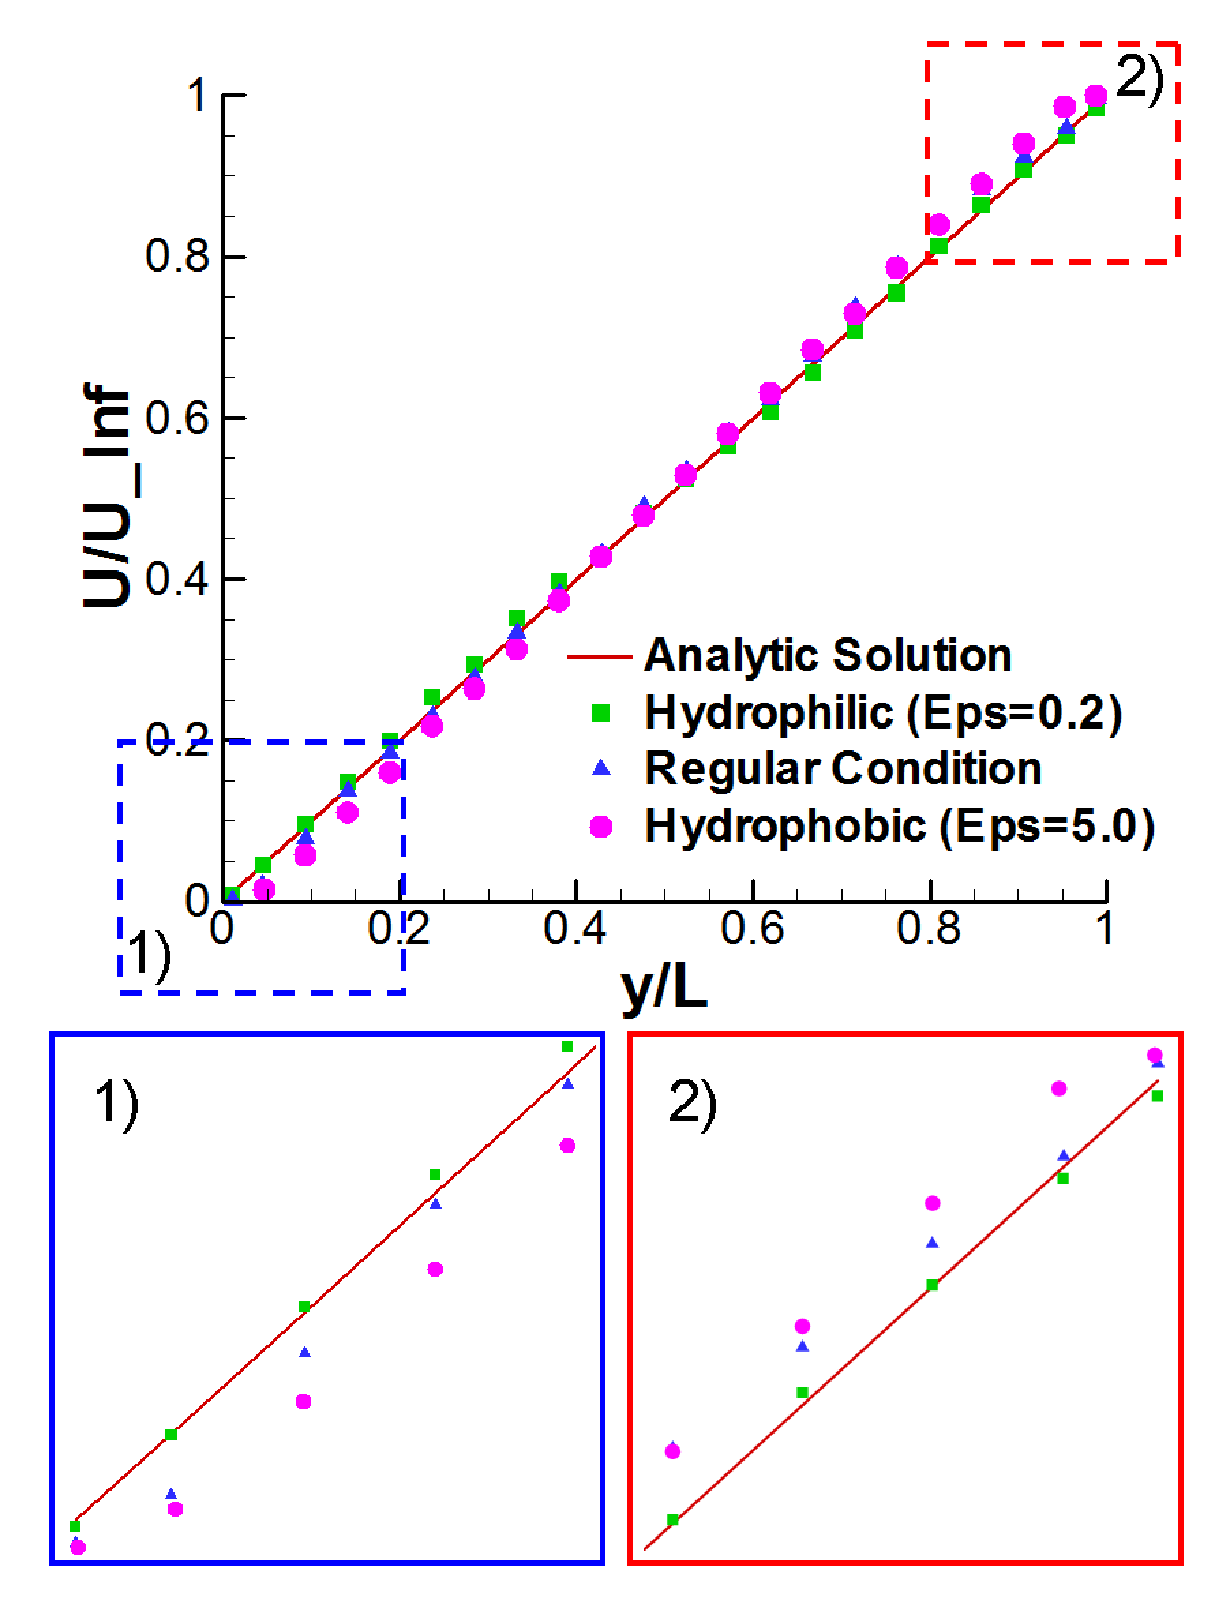
\includegraphics[width=0.9\linewidth]{MD_Solution_New.pdf}
%\vskip-0.2cm
%\caption{\small Steady Couette Flow Solution by Pure Molecular Dynamic Simulation; In normal condition (with the unique potential well depth between flow particle and surface material, denoted by $\epsilon$), the solution by MD is identical to the result of continuum approach. In hydrophobic case (smaller $\epsilon$) the fluid shows a slight slip on the wall, while the fluid particle strongly attempts to stick to the wall in hydrophilic case (bigger $\epsilon$).}
%\label{MD_Solution_New}
%\end{figure}


%The cost of force calculation to evaluate the potential energy is the slowest part of MD simulation. The computational cost of a classical MD simulation is very expensive, $\it O(N^{2})$ in $\it big O$ notation with $\it N$ particles, i.e. it will be demanded more and more CPU cost when the number of particle increase in MD simulation~\cite{Allen}.

%The above benefit of hybrid CFD-MD approach over pure CFD or pure MD simulations attracted the interest of many CFD and MD researchers, which resulted in the fast progress of hybrid schemes in 15 years since the first work~\cite{Thompson} was in press, as to be addressed in Section 2. Nevertheless, it is still very hard for an individual scientist to apply this approach to his/her domain of interest. We assume that the difficulty of  determining the state-of-the-art coupling condition is one possible reason. Even with accurate numerical schemes for solving each domain and coupling hybrid interface, the solution is strongly affected by the specification of coupling parameters. Layer size of data exchange zone with its position, sampling duration and the interval are major factors which affect the accuracy of coupled solution, and these conditions vary by the fluid and solid elements, flow condition and geometric characteristics. So far, there is no globally acceptable scheme for setting these coupling conditions. Thus, a number of numerical trial and erro are required to empirically determine the coupling condition for specific problem.

%In addition to the numerical endeavour of determining coupling condition between CFD and MD domains, there also exist computational challenges of integrating multiple application domains into a single problem set. Considering very different computational kernels (one could be mesh-based, the other unstructured particle simulations), it is nearly impossible to incorporate distinct CFD and MD codes under the umbrella of a single tightly-coupled application (i.e., binding two application codes within a single MPI communicator).

%One possible alternative will be to implement coupling interface on individual code and control these logically separated codes as a virtually unified simulation package. However, confined to parallel execution on conventional production system with batch queue, it cannot be guaranteed that two separate jobs will execute concurrently. Considering the computational characteristics of current application, where CFD and MD codes conduct frequent information exchange via their file interfaces, the first job to run will inevitably experience the idle waiting for its counterpart without the explicit support for co-scheduling. Another important challenge is the need for efficient load-balancing which takes into account the individual application's performance. Even if the two simulations could run concurrently, without explicit load-management/balancing support, there is likely to be inefficient utilization of compute resources due to load imbalance. As the performance of each simulation component changes with computing resource and problem size, re-adjustment of allocated resources to each task according to their performance is required during the simulation.


%Collectively, we are focusing on investigating numerical issues of applying the hybrid CFD-MD scheme to a nano-fluidic system, as well as designing and developing an efficient runtime framework for a coupled multi-component simulation. We consider the implementation of a 'generic' hybrid interface which can be easily attached to various kinds of incompressible CFD codes and MD packages, and the building of a 'portable' framework which is acceptable for most computer architectures. Regarding numerical simulations, we value our idea to determine coupling parameters is reasonable and easy to follow. Also we argue that our numerical experiments cover broader range of system scales and flow physics, than other individual works, though each simulation may not be the first trial for specific problem. Especially for physically unsteady flow simulation, our design of temporal coupling scheme can be one possible challenge to overcome the time-lagging in hybrid boundary.
%In view of computational science, we believe our trial is the first documented coupled multi-physics simulation utilizing a virtually unified simulation package, called ``Pilot-Job". We claim that there are several distinct advantages of using Pilot-Job: (i) obviates the need for a co-scheduler while preserving performance, (ii) enables dynamic resource allocation, which in turn is important for load-balancing across coupled simulations.

%We begin the next section with an outline of the concept and numerical issues of coupled simulations. Numerical details of individual code and implementation of hybrid scheme are presented in the next Section. Another objective of current research, the construction of an efficient CFD-MD simulation framework, will be discussed in Section 4. In Section 5, we will demonstrate our numerical results of a famous time-accurate validation problem (Couette flow simulation) and the physically unsteady flow simulation (oscillating boundary problem), as well as the performance of this coupled simulation, which will prove the accuracy and efficiency of our hybrid simulation framework. Finally, our next plan and the summary of current work are expressed in Section 6 and 7.

% ===== End of Former Version =====



% -------------------------------------------------------------------------
%\section{Development of A Hybrid CFD-MD Simulation Toolkit: Numerical Techniques for Multi-physics Flow Simulation}
\section{Fundamentals of the Hybrid Coupled CFD-MD Simulation Toolkit}
\label{sec:numerical}

The accuracy of a hybrid CFD-MD solution is governed by the underlying numerical schemes in individual solver as well as hybrid schemes implemented. We explain the features of baseline solvers and the structure of hybrid interface in this section. We also investigate additional numerical treatments to improve the accuracy of hybrid CFD-MD simulations in various types of fluid systems.
\Nkimnote{
\\=========== Modified version from ME ===========\\
The accuracy of a hybrid CFD-MD solution is governed by the underlying numerical schemes of the individual continuum and particle solvers as well as the coupling scheme. This section details and explains the features of baseline solvers and the structure of the hybrid coupling interface. Additional numerical treatments to improve the accuracy of hybrid CFD-MD simulations in various types of fluid systems are also addressed.
\\}

%\subsection{The Hybrid CFD-MD Approach}
\subsection{Overview of the Continuum-Molecular Coupled Approach}
The hybrid CFD-MD approach stands on the proposition that the molecular dynamic simulation produces more accurate solution than the continuum model and a more efficient continuum solver provides the boundary condition to particle domain without restricting the high degree-of-freedom of atomistic motion. So, the region which contains a strong flow gradient is resolved by a molecular dynamic simulation and moderate flow in macroscopic scale is captured by the continuum dynamics. Also, these problem domains overlap each other in the middle to exchange the individual information.

A detailed structure of the fluid domain for constrained Lagrangian dynamics models is described in Fig.~\ref{Fig:Couette}. CFD approach solves the external zones with the moderate flow velocity and MD analyzes the complex microscopic flow feature near the stationary obstacle or in the low-speed region. Hybrid region is placed sufficiently far from the solid obstacle to prevent the direct influence of strong fluctuation near the solid-fluid interface. Also, this region is designed sufficiently large to contain five layers with enough spacing.

Roles of these layers in hybrid region are as follows.
From the bottom, we have the {\it{particle-to-continuum}} and {\it{continuum-to-particle}} (denoted as 'MDtoCFD' and 'CFDtoMD', respectively) boundary zones for CFD and MD simulations, and have additional zone to exert external force. These three interesting zones are isolated by the buffer in between.
Particles' properties spatially located in the MDtoCFD boundary layer are averaged over a finite time (called 'sampling duration') and they are transferred to continuum solver at constant period (called 'sampling interval'). The height of each layer is the same as the CFD cell height and averaged conservative properties in two consecutive layers are passed to continuum domain to be directly imposed as the viscous boundary condition on the Navier-Stokes solver with collocated data structure.
Next, the hybrid MD boundary zone is placed in the middle. In this region, the instantaneous continuum solution is transferred to MD code. Particles in this layer are guided to eventually follow this macroscopic flow velocity, by solving a constrained Lagrangian dynamics equation. The strong point of this equation is that, molecules are led to follow the macroscopic flow property, while preserving their degree-of-freedom of translational motion.
In the uppermost layer, the external force is exerted on particles to conserve system's statistical ensembles. This force function is designed not too strong to influence the motion of particles in the domain of interest nor not too weak to have particles drifting away. %Preferably, the effective force needs to correspond to the mean pressure of the MD system~\cite{Werder}.
Finally, buffer layer is positioned in between each layer. This layer is set up to be bigger than the length scale of interacting particles (cutoff radius), not to have a solution in one layer being directly interfered by another solution.

\Nkimnote{
\\=========== Modified version from ME ===========\\
The hybrid CFD-MD approach stands on the proposition that (a) the molecular dynamic simulation produces a more physically accurate solution in its domain than the continuum model would, (b) a faster and more efficient CFD solver provides a physically accurate solution in the continuum domain, which would be prohibitive if a particle representation were to be used, and (c) the two solutions can be reconciled by the mutual exchange of information, the continuum solution providing the constraint to the particle solution while the latter providing a boundary condition to the former. So, the region within which molecular-level physics are important (e.g. a material interface) is treated and resolved by a molecular dynamic simulation, while the region within which the continuum-level physics adequately represent the transport processes on a macroscopic scale is treated and resolved by the continuum CFD. The continuum and particle (molecular) domains overlap, in this approach, so as to exchange information for the coupling. Obviously, the overlap domain must be one where both treatments/formulations are valid.
A detailed structure of the various domains associated with the hybrid CFD/MD methodology is described in Fig. 1. CFD solves the continuum equations in the �Pure CFD Region�, while MD resolves the microscopic (particle) flow in the �Pure MD region�. The latter is a solid stationary wall for the two test problems examined herein. The hybrid (overlap) region is placed sufficiently far from the solid wall to prevent direct constraint of the molecular-level physics in the proximity of the solid-fluid interface. 
This overlap region is designed sufficiently large to contain five individual layers of sufficient width for the purpose of their existence. The widths of these layers are of course problem dependent. Their roles in the hybrid region are as follows. One layer (the bottom one in Fig. 1-left) provides information from the particle (MD) domain to the continuum one (denoted as �MDtoCFD�). A second layer (the third one from the bottom in Fig. 1-left) provides information from the continuum domain to the particle one (denoted as �CFDtoMD�). A third layer (the top one in Fig. 1-left) applies a fictitious external force which prevents particles from escaping from the hybrid domain. These three �active� layers are separated by buffer layers, which are placed so as to ensure smooth transitions and that there is no direct correlation between the �active� layers. Properties (e.g. velocity) of particles spatially located in the MDtoCFD layer are ensemble-averaged over all the particles in the layer and also averaged over a finite time (�sampling duration�). The average value is communicated to the continuum solver periodically with a fixed period (�sampling interval�).
The height of each layer is the same as the CFD cell height and averaged conservative properties in two consecutive layers are passed to continuum domain to be directly imposed as the viscous boundary condition on the Navier-Stokes solver with collocated data structure. The CFDtoMD layer imposes the instantaneous values of properties, velocity in this case, resulting from the continuum solver. This is done via and appropriate constraint to the MD particle-based conservation of momentum on every single particle (constrained dynamics) in the CFDtoMD layer. Thus, particles in this layer are constrained to attain the macroscopic flow property (velocity in this case) on average, while preserving their degree-of-freedom of translational motion. In the uppermost layer, a fictitious external force is exerted on particles to prevent them from escaping the particle domain. This force function is designed to be short-range so as not to be strong enough to influence the motion of the particles past the buffer layer in the CFDtoMD domain. The force stiffens as the particles approach the location where the force becomes infinite in a way that minimizes reflections while preventing the particles from drifting out of the particle domain. The buffer layers existing in between each �active� layer are set up to be wider than the interaction length scale of the particles (cutoff radius), in order to prevent direct interaction between particles in neighboring �active� layers.
\\}

\skonote{It would be better to explain a little more detail on last sentence. Let's say the buffer between CFDtoMD and MDtoCFD boundary is smaller than cutoff length. Then, a solution at CFDtoMD (constrained MD) directly affects the motion of particles at MDtoCFD. And this is used for CFD boundary condition. This results that, CFD solution at CFDtoMD is the result of flow variation in MDtoCFD boundary, which in turn is directly affected by the CFDtoMD solution. Thus, solution at CFDtoMD becomes the boundary condition of CFD domain.}


%%%%% FIGURE %%%%%
\begin{figure}
\centering
%\vspace{-1em}
%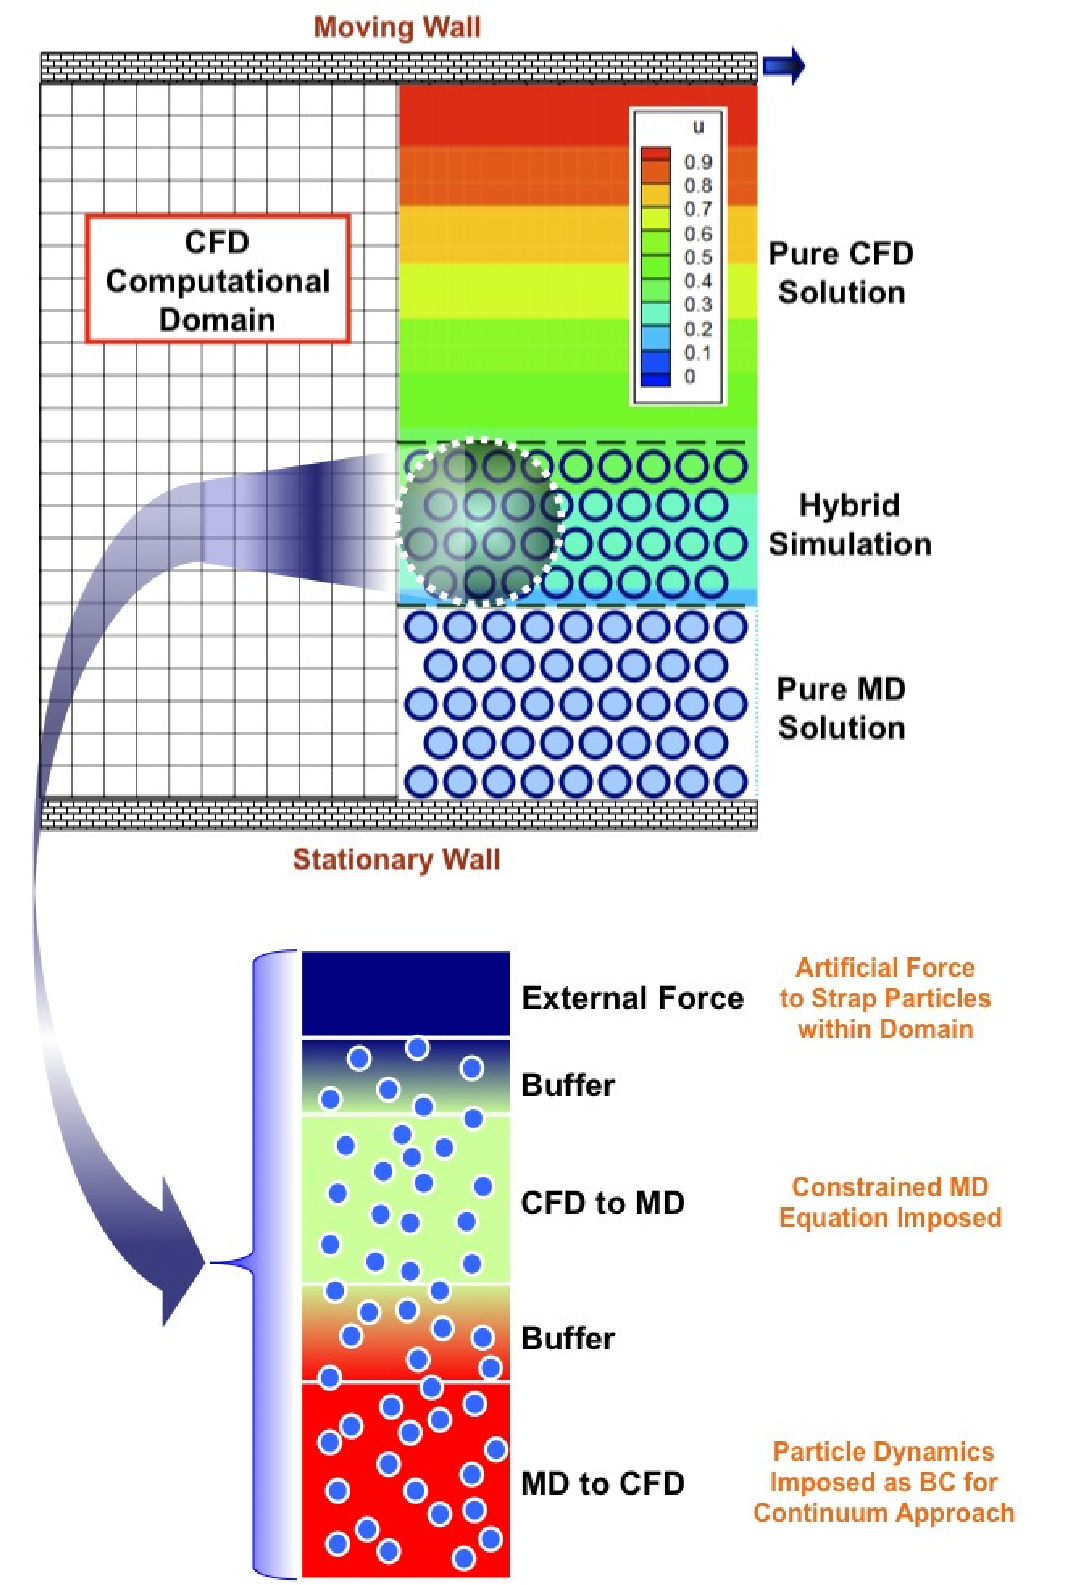
\includegraphics[scale=0.5]{fig1.pdf}
%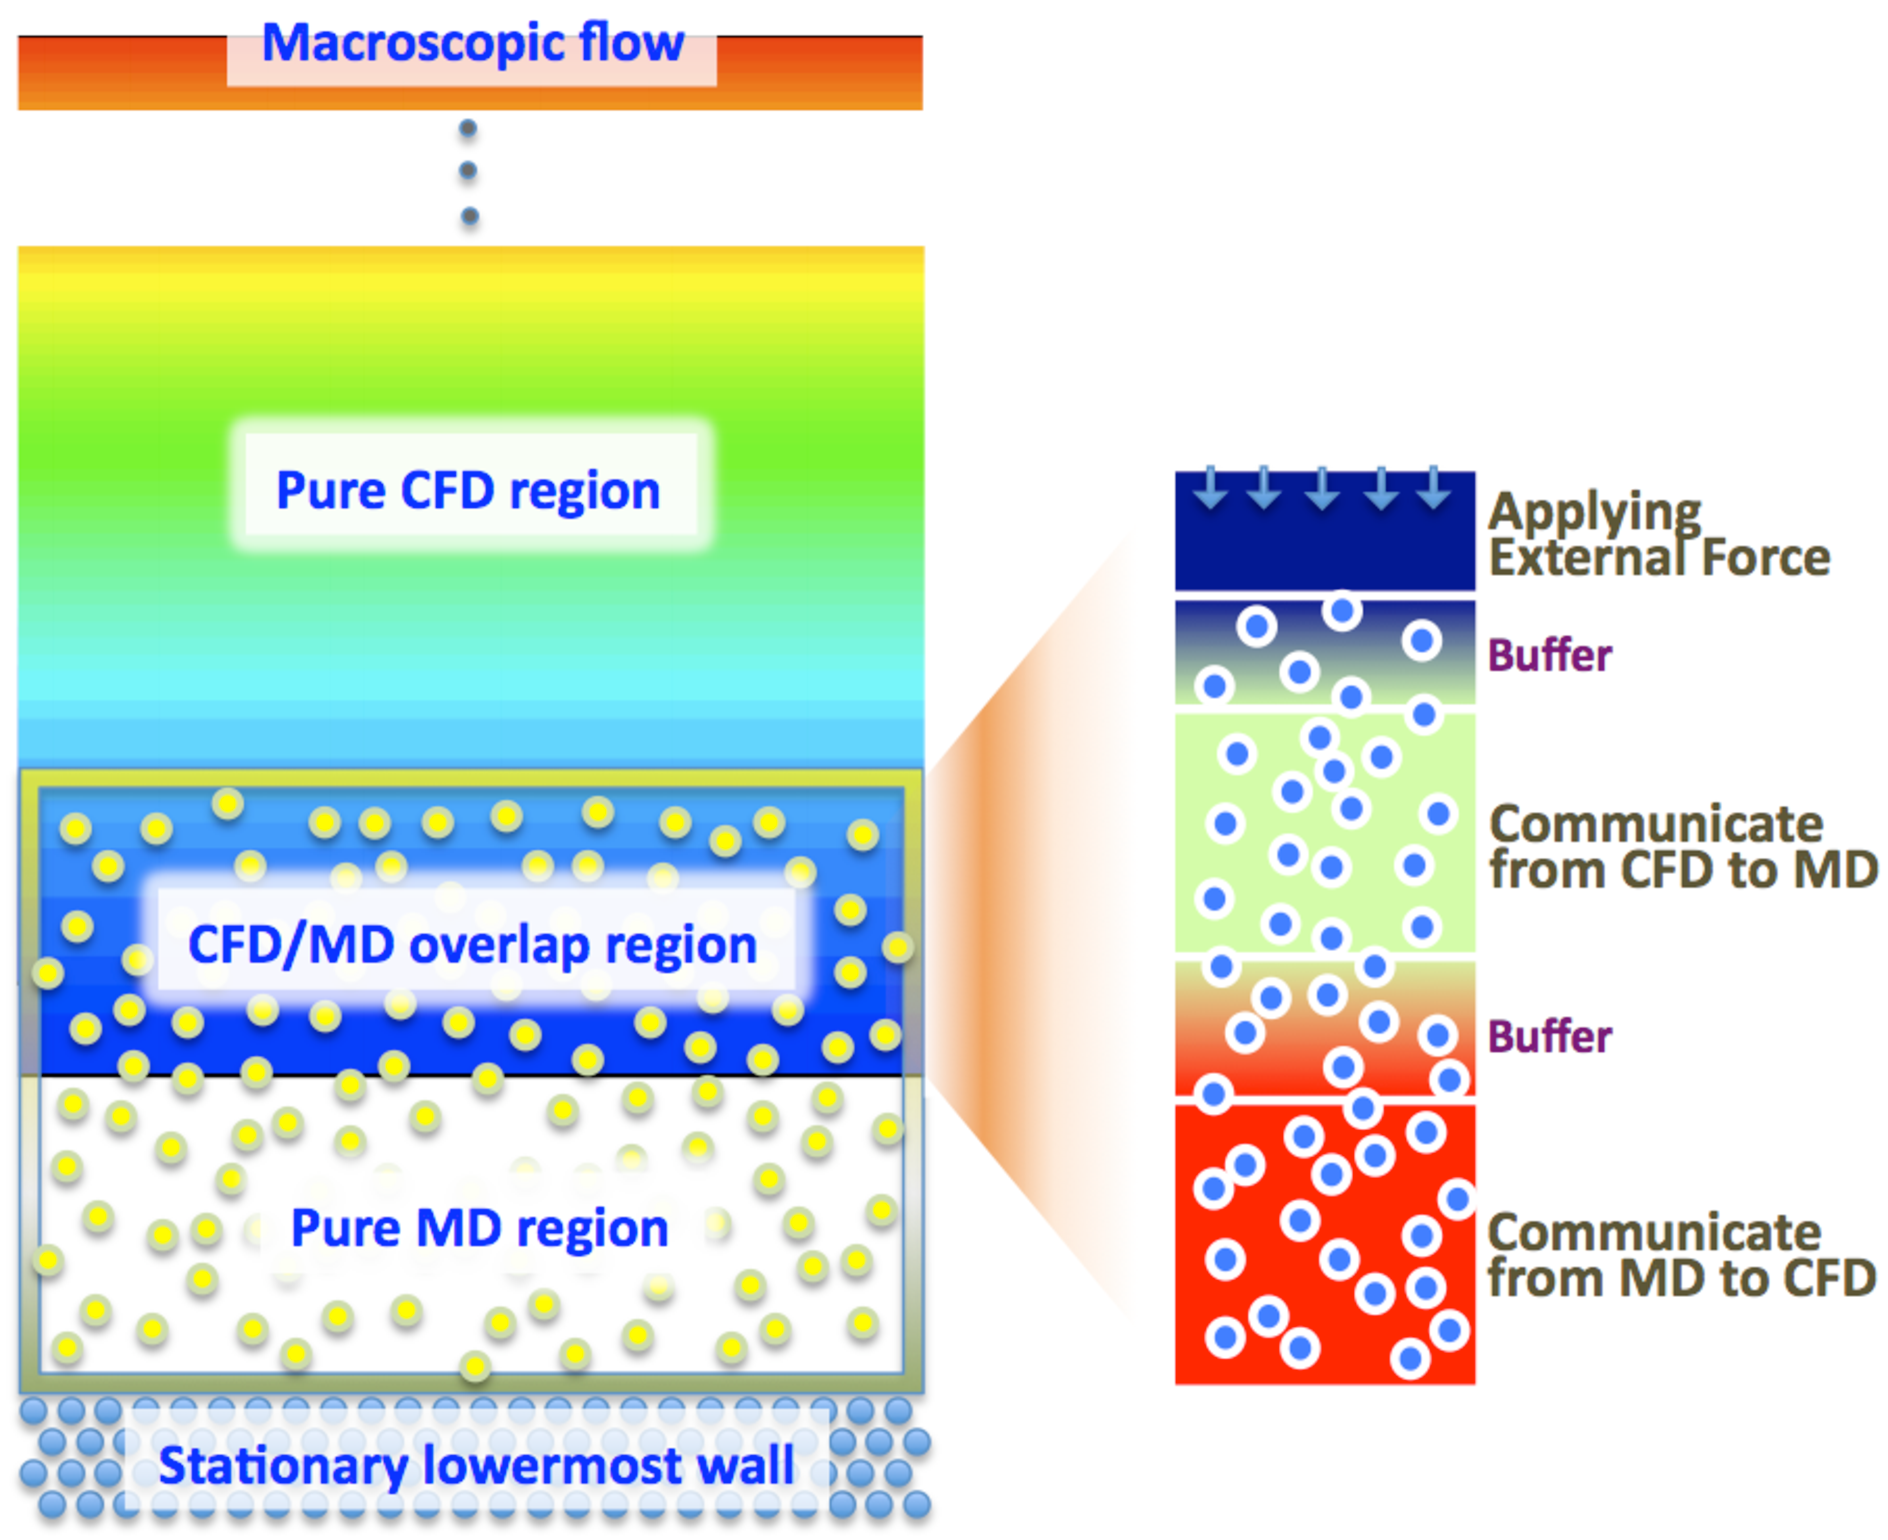
\includegraphics[scale=0.3]{Couette7.pdf}
%\linebreak
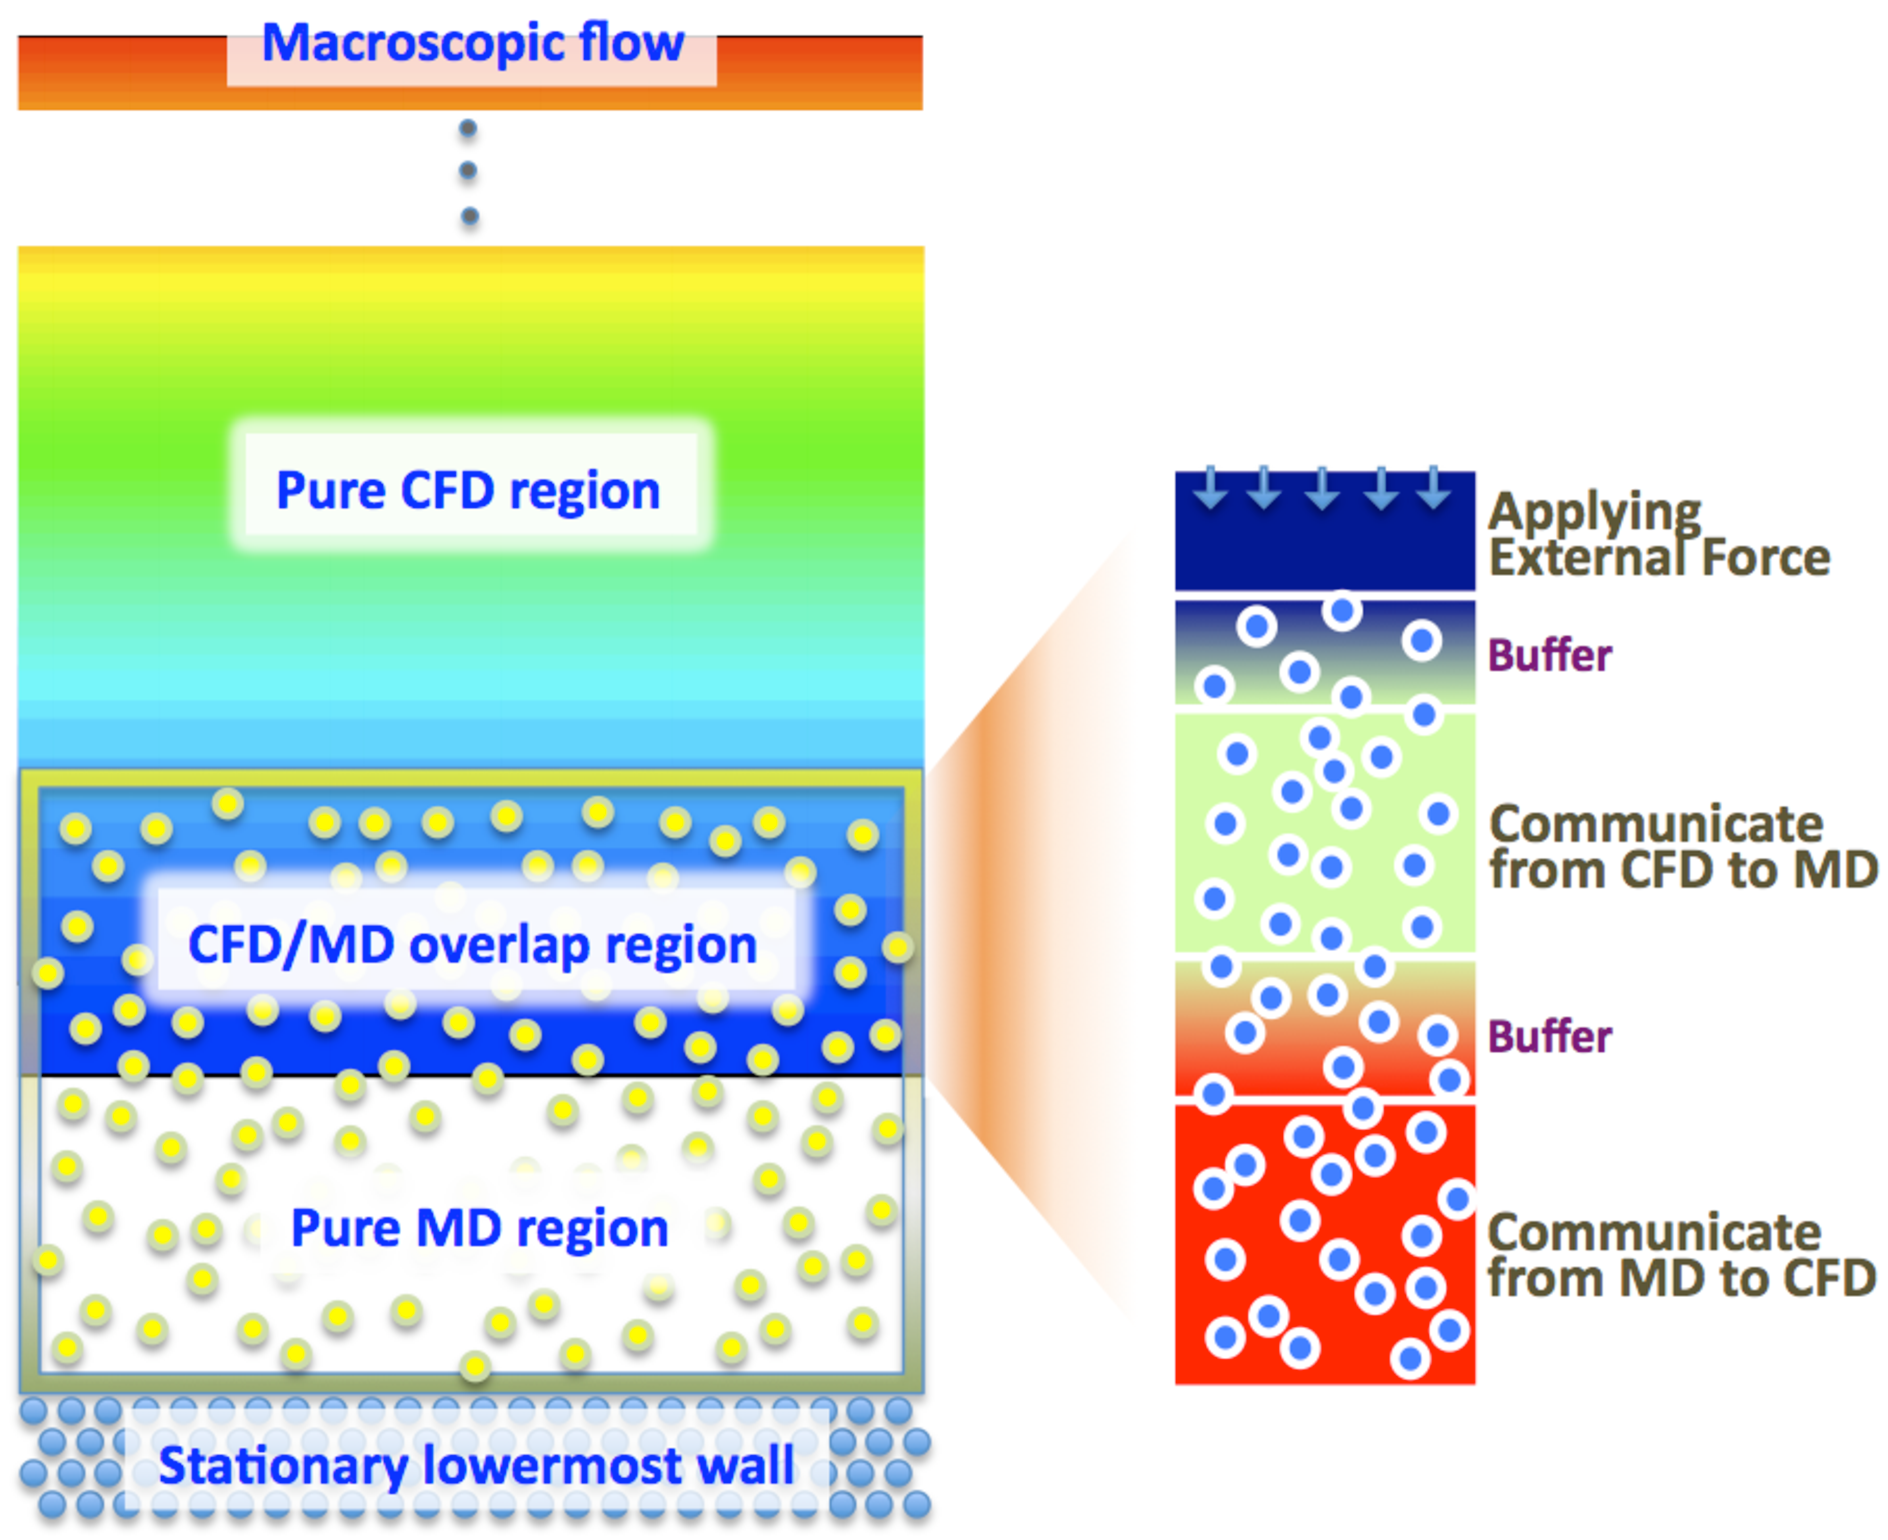
\includegraphics[width=0.8\linewidth]{Hybrid_Schematic.pdf}
%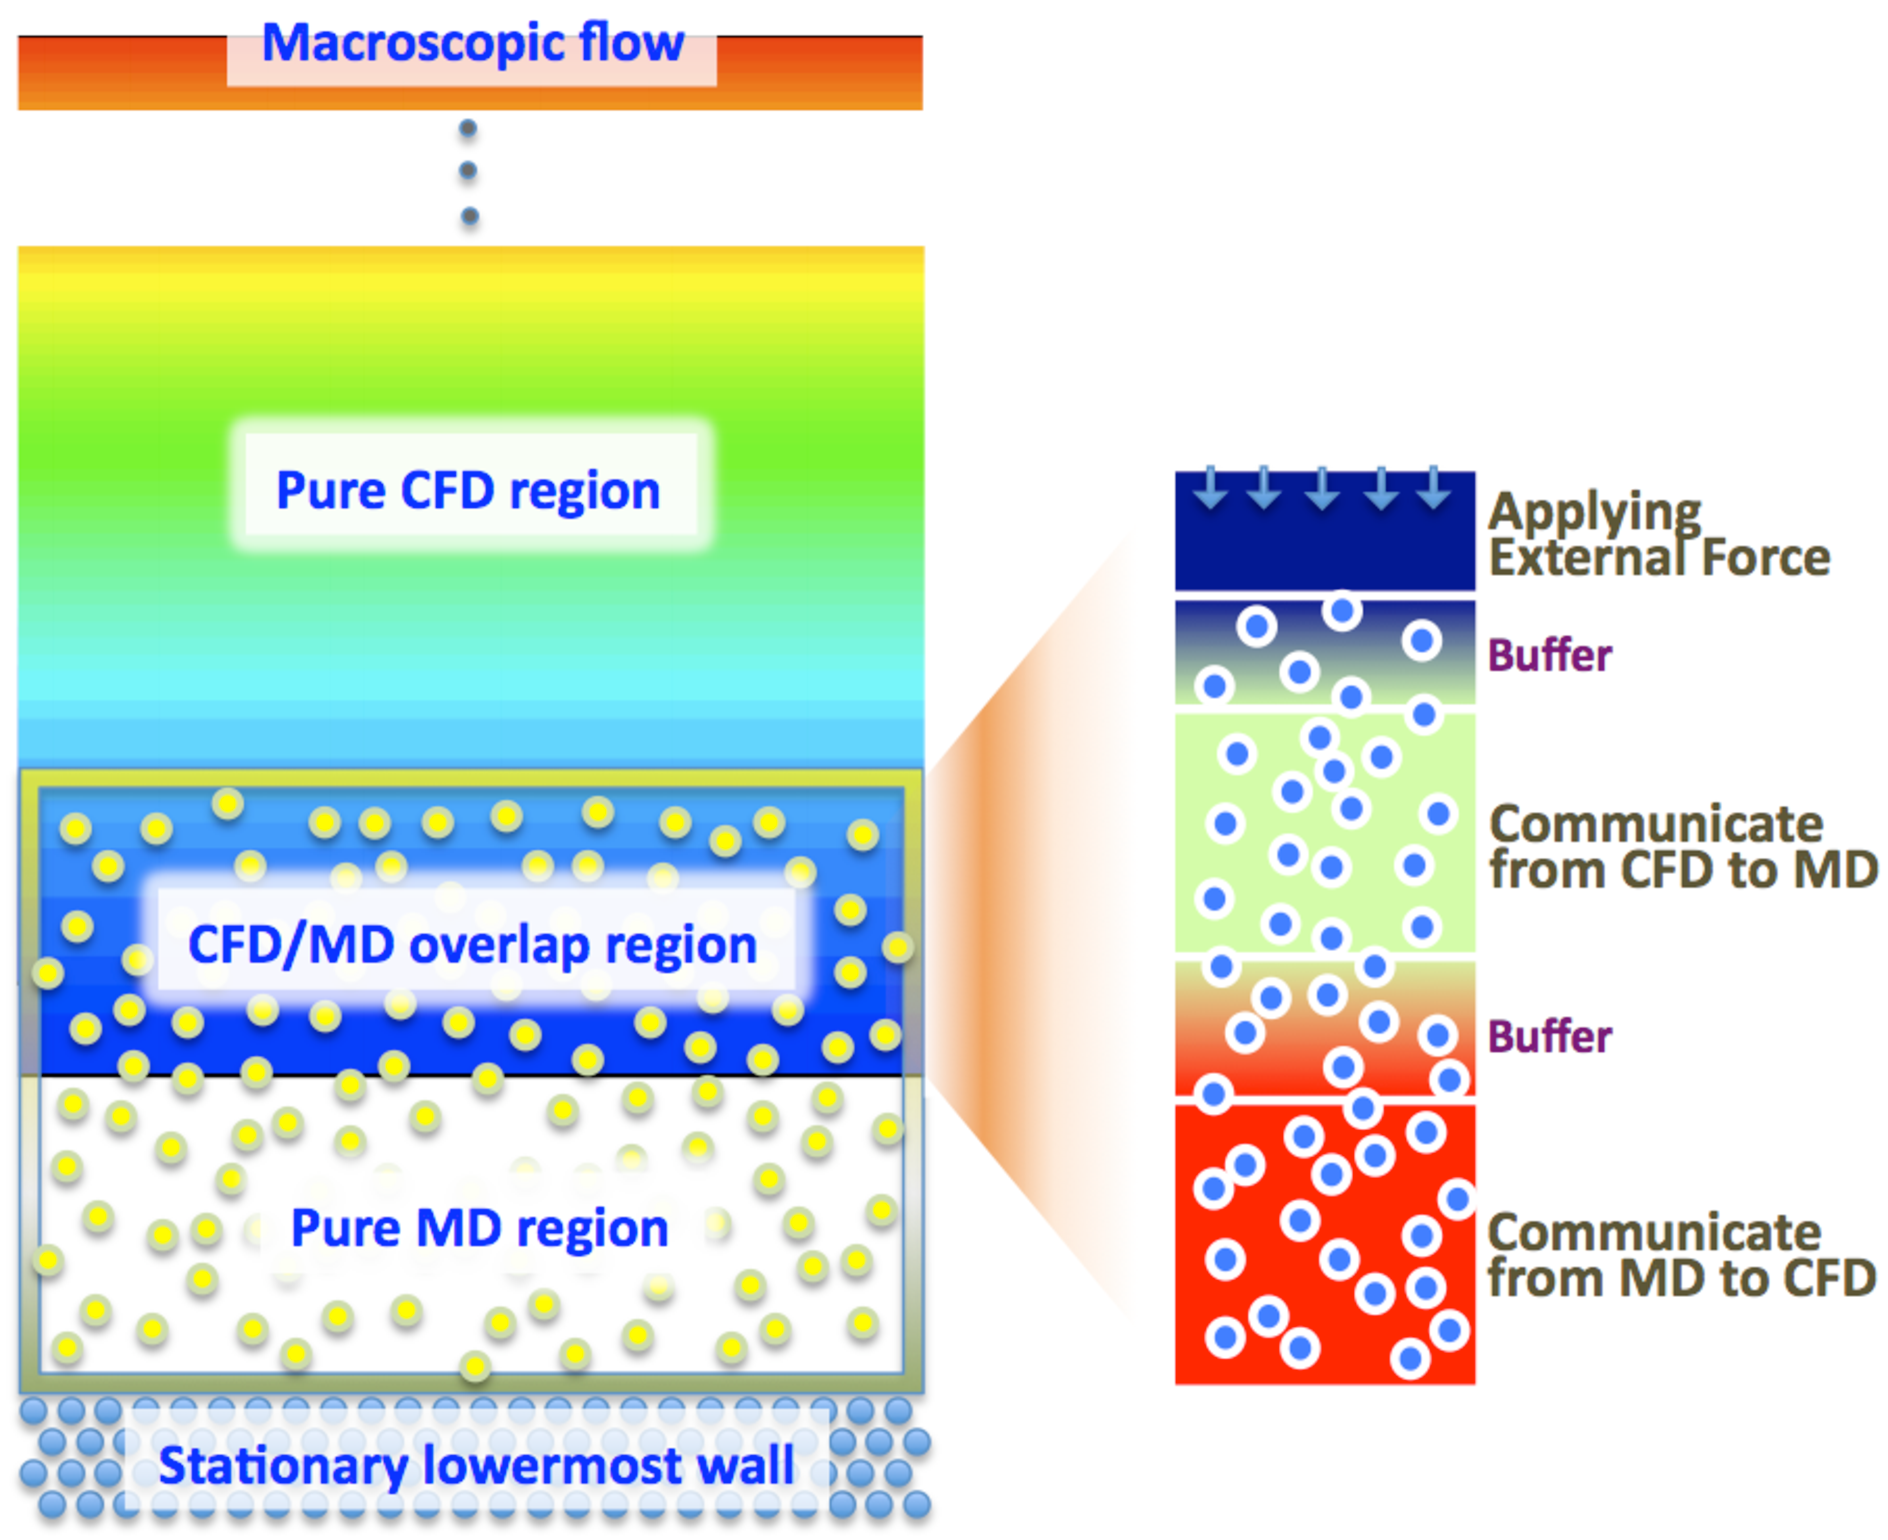
\includegraphics[width=1.0\linewidth]{Couette7.pdf}
\vskip-0.2cm
\caption{\small Schematic Diagram of the Hybrid Domain with Detailed View of Overlapping Zone; Overall continuum/atomistic computational domain including overlap region is shown on left figure. Detailed layer by layer explanation of overlapping region is indicated by right figure.
\Nkimnote{Modified version from ME :
Schematic diagram of the overall continuum/atomistic and hybrid computational domains for the chosen test problems (left) including a detailed view of the overlapping zone (right)}
}
\label{Fig:Couette}
\vspace{-1em}
\end{figure}
%%%%% FIGURE %%%%%



%\subsection{Numerical Schemes in the Baseline CFD and MD Codes}
\subsection{Governing Equations and Numerical Schemes}

\subsubsection{Continuum Incompressible Flow Formulation (CFD)}

The current in-house continuum hydrodynamics code solves the unsteady incompressible Navier-Stokes equations to demonstrate the isothermal nano-scale flow field:
\Nkimnote{
\\=========== Modified version from ME ===========\\
The current in-house continuum hydrodynamics code solves the unsteady incompressible Navier-Stokes equations: 
\\}

\vspace{-.2em}
%\vskip-.6cm
\begin{eqnarray}
\frac{\partial {u}_{i}}{\partial {x}_{i}} = 0
\end{eqnarray}
%\vspace{-.2em}
\vskip-.6cm
\begin{eqnarray}
\frac{\partial {u}_{i}}{\partial t} + \frac {\partial} {\partial {x}_{j}} ({u}_{i}{u}_{j}) = -\frac {\partial p} {\partial {x}_{i}} + \nu \frac {{\partial}^2 {u}_{i}} {{\partial} {x}_{j} \partial {x}_{j}} \nonumber
\end{eqnarray}
where $\nu$ is the kinematic viscosity.

%The primary difficulty in solving the incompressible Navier-Stokes equations in primitive variables stems from the lack of a time derivative in the continuity equation. There is no straightforward way to iteratively march these equations in time and ensure a divergence-free velocity field.

In this work, the pseudo-compressibility method~\cite{PseudoCompressibility} is adopted to form a hyperbolic system of equations which can be marched in pseudo-time.
%The method is extended to solve time-dependent problems by using sub-iterations in pseudo-time at each physical time step.
A time derivative of pressure is added to the continuity equation resulting in

%\vskip-.6cm
\vspace{-.2em}
\begin{eqnarray}
\frac{\partial (p/\rho)}{\partial \tau} = - \beta \frac{\partial {u}_{i}}{\partial {x}_{i}}
\end{eqnarray}
where $\beta$ denotes a pseudo-compressibility parameter, currently set up to 2.5.

For time-accurate unsteady simulation, a dual time stepping method is adopted and it is combined with the LU-SGS (Lower-Upper Symmetric Gauss-Seidel) scheme~\cite{LU-SGS} for the implicit time integration. The inviscid fluxes are upwind-differenced using Osher's flux-difference splitting scheme~\cite{Osher}. For higher-order spatial accuracy, the MUSCL (Monotone Upstream-centered Schemes for Conservation Laws)~\cite{MUSCL} approach is used on an inviscid flux calculation. Viscous fluxes are calculated using conventional second-order central differencing.


\subsubsection{Molecular-Level Formulation (MD)}

%Molecular dynamics computer simulation technique is a specified computer simulation method for molecular systems, including microscopic details of a system and macroscopic statistical properties, which are the properties of the atoms, the interactions between particles, molecular characteristics, structure of molecules, transport phenomena etc.~\cite{Allen},\cite{Haile},\cite{Rapaport}

%Concise MD part -- Start
%In MD, an initial velocity is assigned to each atom, and Newton's laws are employed at the atomic level to propagate the system's motion through time evolution:

%\vspace{-.2em}
%\begin{equation}
%F_{i} = m_{i}a_{i}
%\label{eq:Newton}
%\end{equation}
%\normalsize
%here each atom $\it i $ in a system constituted by N atoms, mi is the mass of i$^{th}$ atom, ai is the acceleration and denote by $\it {d^2r_{i}} / {dt^2}$, and $\it F_{i}$ is the force on i$^{th}$ atom, due to the atomic interaction which is calculated based on the potential energy between individual particles.

%The simplest choice for the potential energy $\it U(r)$  can be written as the sum of pairwise interactions of particles:

%\vspace{-.2em}
%\begin{equation}
%U(r_{1}, ...  ,r_{N}) =  \displaystyle\sum_{i} \displaystyle\sum_{j>i}  u(|r_{i} - r_{j}|)
%\label{eq:PEnergy}
%\end{equation}
%\normalsize
%where $\it i$ and $\it j$ particles are located at $r_{i}$ and $r_{j}$, and only $\it j>i$ cases have been considering for each particles pair once.

%The most commonly used two-body interaction model is the Lennard-Jones (12-6) potential is applied to calculate pairwise interaction and is define as:

%\vspace{-.2em}
%\begin{equation}
%u(|r_{i} - r_{j}|) = 4\epsilon_{ij}[(\frac{\sigma_{ij}}{r_{ij}})^{12}-(\frac{\sigma_{ij}}{r_{ij}})^{6}]
% \label{eq:LJ12}
%\end{equation}
%\normalsize
%where $\epsilon_{ij}$ and $\sigma_{ij}$ denote the pairwise potential well depth and the atom size parameter respectively, and $\it r_{ij}$ is the distance between the particle $\it i$ and $\it j$. The term $\it 1/r_{ij}^{12}$ dominating at short range distance repulsive behavior based on the Pauli principle to avoid overlapping the electronic clouds when particles are  brought very close to each other. The term $\it 1/r_{ij}^6$ dominates at long range attractive forces by van der Waals dispersion forces. The cut-off distance $\sigma_{c}$ is introduced here to reduce the computational cost and is set to be 2.2$\sigma$~\cite{Travis}.

%The time integration algorithm is required to integrate the equation of motion of the interacting particles and computing molecular trajectories, one of most common velocity Verlet algorithm is employed to compute the simulation.

%In this work,  the MD simulations were performed by using the modified version of Large Atomic Molecular Massively Parallel Simulator(LAMMPS). It is the classical molecular dynamics open-source code written in C++ and developed by Sandia National Labs.~\cite{LAMMPS}
%Concise MD part -- End

In MD, an initial velocity is assigned to each atom, and Newton's laws are employed at the atomic level to propagate the system's motion through time evolution. To calculate pairwise interactions of particles in the system,  the most commonly used Lennard-Jones (12-6) potential interaction model is employed and is define as:
\Nkimnote{
\\=========== Modified version from ME ===========\\
In MD, an initial velocity is assigned to each atom, and Newton�s conservation of momentum is employed at the atomic level to propagate the system�s motion through time evolution. In this work the most commonly used Lennard-Jones (12-6) intermolecular force potential model is employed to calculate pair-wise interactions of particles in the system, and is defined as: 
\\}
\vspace{-.2em}
%\footnotesize
\begin{equation}
 u(|r_{i} - r_{j}|) = 4\epsilon_{ij}[(\frac{\sigma_{ij}}{r_{ij}})^{12}-(\frac{\sigma_{ij}}{r_{ij}})^{6}]
 \label{eq:LJ12}
\end{equation}
\normalsize

where $\epsilon_{ij}$ and $\sigma_{ij}$ denote the pairwise potential well depth and the atom size parameter respectively, and $\it r_{ij}$ is the distance between the particle $\it i$ and $\it j$. The term $\it 1/r_{ij}^{12}$ dominating at short range distance repulsive behavior based on the Pauli principle to avoid overlapping the electronic clouds when particles are  brought very close to each other. The term $\it 1/r_{ij}^6$ dominates at long range attractive forces by van der Waals dispersion forces. The cut-off distance $\sigma_{c}$ is introduced here to reduce the computational cost and is set to be 2.2$\sigma$~\cite{Travis}.

The time integration algorithm is required to integrate the equation of motion of the interacting particles and computing molecular trajectories, one of most common velocity Verlet algorithm is employed to compute the simulation.

In this work,  the MD simulations were performed by using the modified version of Large Atomic Molecular Massively Parallel Simulator(LAMMPS). It is the classical molecular dynamics open-source code written in C++ and developed by Sandia National Labs.~\cite{LAMMPS}

\Nkimnote{
\\=========== Modified version from ME ===========\\
where  $\epsilon_{ij}$ and $\sigma_{ij}$ denote the pair-wise potential well depth and the atom size parameter respectively, and rij is the distance between the particle i and j . The repulsive term 1 /rij12 dominating at short rij distance is based on the Pauli principle to avoid overlapping the electronic clouds when particles are very close to each other. The attractive term 1/rij6 dominates at long range representing Van der Waals dispersion forces. A cut-off distance $\sigma_{c}$  is introduced here to reduce the computational cost and is set to be 2.2$\sigma$  [28]. Namely when rij exceeds the cutoff the intermolecular force is set to zero without being calculated.
The most common velocity Verlet algorithm is employed for time integration of the equations of motion of the interacting particles and to compute molecular trajectories in the simulation. 
In this work, the MD simulations were performed by using an appropriately modified version of the Large Atomic Molecular Massively Parallel Simulator (LAMMPS). It is a classical molecular dynamics open-source code written in C++ and developed by Sandia National Labs. [29]
\\}


%\subsection{Implementation of Hybrid Interface}
\subsection{Hybrid Interfaces and Schemes}
The hybrid simulation requires the implementation of hybrid interfaces and schemes on individual code. In the current study, the file interface is designed to schedule the information exchange between continuum and discrete particle descriptions.  A constrained Lagrangian dynamics model is implemented for hybrid simulation. Unit conversion routine is also implemented in the application code. These changes are summarized in table~\ref{table:interface_implementation}.


% Table formats; h,t,b,p - here,top,bottom,page of floats
%\begin{table}[t]
\begin{table}
  \caption{\small Implementation of Hybrid Interface on CFD and MD Codes. Both codes are equipped with the file-based information exchange routine, to update the hybrid boundary condition. CFD code experiences the global change of its data structure to store the information of the entire fluid system. MD code adopts hybrid equations to impose the macroscopic information on microscopic domain and to ensure numerical stability.}
  \label{table:interface_implementation}
  \centering
%  \resizebox{0.8\linewidth}{!} {
\footnotesize
 \begin{tabular}{>{\centering}p{0.15\linewidth} || p{0.3\linewidth} | p{0.3\linewidth} }
\hline
  & \centering CFD & \multicolumn{1}{c}{MD} \\
\hline
 Global Change & Overset Data Structure (\it{optional}) & \multicolumn{1}{c}{-} \\
\hline
 \centering External Force & \centering - & External Force Equation (Eqn.~\ref{eq:External_Force}) \\
\hline
% CFDtoMD &  - File Interface: Sender & {- File Interface: Receiver \\ - Constrained MD Equation (Eqn.~\ref{eq:Con3})} \\
 \multirow{2}{*}{CFDtoMD} &  \multirow{2}{*}{File Interface: Sender} & {File Interface: Receiver} \\
 & & Constrained MD Equation (Eqn.~\ref{eq:Con3}) \\
\hline
 MDtoCFD & File Interface: Receiver & File Interface: Sender \\
\hline
\end{tabular} %}
\vspace{-1em}
\end{table}


The CFD code employs the data structure of overset mesh technique~\cite{Chimera} to ease the handling of coupling parameters. In other words, the entire fluid domain is generated as the CFD mesh system and pure MD region is turned off as the `Hole' cell in the terminology of overset technique. Likewise, MDtoCFD and CFDtoMD boundary cells are declared as `Fringe' and `Donor' cells, respectively. The labor of mesh regeneration according to the change of coupling parameters (position and depth of hybrid layers) disappears with the overset data structure.

Both codes are equipped with the information exchange routine which consists of one file sender and one file receiver. These file interfaces are scheduled to turn on every sampling interval. The instantaneous properties in the Donor cells of continuum domain are transferred to MD site and referenced when applying constrained Lagrangian dynamics equation. Averaged molecular properties are sent to CFD domain and they are used as the boundary conditions of Fringe cells. All exchanged properties are written in MD unit: thus, CFD code is equipped with velocity unit conversion function and equation of state which changes the pressure solution from CFD site to equivalent density property in MD domain.

Along with the file interface, additional equations of motion are employed on MD code to accurately describe the influence of macroscopic flow variation on particle domain. First, the external force should be imposed to prevent leaving particles from the control domain and the force is applied to the normal direction of uppermost MD layer. A cost-effective classical external force model by Nie {\it{et al.}}~\cite{Nie} is employed as,

%\skonote{Or, shall we replace the last sentence to the follow? \\
%The design of external force is very important to exert the correct mean pressure on MD domain without local disturbance in the density field, as is expressed by Werder {\it{et al.}}~\cite{Werder}. Compared to other hybrid models, the external force design in constrained Lagrangian dynamics approach is less sensitive to the solution since particles in the buffer layer between external force layer and molecular dynamic boundary layer act as decreasing the influence of non-uniform density distribution. Thus, a cost-effective classical external force model by Nie {\it{et al.}}~\cite{Nie} looks still valid for acquiring the accurate solution.}

\vspace{-.2em}
%\footnotesize
\begin{equation}
 F_{ext, i} = -p_{a}\sigma\frac{y_{i}-Y_{n-1}}{1-(y_{i}-Y_{n-1})/(Y_{n}-Y_{n-1})}
 \label{eq:External_Force}
\end{equation}
\normalsize
where $\it p_{a}$ denote the average pressure in the MD region, $\it Y_{n}-Y_{n-1}$ is the thickness of the uppermost layer which is applied the force and $\it F_{ext}$ is the external force acting on $\it i^{th}$ particle located on position $\it y_{i}$.


Next, on CFDtoMD layer, the macroscopic flow properties at specific time shall be introduced to lead the motion of multiple particles in that layer. To satisfy mass conservation, a certain number of particles are inserted into or removed from this layer according to the mass flux by CFD solution,

\vspace{-.2em}
%\footnotesize
\begin{equation}
n = -A \rho u_y \Delta t / m
 \label{eq:Mass_Flux}
\end{equation}
\normalsize
where $A$ is the horizontal area, $u_y$ is the vertical velocity component by CFD solution and $\Delta t$ is the sampling interval.

A very complicated numerical intervention is required to maintain momentum conservation. The average velocities of particles in $\it J_{th}$ cell is equal to the velocity $\it u_{J}$ in continuum cell.

\vspace{-.2em}
%\footnotesize
\begin{equation}
 u_{J}(t) = \frac{1}{N_{J}} \displaystyle\sum_{i} v_{i}
 \label{eq:Con_vel}
\end{equation}
\normalsize
where $\it v_{i}$ is velocity of $\it i^{th}$ particle and $\it N_{J}$ is the number of particles in the cell. With taking Lagrangian derivative of Eq.~\ref{eq:Con_vel},

\vspace{-.2em}
%\footnotesize
\begin{equation}
 \frac{Du_{J}(t)}{Dt} =  \displaystyle\sum_{i} \frac{\ddot{x_{i}}}{N_{J}}
 \label{eq:Lagrangian}
\end{equation}
\normalsize

The Classical MD equation of motion can be generalized to obtain constraint by adopting the fluctuation in acceleration of each particles, $\zeta_{i}$

\vspace{-.2em}
%\footnotesize
\begin{equation}
 \frac{F_{i}}{m_{i}} = \ddot{x_{i}}(t)  =   \frac{Du_{J}(t)}{Dt} + \zeta_{i} = \frac{\displaystyle\sum_{i}F_{i}(t)} {\displaystyle\sum_{i}m_{i}} +   \zeta_{i}
 \label{eq:Con2}
\end{equation}
\normalsize
where $\it F_{i}$ is the force on $\it i^{th}$ particle based on the interactions between particles,  $\it m_{i}$ is mass of each atom and  Eqn.~\ref{eq:Con2} satisfies,
\vspace{-.2em}
%\footnotesize
\begin{equation}
\displaystyle\sum_{i}\zeta_{i}m_{i} = 0
 \label{eq:Con2}
\end{equation}
\normalsize

Finally, the constrained particle dynamics with conventional equation of motion can be written as:

\vspace{-.2em}
%\footnotesize
\begin{equation}
 \ddot{x_{i}}(t) = \frac{F_{i}}{m_{i}} -  \frac{\displaystyle\sum_{i}F_{i}(t)} {\displaystyle\sum_{i}m_{i}} - \frac{1}{\Delta t_{MD}} \{  \frac{\displaystyle\sum_{i}m_{i}\dot{x_{i}}} {\displaystyle\sum_{i}m_{i}} - u_{J}(t + \Delta t_{MD})\}
 \label{eq:Con3}
\end{equation}
\normalsize

The continuum velocity and the mean microscopic velocity from MD over control domain provide the synchronization of the mass and momentum consistent with Eqn.~\ref{eq:Con3}.


\subsection{Statistical Error and Coupling Parameters}
\label{sec:numerical_noise}

%Molecular dynamics inherently describes the fluctuating pattern of particles, which becomes a noise in CFD solution. How to reduce this statistical error~\cite{Hadjicon3,Time_Mechanism} of averaged MD profile determines the accuracy of CFD solution.

How to reduce the statistical error of averaged MD profile, which is the response of innate spatial/temporal locality in molecular dynamic systems, determines the accuracy of CFD solution in hybrid simulation. According to the mathematical expression in statistical error~\cite{Hadjicon3,Time_Mechanism}, the ratio of sampling noise compared to the macroscopic velocity is inversely proportional to the square root of spatial layer size and temporal sampling duration. For example, reducing the macroscopic velocity by half requires either 4 times larger system domain or 4 times longer sampling to maintain the same order of accuracy.
%\vspace{-.2em}
%\begin{eqnarray}
%E \propto \frac{1}{\sqrt{M}} \times \frac{1}{\sqrt{N}} \times \frac{1}{u_{\infty}}
 %\label{eq:noise}
%\end{eqnarray}
%where M is the number of independent samples, N is the number of particles spatially contained in that layer, and ${u_{\infty}}$ denotes the far field velocity.

% Eqn.~\ref{eq:noise} implies that the increase of system size or sampling duration is inevitable to solve the slower velocity field. Sampling duration is determined to be less than the sampling interval, which is chosen to be far smaller than the hydrodynamic characteristic time for time-accurate simulations. Since the hydrodynamic time scale is a function of characteristic size and kinematic viscosity, the sampling interval shall be fixed in solving the slower flow field. This, in turn, results in the impossibility to handle the sampling duration. Therefore, increasing the system size is the only possible way to maintain the same statistical accuracy, to be proportional to the square of the velocity change.


Sampling duration with interval, the size of sampling layer and its position are coupling parameters which define the scale and pattern of this noise. The layer size and sampling duration collectively work for reducing the noise, by increasing the spatial and temporal sampling scales. Sampling interval is a factor which restricts the sampling duration. On unsteady simulations, a short sampling interval is preferred to frequently update temporal variation of flow field in hybrid boundary zones. This interval acts as the upper bound of sampling duration. The location of the sampling layer is a secondary factor which can locally increase the strength of fluctuation. Conventionally, sampling layer is placed far from the solid obstacle, e.g., at least 10 $\sigma$ above the bottom wall in solving the flow of the liquid argon~\cite{Yen}.

We introduce two numerical ideas to acquire the accurate hybrid solution. One is to quantitatively measure the scale of statistical noise in particular domain and the other is to numerically get the acceptable solution. The former shows the initial guideline to determine the coupling parameter and the latter refines the accuracy of the former solution.


\subsubsection{Determining Coupling Conditions}
\label{sec:numerical_parameters}
The statistical noise is a function of the characteristics of fluid and surrounding solid elements, and geometric configurations, as well as the flow condition.
Unfortunately, previous analyses on the strength of statistical error~\cite{Hadjicon3,Time_Mechanism} fails to consider the stronger interaction near the fluid-solid interface and the shape of the domain. We sense that the clear coupling parameters can be determined after the look-up of that specific system


Our intuitive idea of numerically detecting the strength of statistical noise is to solve the stationary flow of the same fluid domain by pure MD method. The procedure is as follows.
\begin{enumerate}
\item Empirical design of the sampling interval and the sampling layer's position\footnotemark
\item Structure construction\footnotemark
\item Simulation and collecting the temporal history of sampled velocity\footnotemark
\item Data processing\footnotemark
\item Determining the sampling layer size and the sampling duration\footnotemark$^{,}$\footnotemark
\end{enumerate}


\footnotetext[1]{Sampling interval is designed less than $1/100^{th}$ of hydrodynamic characteristic time; The location of sampling layer is placed O(10) nanometers above the solid obstacle.}

\footnotetext[2]{The height of the domain can be reduced by placing a specular wall on the top, in case the system is sufficiently large; The length of the domain along the periodic direction can be arbitrarily chosen. The optimal length is further determined by the relation between the strength of noise and number of particles, i.e., $V_{noise}{\propto}1/\sqrt{N}$.}

\footnotetext[3]{Data collection starts as soon as the relaxation process is finished. Temporal history of averaged velocity from the smallest layer size with shortest sampling interval is stored.}

\footnotetext[4]{Produced dataset around the location of sampling layer is spatially and temporally averaged to produce the spatial and temporal variation of the sampled velocity.}

\footnotetext[5]{The noise is compared with the expected macroscopic velocity at that position, considering the linear velocity gradient from the wall to the far field. A paired condition which produces sufficiently small portion of noise and whose temporal duration is less than designed sampling interval is chosen to be the layer size and sampling duration of this hybrid simulation.}

\footnotetext[6]{If no condition is satisfactory, the acceptable condition can be obtained by either increasing the length of computational domain based on $V_{noise}{\propto}1/\sqrt{N}$ or changing the position of sampling layer and repeating data processing. The one condition which generates the smallest MD domain in the hybrid simulation is chosen.}

%Change the position of sampling layer and conduct data processing again in case no condition is satisfactory. Or increase the length of computational domain to reduce the noise by $V_{noise}{\propto}1/\sqrt{N}$. There exists infinite number of coupling conditions which produce the same amount of statistical noise: the one which requires the smallest MD domain for hybrid simulation is chosen.

We argue that our idea is very easy to follow and computationally not expensive since the solution of the stationary flow is immediately collected.
%The sampling noise in the specific system is quantified by this stationary flow simulation.
This stationary flow simulation provides the amount of sampling noise in various sampling conditions.
%Meanwhile, this experiment does not provide the statistical error because predicting the macroscopic velocity is impossible except restricted number of flow systems whose analytic solutions are present.
Meanwhile, this experiment does not provide the statistical error because of the impossibility to predict the macroscopic velocity expect some well-known flow systems. This necessitates us to investigate additional approach which is globally applicable.


\subsubsection{Sampling Multiple Independent Experiments}
\label{sec:numerical_lowspeed}
So far, all hybrid CFD-MD applications have been restricted to extremely fast flow field of O(100) m/s velocity.
The difficulty of solving moderate-speed flow field by a hybrid approach is explained as follows. The hydrodynamic time scale is expressed as a function of characteristic size and kinematic viscosity. This implies that the sampling interval is fixed regardless of the change in velocity. This, in turn, results in the impossibility to handle the sampling duration. Increasing the system size proportional to the square of the velocity change remains the only possible way to maintain the same statistical accuracy. Unfortunately, submitting excessively large-scaled simulation on public supercomputers unfavorably takes far long time to get allocated. In worse case, the simulation may exceed the capacity of the system. Thus, a different approach is necessary for efficiently simulating the low-speed flow field.

%Considering that the increase of the MD domain is technically bound by the computing capacity, a different approach is necessary for simulating the low-speed flow field.

We propose sampling multiple independent hybrid simulations from a smaller domain instead of trying to run a single hybrid simulation in the large domain.
%For this purpose, we design a framework which samples multiple independent hybrid simulations.
The initial velocity component at individual problem set is differently determined from a Maxwell-Boltzmann distribution and solutions from independent simulations are averaged to produce the final solution. The labour of manually administrating multiple job executions are resolved by using a BigJob framework, which is to be discussed in the Section~\ref{sec:computational}.

Along with the advantage in computing capability, sampling multiple experiments provides another advantage of less-sensitivity to coupling conditions. Even if the coupling parameters are ill-chosen, highly noisy individual solution can be refined by the enough number of independent samples. This advantage also increases the value of capturing the magnitude of statistical noise in Section~\ref{sec:numerical_parameters}, because the requirement of predicting the macroscopic velocity in the sampled layer becomes less important.
%Clear advantages of sampling multiple experiments are that the simulation is not bound by \textit{(1) computing capacity} and \textit{(2) flow characteristics} anymore.


\subsection{Temporal Coupling Schemes}
\label{sec:numerical_temporal}


%Two conventionally used coupling approaches of synchronized and sequential coupling strategies are depicted in Fig.~\ref{Hybrid_Timescale1}. In synchronized coupling, CFD and MD codes exchange the information in the overlapping region at each sampling interval (denoted by ${\Delta}t$) and independently evolve to the next exchange timestep. In contrast, one domain advances to the next exchange timestep and leads its counterpart to approach this point in sequential coupling. Comparing these two mechanisms, synchronized coupling clearly have a far better parallel efficiency compared to sequential coupling.~\cite{Time_Mechanism} Parallel performance in synchronized coupling can ideally reach the single code running in case an appropriate load-balancing between two domains is applied. Large overhead on waiting is inevitable in sequential way unless CFD and MD application components run in a single MPI communicator, which implies that two codes are unified. On the other hand, sequential approach is expected to produce more time-accurate solution because the boundary condition on following domain (CFD domain in the figure) is implicitly imposed.
%Time-lagging phenomenon in CFD boundary region is observed in both strategies, because averaged molecular dynamic properties over backward sampling duration (from $n{\Delta}t-{\Delta}t_{s}$ to $n{\Delta}t$) are used to impose the CFD boundary condition at that instance ($n{\Delta}t$). Thus, the extrapolation from previous MD solutions is necessary to eliminate the time-lagging by half of sampling duration (${\Delta}t_{S}/{2}$) in the CFD boundary zone.
Two conventionally used coupling approaches of synchronized and sequential coupling strategies are depicted in Fig.~\ref{Hybrid_Timescale1}. In synchronized coupling, CFD and MD codes exchange the information in the overlapping region at each sampling interval (denoted by ${\Delta}t$) and independently evolve to the next exchange timestep. In contrast, one domain advances to the next exchange timestep and leads its counterpart to approach this point in sequential coupling. Comparing these two mechanisms, synchronized coupling has a far better parallel efficiency because both codes independently evolve to the next sampling interval, while sequential approach is expected to produce more time-accurate solution because the boundary condition on following domain (CFD domain in the figure) is implicitly imposed. Unfortunately, both strategies contain the time-lagging phenomenon in CFD boundary region, because averaged molecular dynamic properties over backward sampling duration (from $n{\Delta}t-{\Delta}t_{s}$ to $n{\Delta}t$) represents the CFD boundary condition at that instance ($n{\Delta}t$). Extrapolation from previous MD solutions is necessary to eliminate the time-lagging by half of sampling duration (${\Delta}t_{S}/{2}$) in the CFD boundary zone.

%\begin{figure}[htbp]
\begin{figure}
\centering
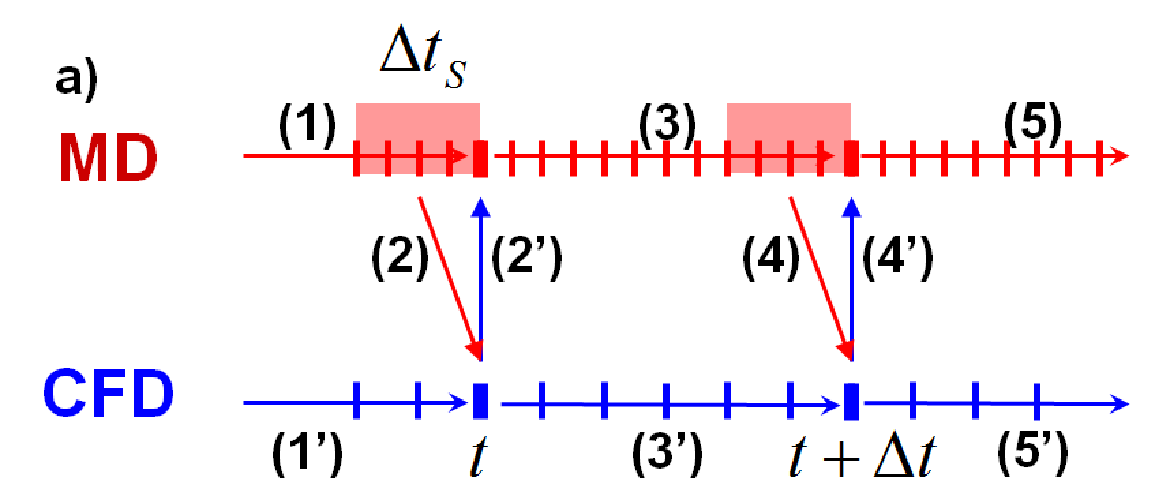
\includegraphics[width=0.8\linewidth]{Synchro_Coupling.pdf}
%\vskip-0.2cm
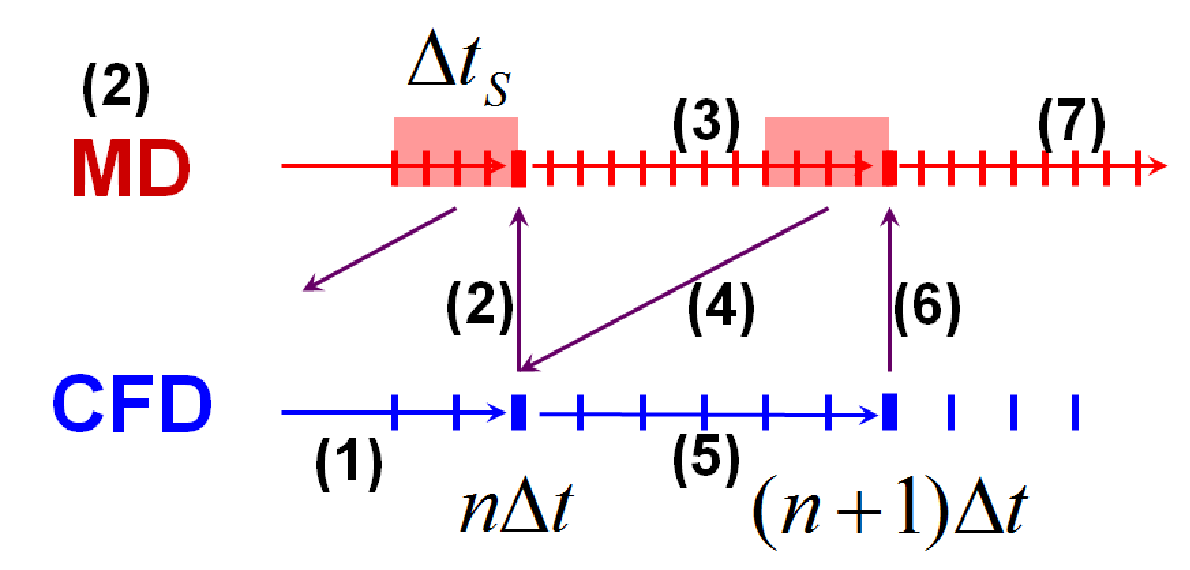
\includegraphics[width=0.8\linewidth]{Sequential_Coupling.pdf}
%\vskip-0.2cm
%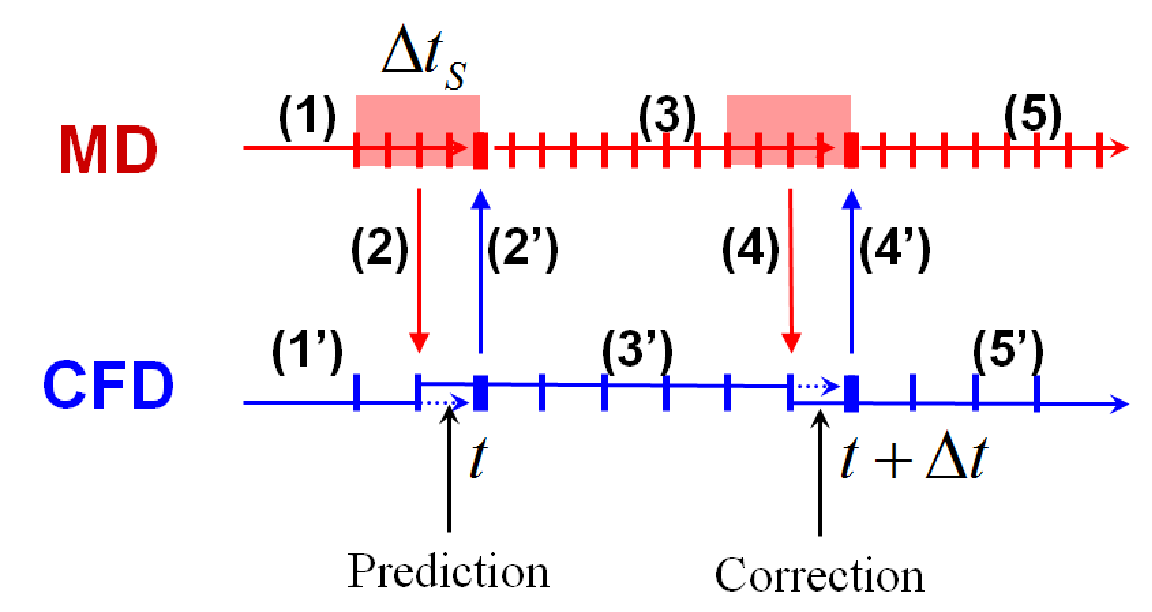
\includegraphics[width=1.0\linewidth]{Prediction_Correction_Coupling.pdf}
\vskip-0.2cm
\caption{\small Conventional Time Evolution Mechanisms of a Hybrid CFD-MD Approach; CFD and MD codes are scheduled to conduct data exchange in the overlapping region at every $\Delta{t}$ sampling interval. CFD solution at $n{\Delta}t$ is directly applied as the boundary condition for MD simulation and backward time-averaged molecular dynamic properties over $\Delta{t_{S}}$ sampling durations are imposed as CFD boundary conditions. (1) Synchronized Coupling: Both codes communicate at the same time level and independently iterate to next exchange point. (2) Sequential Coupling: From the same time level, one solver advances to the next communication point and impose implicit boundary condition to its counterpart.}
\label{Hybrid_Timescale1}
\end{figure}


%Time-lagging phenomenon in CFD boundary region is observed in both strategies, because averaged molecular dynamic properties over backward sampling duration (from $n{\Delta}t-{\Delta}t_{s}$ to $n{\Delta}t$) are used to impose the CFD boundary condition at that instance ($n{\Delta}t$). Thus, the extrapolation from previous MD solutions is necessary to eliminate the time-lagging by half of sampling duration (${\Delta}t_{S}/{2}$) in the CFD boundary zone which is accumulated at every sampling interval.
As is presented in Fig.~\ref{Hybrid_Timescale2}-(0), Wang and He~\cite{Wang} proposed shifting the time axis of one domain by half of the sampling interval to eliminate this lagging effect. After both codes evolve by a sampling interval, the instantaneous CFD solution at $n{\Delta}t$ is communicated with averaged MD solution from $(n-1/2){\Delta}t$ to $(n+1/2){\Delta}t$. Two previous solutions from the counterpart are extrapolated to impose hybrid boundary conditions. The benefit of imposing extrapolated boundary condition is that the sampling duration can be designed as long as the sampling interval (${\Delta}t_{s}={\Delta}t$). However, the accuracy of extrapolated solution is worth to debate. In this scheduling, two \textit{previous} CFD solutions at $(n-1){\Delta}t$ and $n{\Delta}t$ are extrapolated to produce MD boundary conditions from $(n+1/2){\Delta}t$ to $(n+3/2){\Delta}t$. Except the velocity gradient is linear in time space, extrapolated properties fail to predict correct values throughout the simulation interval (from$(n+1/2){\Delta}t$ to $(n+3/2){\Delta}t$). The only way to reduce this extrapolation error is to reduce the sampling interval, which is contradictory to the condition for reducing the statistical error.


\begin{figure}
\centering
%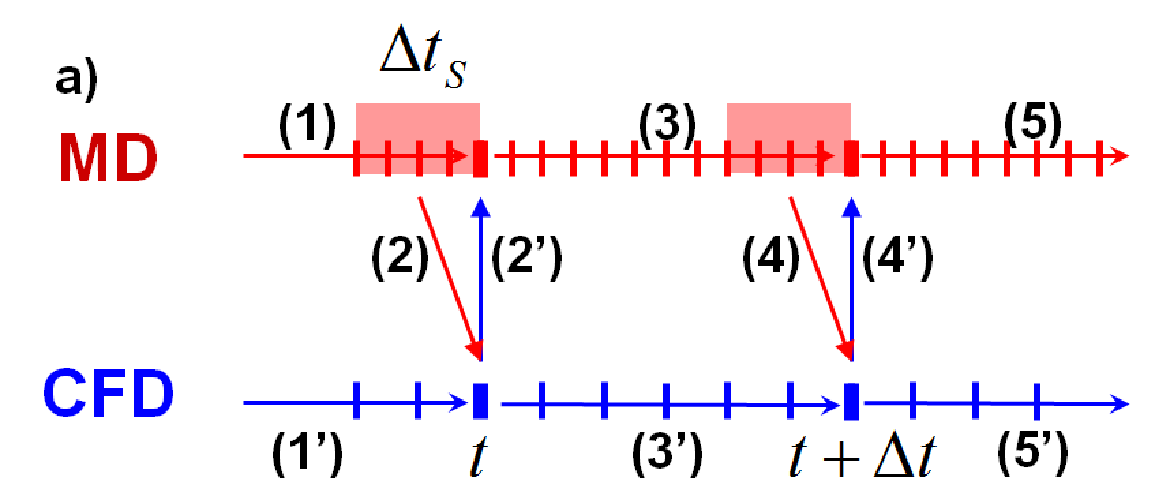
\includegraphics[width=1.0\linewidth]{Synchro_Coupling.pdf}
%\vskip-0.2cm
%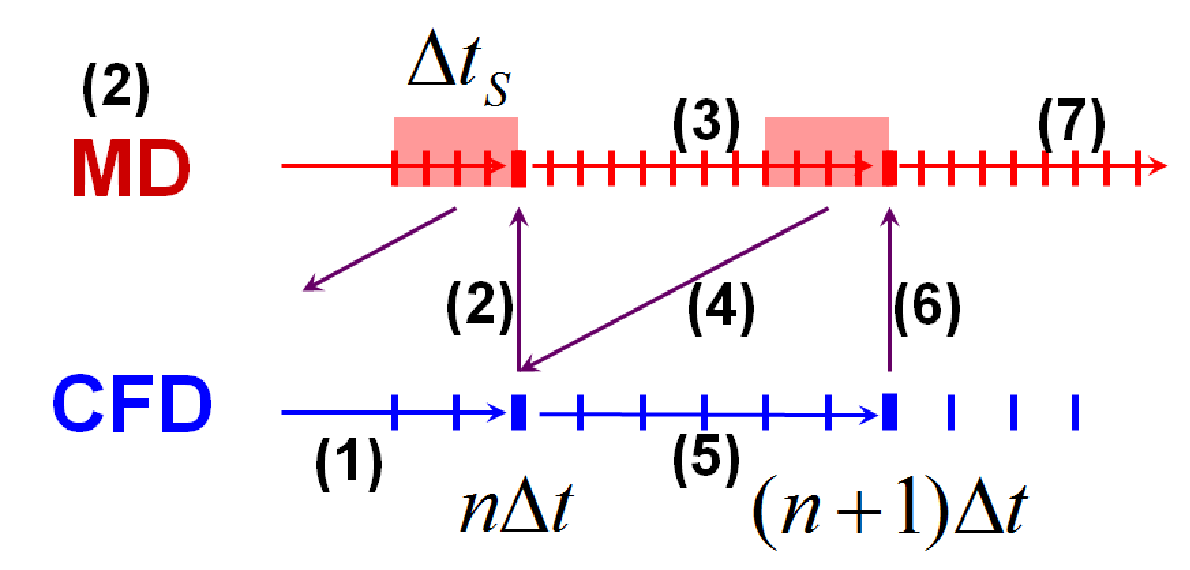
\includegraphics[width=1.0\linewidth]{Sequential_Coupling.pdf}
%\vskip-0.2cm
%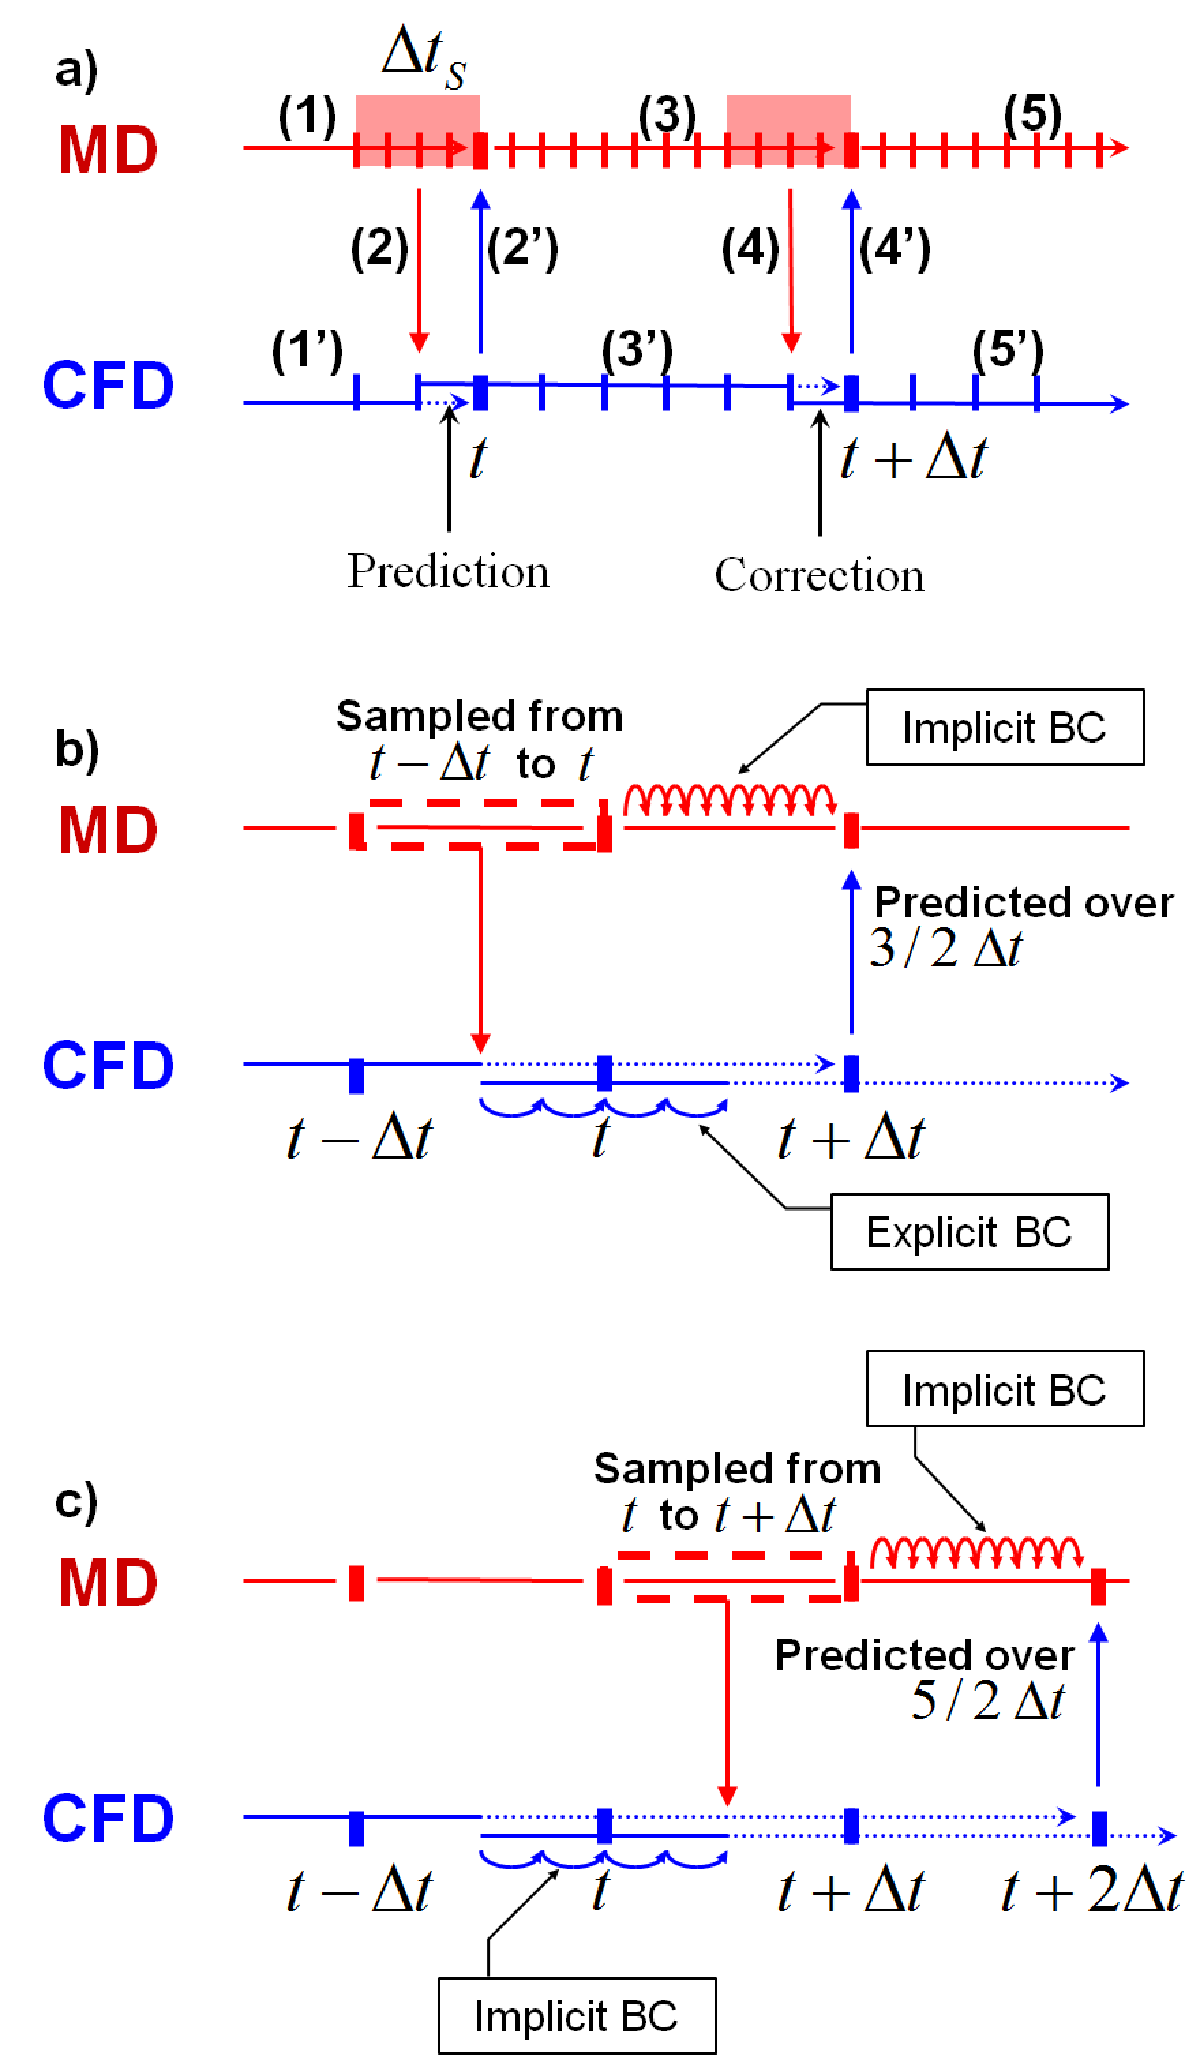
\includegraphics[width=0.6\linewidth]{Prediction_Correction_Full.pdf}
%\vskip-0.2cm
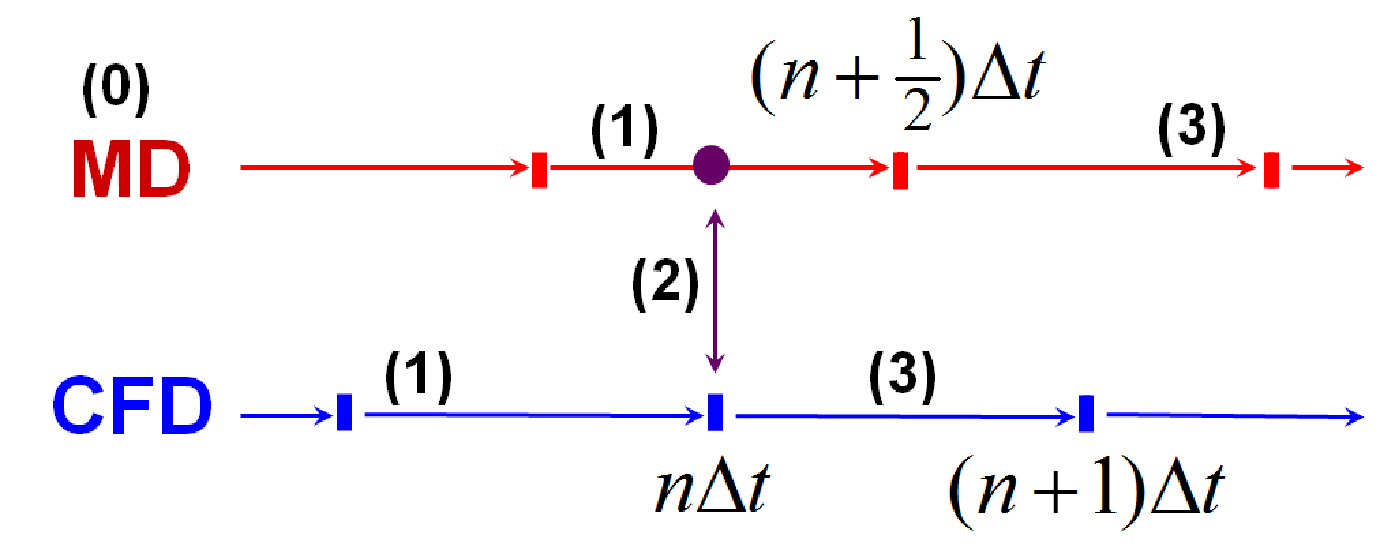
\includegraphics[width=0.7\linewidth]{Prediction_Correction_Org.pdf}
%\vskip-0.2cm
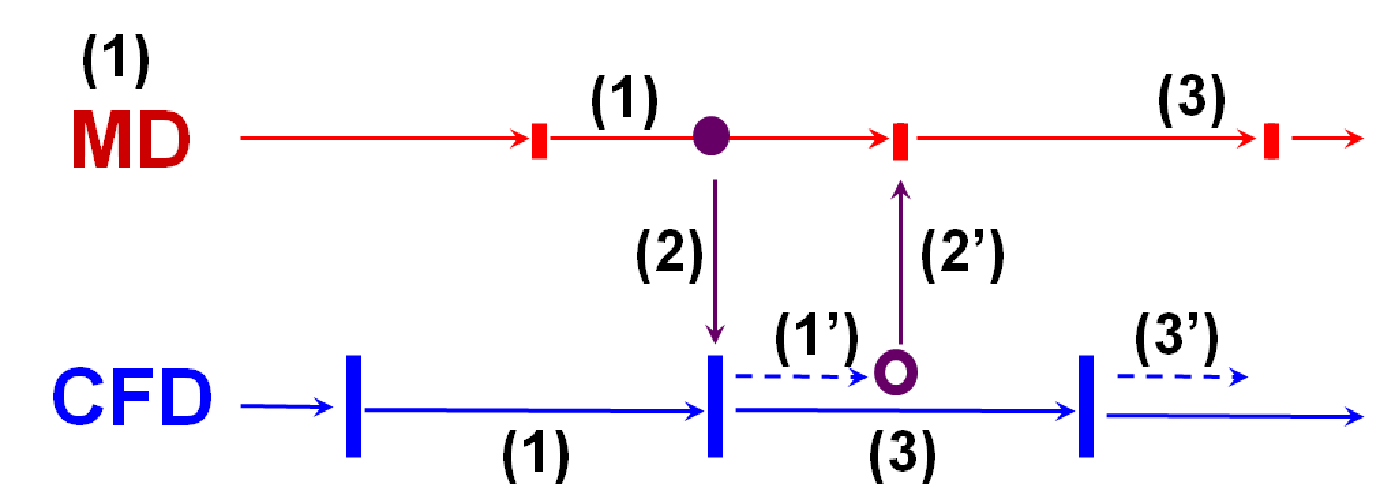
\includegraphics[width=0.7\linewidth]{Prediction_Correction_Extra_Simple.pdf}
%\vskip-0.2cm
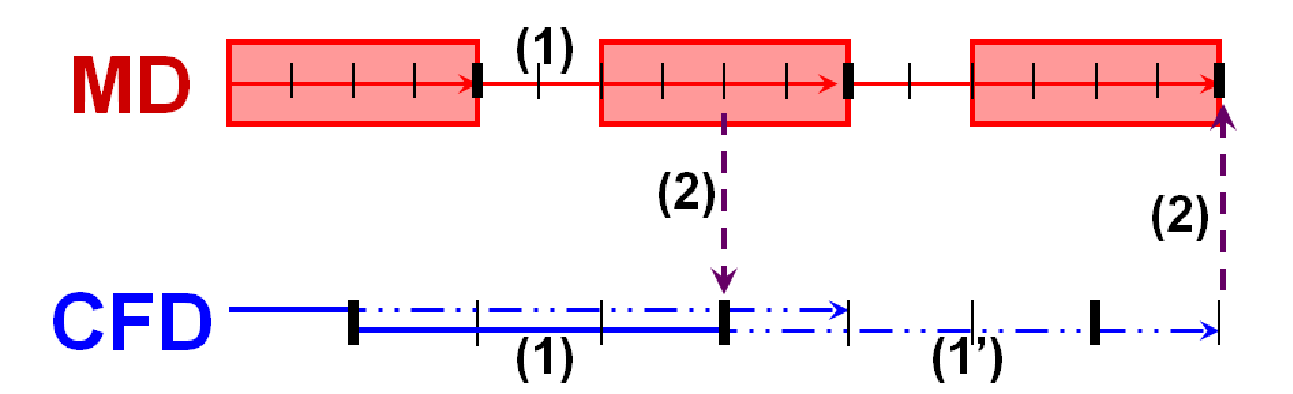
\includegraphics[width=0.7\linewidth]{Prediction_Correction_Inter_Simple.pdf}
%\vskip-0.2cm
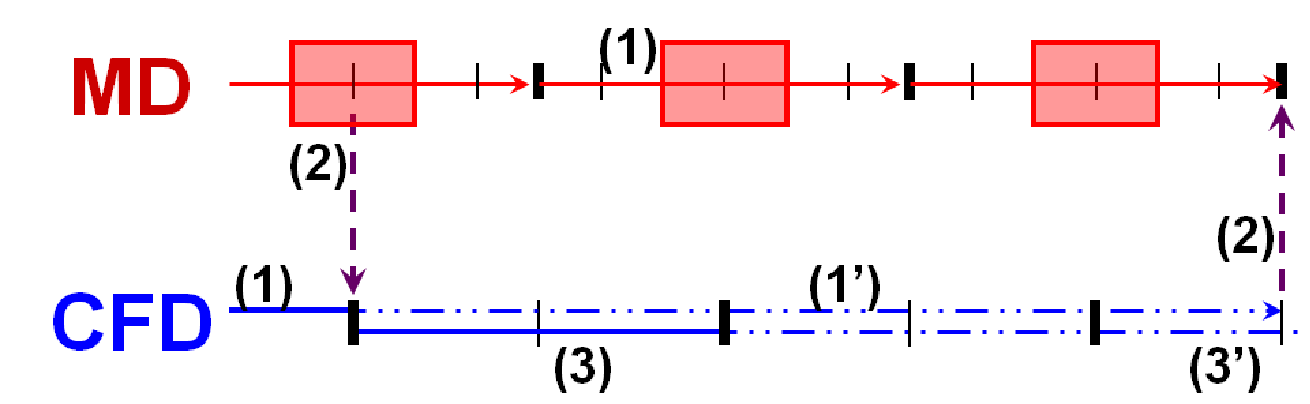
\includegraphics[width=0.7\linewidth]{Prediction_Correction_Both_Simple.pdf}
\caption{\small A Prediction-Correction Approach with Extrapolated/Interpolated Hybrid Boundary Conditions; Applying extrapolation/interpolation enables increasing sampling duration as long as sampling interval. (0) Default Formulation;
%CFD code experiences extrapolated hybrid BC from the current MD solution, while MD code imposes the extrapolation from previous solutions by half of the sampling interval.
The hybrid BC in MD code is extrapolated from previous solutions.
% by half of the sampling interval.
(1) Extrapolated Boundary; CFD code runs the prediction step by $0.5{\Delta}t$. MD code imposes the hybrid BC by the extrapolation from the current value. (2) Interpolated MD Boundary; CFD code runs the prediction step by $1.5{\Delta}t$. MD code imposes interpolated hybrid BC. (3) Interpolated Hybrid Boundary Conditions; Time axis of CFD domain shifts back by 1 sampling interval and the prediction step is set $2.5{\Delta}t$. CFD and MD domains impose interpolated hybrid BC.}
\label{Hybrid_Timescale2}
\end{figure}


% The basic pattern of our approach is the same as the synchronized coupling. Main difference is, CFD code loads the previous solution at $t-{\Delta}t_{S}/{2}$ after communicating with MD code at $t$ and restarts the computation to the next communication point of $t+{\Delta}t$. Thus, time interval between $t - {\Delta}t_{S}/{2}$ and $t$ gets to be solved twice: first in prediction step and second in correction step. Clear benefit of current approach is that time-lagging problem is resolved without numerical treatments and additional computational overhead is acceptable because usually computational cost in MD simulation is dominant for a coupled simulation.
A new scheme named `prediction-correction approach' is also depicted in Fig.~\ref{Hybrid_Timescale2}. The main difference from the default model is that CFD code iterates additional  time steps after the code evolved to the next data exchange time. For example, in Fig.~\ref{Hybrid_Timescale2}-(1), CFD code additionally evolves by the half of sampling interval after the code approached to $n{\Delta}t$. CFD code sends these predicted properties at $(n+1/2){\Delta}t$ to the MD site and receives averaged molecular properties around $n{\Delta}t$. CFD code loads its previous flow profile at $n{\Delta}t$ and runs the actual simulation to next communication point at $(n+1){\Delta}t$. Clear benefit of current approach is that both solvers extrapolate their boundary conditions from \textit{current} solutions (either exact solution or predicted values) instead of using \textit{previous} history. This eliminates the sensitivity of extrapolated solution according to the size of sampling interval in previous model, which enables increasing the sampling interval.

This approach is further refined to increase the accuracy of the hybrid boundary condition by increasing prediction time scale. In Fig.~\ref{Hybrid_Timescale2}-(2), the prediction time scale is increased by one more sampling interval. While MD solver evolves for one sampling interval, CFD code iterates to the next communication point of MD time space. This enables MD boundary condition being interpolated by predicted CFD profiles. Figure ~\ref{Hybrid_Timescale2}-(3) demonstrates the imposition of interpolated boundary conditions on both domains. In this formulation, CFD time space is shifted backward by one sampling interval and prediction step is scheduled to be $(5/2){\Delta}t$.


%A new approach named `prediction-correction strategy' is depicted in Fig.~\ref{Hybrid_Timescale2}. After the data exchange at $t$, MD advances to the next communication point by extrapolating two previous boundary conditions at $t-\Delta t$ and $t$. On the other hand, CFD code loads the previous solution at $t-{\Delta}t_{S}/{2}$ after communicating with MD code at $t$ and evolves to $t+{\Delta}t$ by imposing extrapolated boundary condition from data at $t-\Delta t - {\Delta}t_{S}/{2}$ and $t-{\Delta}t_{S}/{2}$, which makes the difference from the original strategy. In this approach, time interval between $t - {\Delta}t_{S}/{2}$ and $t$ gets to be solved twice: first in prediction step and second in correction step. Clear benefit of current approach is that both solvers are provided with the ``exact" boundary condition once in every sampling interval, compared to the original formulation in which boundary condition had to be extrapolated ``everytime" or the quasi-steady assumption had to be satisfied. As the exact boundary condition is provided at every sampling interval, sampling duration can be increased as long as sampling interval, which will reduce statistical error. Furthermore, with longer prediction setting as seen at Fig.~\ref{Hybrid_Timescale2}-b) and c), more accurate boundary condition can be imposed by simulating over longer prediction time.


Current numerical approach provides more accurate time-variant solution by decreasing or eliminating the unfavorable overshoot/undershoot phenomena in extrapolations. Meanwhile, additional computational cost is inevitable for CFD simulation. We propose the current approach to be used in following conditions: (i) computational cost on CFD is quite smaller than that of MD, and (ii) the driving force which causes the flow variation is provided from the CFD domain. Without condition (i), additional computational overhead for prediction process will harm the simulation performance. If (ii) is not satisfied, the pattern of flow evolution cannot be predicted and the accuracy of the predicted solution is not guaranteed.



\section{Coupled Concurrent Multi-Scale (Continuum-Molecular) Simulation Framework}
\label{sec:computational}

Two important issues on the performance of hybrid simulations are co-scheduling and load-balancing. Both can be resolved by adopting a Pilot-job concept. We explain the design of a multi-physics simulation framework which operates in the form of a single Pilot-job and contains a load-balancing function between distinct tasks.

\subsection{SAGA and SAGA-based Frameworks - An Efficient Runtime Environment for Coupled Multi-component Computations}

The Simple API for Grid Applications (SAGA) is an API standardization effort within the Open Grid Forum (OGF)~\cite{ogf_web}, an international standards development body concerned primarily with standards for distributed computing. SAGA provides a simple, POSIX-style API to the most common Grid functions at a sufficiently high-level of abstraction so as to be independent of the diverse and dynamic Grid environments. The SAGA specification defines interfaces for the most common Grid-programming functions grouped as a set of functional packages (Fig.~\ref{Fig:SAGA1}). Some key packages are:

\begin{figure}
 \begin{center}
     \includegraphics[width=0.8\textwidth]{Structure_of_SAGA.eps}
 \end{center}
\caption{\small Layered schematic of the different components of the SAGA landscape. At the topmost level is the simple integrated API which provides the basic functionality for distributed computing. Our BigJob abstraction is built upon this SAGA layer using Python API wrapper}
 \label{Fig:SAGA1}
 \vspace{-1em}
\end{figure}

\begin{itemize}
\item File package - provides methods for accessing local and remote filesystems, browsing directories, moving, copying, and deleting files, setting access permissions, as well as zero-copy reading and writing
\item Job package - provides methods for describing, submitting, monitoring, and controlling local and remote jobs. Many parts of this package were derived from the largely adopted DRMAA %~\cite{drmaa_url} specification.
\item Stream package - provides methods for authenticated local and remote socket connections with hooks to support authorization and encryption schemes.
\item Other Packages, such as the RPC (remote procedure call) and Replica package
\end{itemize}


%\skonote{Introduction to BigJob and related researches from other researchers: show their limitation as well - i.e., LB issue, etc.. Include REMD, co-scheduling of multiple tasks via SGE in Ranger. 2 paragraphs. I'd like to include "SAGA enables creation of higher levels of abstraction, such as a container-job or a Pilot-Job (which, as we will discuss, is referred to as the BigJob~\cite{saga_royalsoc}). The SAGA-based Pilot-Job is infrastructure neutral, unlike {\it all} other Pilot-Jobs."}

%\skonote{Exclude the mention about the multiple BigJobs. Also, focus on explaining BigJob's advert service module in detail, including referring to Andre's paper}

The BigJob~\cite{saga_royalsoc} is a SAGA-based Pilot-Job, where a number of sub-tasks can run in a pre-defined schedule with the specified number of processors whether or not they are coupled. We basically devise this solution to overcome the concurrent scheduling requirement of coupled CFD and MD jobs and to dynamically allocate resources for load-balancing of these codes. The advantage of a BigJob over other Pilot-Job implementations is that this is infrastructure-neutral, thanks to various adaptors in SAGA.


Fig.~\ref{Fig:BigJob_Structure} shows the structure of BigJob and its operation flow. When a BigJob is submitted to the remote resource, the application manager monitors the status of this Pilot-Job through the advert service. When resources are allocated to the BigJob, the application manager allots the obtained resources to its sub-jobs and a coupled simulation starts under the control of a multi-physics agent in the remote resource. Advert service keeps on getting the status of a Pilot-Job from the queuing system and the status of sub-jobs from multi-physics agent. It also delivers this information to the application manager by a push-pull mechanism. The application manager watches the status of sub-jobs and decides the next event when the coupled simulation is finished. If an individual simulation is of interest, the manager closes a BigJob allocation when the simulation is finished: In cases of multiple replica simulations or load-balanced coupled simulation, the manager relaunches sub-jobs on the same BigJob allocation until all replicas or load-balancing steps are completed.
% experience pre-designed several launches on the same BigJob allocation until the whole simulation is completed.


%%%%% FIGURE %%%%%
\begin{figure}
\centering
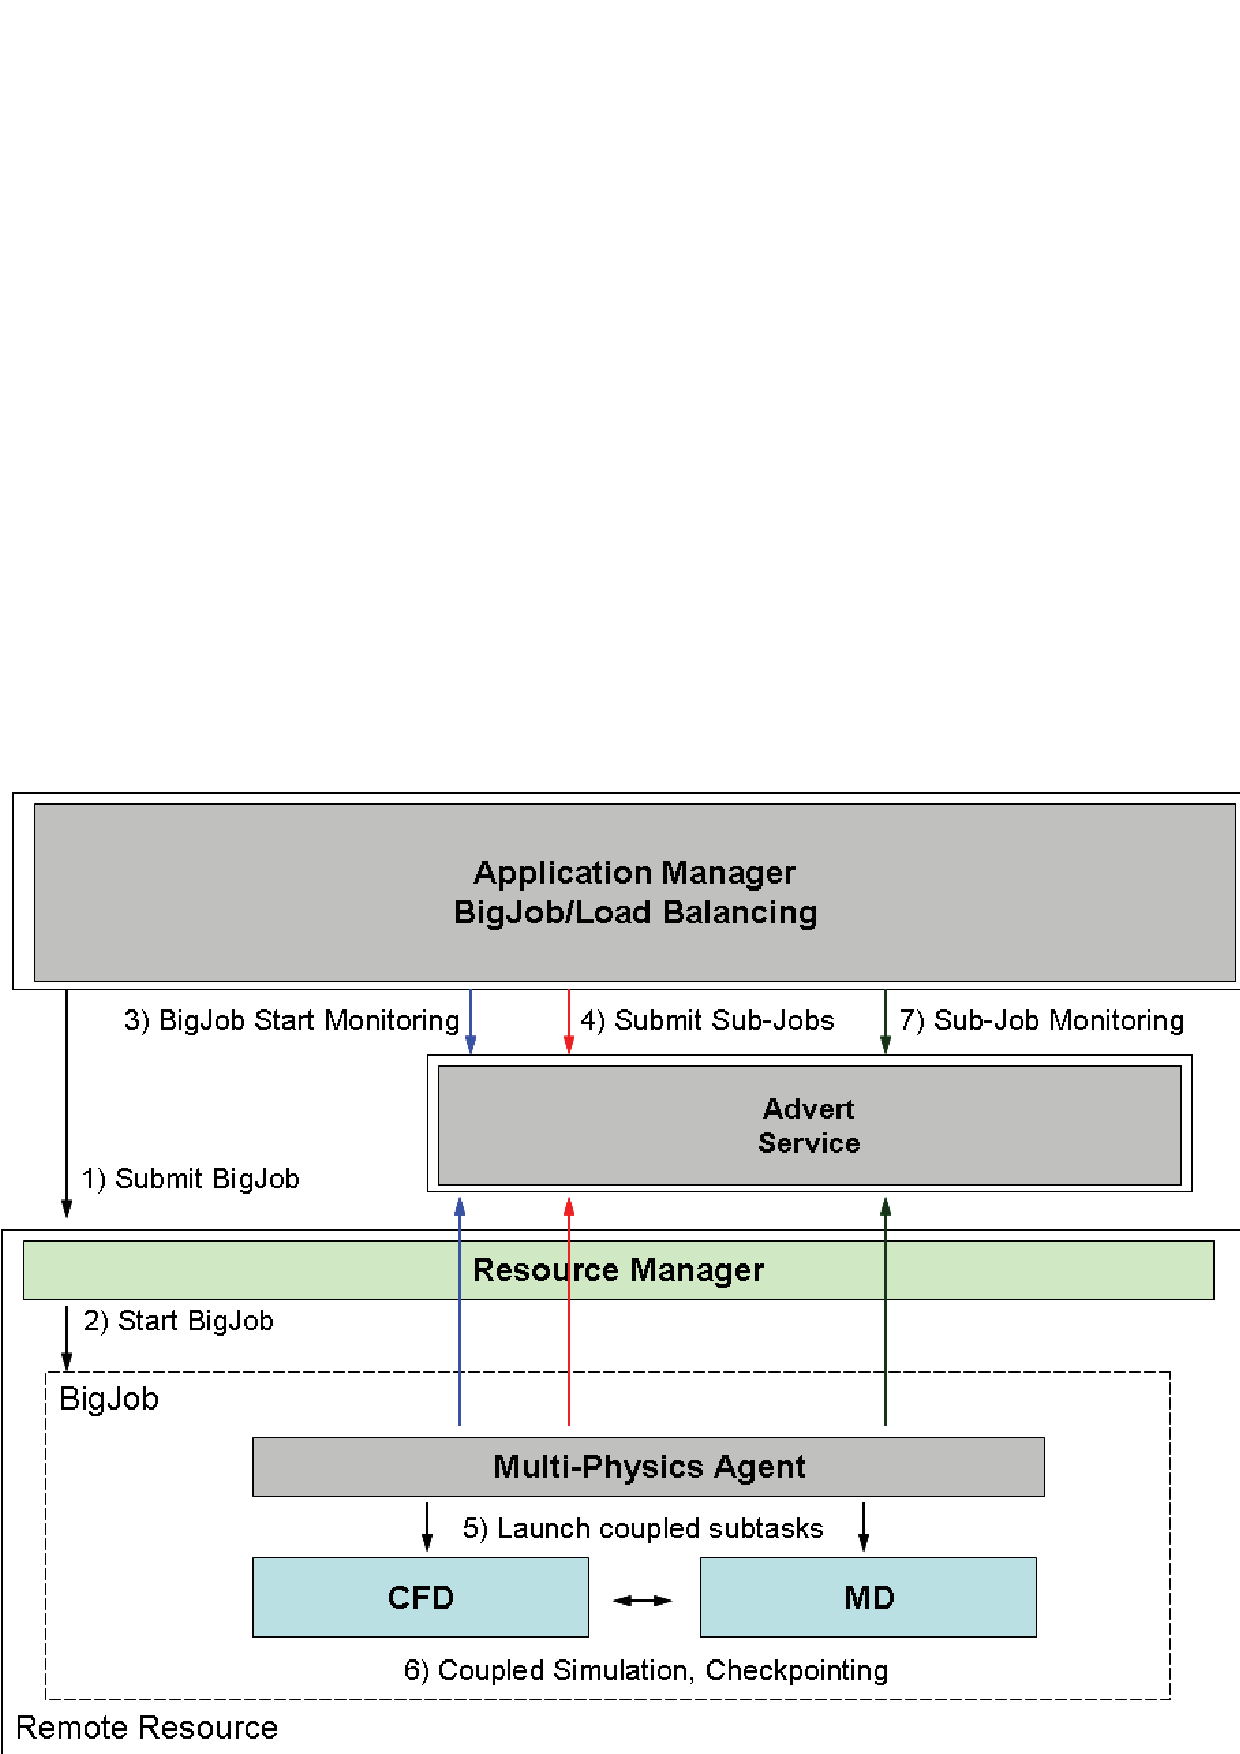
\includegraphics[width=0.8\linewidth]{Structure_of_BigJob}
\caption{\small Architecture of the Controller/Manager and Control Flow: Application manager is responsible for job management including BigJob and sub-job submission, their status monitoring functions. We implement a load-balancing module, and migration service based on job information. Application agent system resides on each HPC resource and conducts job information gathering and also communicates with the application manager via the advert service}
\label{Fig:BigJob_Structure}
\vspace{-1em}
\end{figure}
%%%%% FIGURE %%%%%


\subsection{Load-Balancing of Coupled Multi-Physics Simulation}
Load balancing of a coupled simulation implies the flexibility to re-distribute resources to the individual task according to the performance of individual job. We will discuss the implementation and algorithm of a simple load balancer (LB)~\cite{Ko}; it is important to mention that the LB functions in the context of the SAGA-BigJob framework.

The idea is to assign more resources to heavier sub-jobs under the fixed resource allocation, until all sub-jobs elapse the same execution time. As it is impossible to predict the performance of each code in advance, we let the LB monitor the wall-clock time between information exchange points of coupled tasks and iteratively change the processor distribution until the load balancing is achieved. As the individual solver is considered as black-box, each application code is assumed to have the ideal parallel efficiency: In case application codes are highly scalable, the LB can find the best condition after a few dynamic re-distributions. Also, all processors in one node are assigned to one single task to prevent the interference when multiple MPI tasks are running in a single node.\skonote{I found that the performances of MPI jobs decrease if more than two codes share a single node. For example, two 4-px jobs run at the same node of queenbee, performance of each code is half of one 4-px job: two codes share the same 4 processors and another 4 processors are idling. That's the same on Ranger. Looks as if the problem of default MVAPICH configuration, as I saw the same problem in KISTI.}


%Each application's load is determined by its elapsed time to run the evolution loop. Here, time for initialization or inter-domain data exchange are excluded from the counting, because they are one-time events or irrelevant to application's performance. The efficient functioning of the LB is predicated on application codes being able to restart from their checkpointing data effectively.  Also, application codes should be equipped with generalized domain partitioning routine to run a simulation with any number of processors, without harming their parallel efficiency a lot. If above conditions are satisfied, it makes sense to load the LB within the Pilot-Job, to implement dynamic resource allocation between tasks.  Conceptually, the load-balancing algorithm assigns more processors to a sub-task with greater runtime, until the two codes take the same wall-clock time between points when they communicate. Interestingly, our approach is very simple and the algorithm is independent of applications upon the predications of,
%(1) each application code follows the ideal parallel efficiency.
%(2) all processors in one node are assigned to one single task.


Let the computation time (between exchanges) of the two sub-jobs be $t_{CFD}$ and $t_{MD}$, and the number of processors assigned to each domain be $PE_{CFD}$ and $PE_{MD}$, respectively. Subscripts C and N denotes current and next states. Assuming ideal parallel efficiency, total load of each application remains the same after resource re-allocation,

\vspace{-.2em}
\footnotesize
\begin{eqnarray}
W_{CFD}&=&PE_{CFD,C}\times t_{CFD,C}=PE_{CFD,N}\times t_{CFD,N} \nonumber \\
W_{MD}&=&PE_{MD,C}\times t_{MD,C}=PE_{MD,N}\times t_{MD,N}
\label{eq:SimTime_EachTask}
\end{eqnarray}
\normalsize

In spite of the re-allocation, the total number of processors utilized remains the same:

\vspace{-.2em}
\footnotesize
\begin{equation}
PE_{TOT}=PE_{CFD,C}+PE_{MD,C}=PE_{CFD,N}+PE_{MD,N}
\label{eq:PECondition}
\end{equation}
\normalsize

Our objective is to reduce the computation time of a sub-job to the point until the two application components show the same computation between the exchange points, i.e., $t_{CFD,N} = t_{MD,N}$. From Eqn.~\ref{eq:SimTime_EachTask} and Eqn.~\ref{eq:PECondition} an optimal number of processors distributed for the CFD subtask would be:

\vspace{-.2em}
\footnotesize
\begin{eqnarray}
PE_{CFD,F} & = & \frac {W_{CFD}} {(W_{CFD} + W_{MD})} \times PE_{TOT}
\end{eqnarray}
\normalsize

The MD simulation (sub-job) will follow a similar expression.
%The optimal processor distribution from above equation will return a non-integer value. Also, under the second assumption (which is the policy of many supercomputing centers), any load-balancing determined as above, will proceed in discrete values expressed as the multiples of the number of CPU cores in a node. We choose the nearest discrete number to our load-balancing as the optimal number of processor on each application.

The above non-integer value proceed in discrete values expressed as the multiples of the number of CPU cores in a node. We choose the nearest discrete number to our load-balancing as the optimal number of processor on each application.


%\skonote{Based on Section 4 in CCGrid 2010: Refine LB, include motivation etc. (e.g., Not touching application codes)\\
%refined LB algorithm is going to be,\\
%\begin{equation}
%c_{2} \times PE^{2} + c_{1} \times PE^{1} + c_{0} \times PE^{0} + c_{-1} \times PE^{-1}
%\end{equation} \\
%Where $c_{0}$ is serial term, $c_{-1}$ would be related to pure computation, communication is somewhat influencing $c_{0}$ and $c_{1}$ if communication size is small enough that it is only the latency-related value (thus would be constant) and global communication time is proportional to the number of processor, also considering the waiting time affecting $c_{1}$ and $c_{2}$, which is proportional to the total number of processors and additional overhead is considered as the second order term\\
%In cases more refinements are needed, use the following:\\
%1. Total Time for One Simulation = f(serial) + f(pure computation) + f(inter-proc.comm) + f(global.comm) + f(waiting)\\
%2. Serial part of the code as $c_{serial}$\\
%3. Pure computation part is $c_{comp} \times PE^{-1}$ - Total computation size remains the same regardless of number of processors\\
%4. Communication pattern 1: inter-processor BC communication, it depends on whether the problem is 1-D, 2-D or 3-D: \\
%in 1-D, it is $c_{comm1D}$ as only point vales exchange\\
%in 2-D, it is $c_{comm2D} \times PE^{-1/2}$\\
%in 3-D, it is $c_{comm3D} \times PE^{-2/3}$\\
%5. Communication pattern 2: global communication, 0th processor will communicate with all processors, usually communication size is the same (maybe an integer value is communicated), so the time is $c_{global.comm} \times PE^{1}$ \\
%6. Waiting time: unclear, but would likely be proportional to inter-processor communication time multiplied by the total number of processors, so\\
%$c_{wait} \times f(inter-proc.comm) \times PE^{1}$ \\
%\newline
%After the modeling, apply it on CFD and MD simulations (separate simulations on three different system sizes) and include the graph. Also needs some comment like \\
%'there's no general LB for any programs 'cause it's usually based on the programming skills, e.g., how to use optimal compilation option for the system, how low the cache miss takes place, etc. Thus, regarding the pure computation, it is not inversely proportional to the number of processors as the reference to cache memory dramatically increases if problem size to each processor becomes sufficiently small.'\\
%Also mention that this needs numbers of evolution loops to go to the final solution. In the first case, 4 for finding all coefficient values and 5 for %next one.}



\subsection{Implementation of an Execution Framework and Application-level Corrections}

A hybrid CFD-MD framework is evaluated by implementing an application manager in Fig.~\ref{Fig:BigJob_Structure}, which is written in PYTHON script language. By default, an application manager calls a number of SAGA functions in sequence, to get allocated a vacant job, to run individual MPI simulation, to monitor its status, and to finalize the BigJob allocation.

In case the load-balancing capability is turned on, the situation becomes complicated. A single MPI job is not able to change its number of processors during the simulation. This implies that coupled codes should stop-and-restart to get assigned with changed number of processors. Thus, sub-jobs are scheduled to have multiple restarts from the previous checkpointing solution, which we denote 'load-balancing steps'. A LB is provided as a separate function in an application manager and is scheduled to run in between each restart of sub-jobs.

The efficient functioning of the LB is predicated on application codes being able to restart from their checkpointing data effectively. Application codes should also be equipped with generalized domain partitioning routine to run a simulation with any number of processors, without harming their parallel efficiency a lot.
Another change implemented on application codes is the time checking routine. The runtime of each application is meaningless in running a LB since this runtime contains idle waiting on inter-domain information exchange as well as the individual computation time. This actual runtime can be counted by putting two wall-time functions before and after the information exchange routine.


The generation of an application manager and the changes in application codes raise the possible simulation scenarios as given in Fig.~\ref{Fig:OneBJ_Flow}. The first (leftmost) shows the time evolution of a coupled simulation under a conventional job submission (which we define to be scenario S0), and others using a BigJob (denoted as S1). For S0, individual tasks with resource requirements of $PE_{CFD}$ and $PE_{MD}$ respectively, are independently submitted to the conventional queuing system and job scheduler recognizes these coupled tasks as two distinct jobs. Thus, they start at different times on average.
%except when coincidentally resources for both are available.
In this case, both tasks wait on the queue when no job is allocated (waiting stage), the first allocated job idles to perform data exchange with its counterpart (idling stage), and the actual simulation starts when both jobs are allocated (running stage). On the other hand, for scenario S1, a BigJob of size $PE_{CFD}+PE_{MD}$ is submitted to the queue, and coupled simulation directly starts when the resource is assigned to this BigJob. Because of co-scheduling of sub-jobs, a BigJob is free from long inactive mode which is frequent in conventional job submission, while total runtime is the same if the resource distribution to sub-jobs is identical. However, eliminating inactive mode in itself does not guarantee a reduction in the total runtime, because a larger single allocation may result in a greater queue waiting time than two simulations requesting smaller number of processors each (but the total being the same). The same situation can arise for the load-balanced case with one BigJob ($S1_{LB}$). From the comparison between S1 and S0, we can estimate the performance gain by concurrent start of distinct coupled codes; $S1_{LB}$ solution compared to other scenarios will demonstrate the benefit of a load-balancing function on coupled simulation.


%%%%% FIGURE %%%%%
\begin{figure}
%\vspace{-1em}
\centering
%\includegraphics[width=0.8\linewidth]{Simulation_Time_of_One_BigJob.eps}
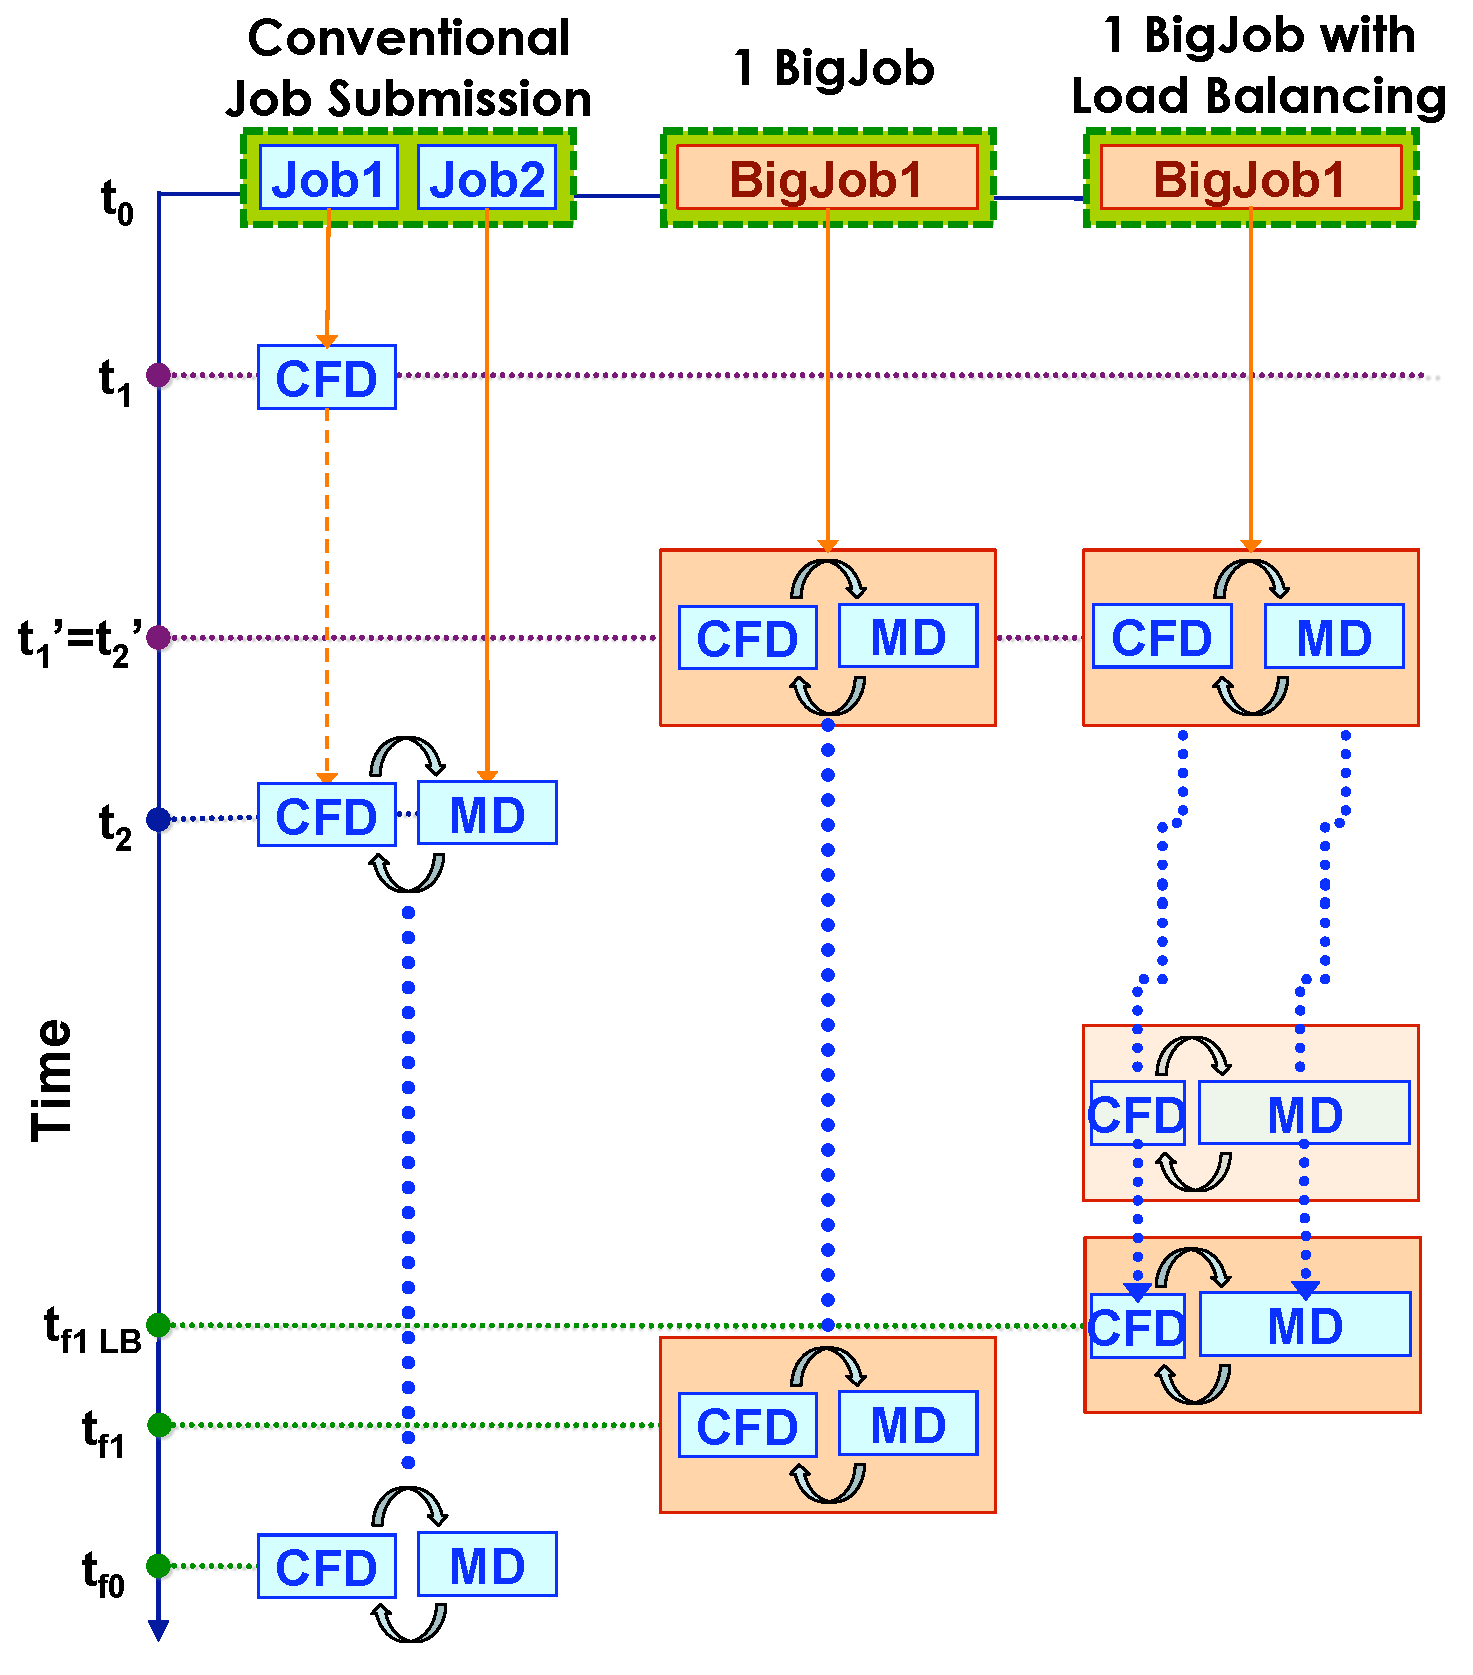
\includegraphics[width=0.8\linewidth]{Single_BigJob_Scenarios_new.pdf}
\caption{\small Comparison of dependencies encountered for coupled
  simulations submitted as conventional jobs, to the scenario when
  using Pilot-Jobs. Here we use only 1 BigJob (S1). The conventional
  mode of submission experiences three phases based upon their queue
  state: (i) All jobs are waiting: ($t_1-t_0$); (ii) Inactive mode
  (where one job is waiting for another: $t_2-t_1$), and (iii) Active
  mode (running a coupled simulation: $t_f-t_2$). The Inactive stage,
  disappears when a coupled simulation runs within a BigJob, as an
  allocated BigJob distributes its resource to both sub-jobs.}
\label{Fig:OneBJ_Flow}
\vspace{-1em}
\end{figure}
%%%%% FIGURE %%%%%



\section{Multi-physics Flow Simulations in Various Flow Conditions}
\label{sec:accuracy}
A hybrid CFD-MD framework is employed to solve the multi-physics flow in nano-scale. Experimented problems are a sudden-start Couette flow and the oscillating boundary problem. We start from determining coupling parameters to the validation and verification of the hybrid simulation framework, then to the exploration of the moderate-speed flow simulation and time-accurate hybrid simulation.

\subsection{Problem Description and Coupling Conditions}
\label{sec:accuracy_conditions}

All applications we examine are internal flow fields filled with the liquid argon. Characteristic length of liquid argon is ${\sigma}=3.405{\times}10^{-10}$ and time scale is $\tau=2.2{\times}10^{-12}$. Density is $0.81m{\sigma}^{-3}$, which means 0.81 atoms are included in the characteristic volume.
The fluid domain is a channel system which consists of two parallel plates placed in vertical direction. Liquid argon particles are filled in the domain and both walls have artificial properties which is the same as those of liquid argon. The slip ratio between fluid and solid particles are set 0.6, to satisfy the linear velocity gradient along the vertical direction.~\cite{Nie}
%Channel height is set to In view of system size, two fluid systems are solved in our experiments, i.e., 10$^{-8}$ (52 $\sigma$) and 10$^{-7}$ (520 $\sigma$) meters in the height of channel. Applications covered in this work are periodic systems in the perpendicular direction and the flow variation is derived by the horizontal motion of an upper plate.
Channel is 52 $\sigma$ in height, which is O(10$^{-8}$) meters. Applications covered in this work are periodic systems in the perpendicular direction and the flow variation is derived by the horizontal motion of an upper plate.


As has been proposed in Sec.~\ref{sec:numerical_parameters}, we solve a stationary flow in particle domain to determine coupling conditions. Table \ref{table:MD_Vel0} shows the averaged velocity depending on the layer size and sampling duration in 10$^{-8}$ meter domain. Experiments were conducted with different lengths of the domain, changing from 35 $\sigma$ to 70 and 140 $\sigma$. Noises around 0.2 height above the wall are presented.

From the individual test, we find that mathematical expressions on the strength of noise according to the height of sampled layer and sampling duration~\cite{Hadjicon3,Time_Mechanism} do not coincide with our experiment. From the first table, increasing the height of averaged layer from 0.1 to 6.4 $\sigma$ reduces the statistical error by 4 times when sampling duration is 1 $\tau$ and this ratio even gets worse as sampling duration increases. The same situation also happens on sampling duration.
%From the individual test, we find that increasing sampling duration or height of averaged layer does not linearly decrease the statistical error. At the first test, increasing the height of averaged layer from 0.1 to 6.4 $\sigma$ reduces the statistical error by 4 times when sampling duration is 1 $\tau$ and this ratio even gets worse as sampling duration increases. The same situation also happens on sampling duration.
This is contradictory to previous mathematical expressions which has been introduced in Sec.~\ref{sec:numerical_noise}.
%, where noise is inversely proportional to the root of layer height or sampling interval and these two factors are not coupled.
From the data analysis, we figure out that the magnitude of sampling noise depending on the layer size and sampling duration is far more complicated: $V_{N} = a \times SD^b \times LH^c \times SD^{d \times ln(LH)}$, where $V_N$ represents the velocity magnitude of the noise, $SD$ denotes sampling duration and $LH$ is the height of the layer.
%The mathematical expression on the strength of noise depending on the layer size and sampling duration is far more complicated than have been addressed in previous analyses: $V_{N} = a \times SD^b \times LH^c \times SD^{d \times ln(LH)}$, where $V_N$ represents the velocity magnitude of the noise, $SD$ denotes sampling duration and $LH$ is the height of the layer.
This equation is rewritten in simpler logarithmic formulation as,

\vspace{-.2em}
\footnotesize
\begin{eqnarray}
ln(V_{N}) = ln(a) +b~ ln(SD) +c~ ln(LH) +d~ ln(SD)~ ln(LH)\nonumber
\label{eq:Noise1}
\end{eqnarray}
\normalsize
and these coefficients in our specific case are as,


\vspace{-.2em}
\footnotesize
\begin{eqnarray}
&L = 35 \sigma :   &a = 33.67,~b= - 0.18,~c= - 0.30,~d=0.052\nonumber \\
&L = 70 \sigma :   &a=25.85,~b=- 0.19,~c= - 0.27,~d=0.062\nonumber \\
&L = 140 \sigma : &a=17.78,~b= - 0.18,~c=-0.25,~d=0.060\nonumber
\label{eq:Noise2}
\end{eqnarray}
\normalsize
which directly expresses that 4 times longer sampling duration or 4 times larger layer height is far insufficient to half the noise.

%\vspace{-.2em}
%\footnotesize
%\begin{eqnarray}
%L = 35 \sigma :   ln(V_{N}) & = & ln(33.67) - 0.18~ ln(SD) - 0.30~ ln(LH) \nonumber \\
%& + & 0.052~ ln(SD)~ ln(LH)\nonumber \\
%L = 70 \sigma :   ln(V_{N}) &=& ln(25.85) - 0.19~ ln(SD) - 0.27~ ln(LH) \nonumber \\
%&+& 0.062~ ln(SD)~ ln(LH) \\
%L = 140 \sigma :   ln(V_{N}) &=& ln(17.78) - 0.18~ ln(SD) - 0.25~ ln(LH) \nonumber \\
%&+& 0.060~ ln(SD)~ ln(LH)\nonumber
%\label{eq:Noise}
%\end{eqnarray}
%\normalsize



% Table formats; h,t,b,p - here,top,bottom,page of floats
%\begin{table}[t]
\begin{table}
  \caption{\small Statistical Error in Stationary Flow Simulation; Pure MD simulations of 35 $\times$ 52, 70 $\times$ 52 and 140 $\times$ 52 ${\sigma}^2$ are conducted. Liquid is bound in Y-direction by upper and lower walls and able to move in X-direction where periodic boundary condition is imposed. Initial data up to 100 $\tau$ are disregarded to provide enough time for minimization. Velocity of particles around the central layer are accumulated over 512 $\tau$ by using {\it{fix-ave-spatial}} function in LAMMPS package and post-processed to get the average velocity at different layer size and sampling duration conditions. Statistical noise becomes about half at 4 times bigger domain. The unit is 1/1000 of non-dimensional MD velocity (1$\sigma$ / $\tau$).}
  \label{table:MD_Vel0}
  \centering
%  \resizebox{0.8\linewidth}{!} {
\footnotesize
  \begin{tabular}{c || c c c c c c c}
\hline
	&	1 $\tau$	&	2 $\tau$	&	4 $\tau$	&	8 $\tau$	&	16 $\tau$	 &	32 $\tau$	&	64 $\tau$	\\
\hline
0.1 $\sigma$	&	62.332 	&	48.396 	&	40.245 	&	35.006 	&	26.761 	&	 21.605 	&	17.617 	\\
0.2 $\sigma$	&	53.821 	&	43.877 	&	36.693 	&	32.067 	&	24.108 	&	 20.874 	&	18.912 	\\
0.4 $\sigma$	&	46.200 	&	38.967 	&	33.122 	&	29.881 	&	24.044 	&	 19.666 	&	18.827 	\\
0.8 $\sigma$	&	40.087 	&	35.490 	&	31.412 	&	28.671 	&	23.949 	&	 20.382 	&	19.255 	\\
1.6 $\sigma$	&	32.455 	&	30.470 	&	27.382 	&	24.405 	&	20.140 	&	 17.494 	&	16.594 	\\
3.2 $\sigma$	&	23.019 	&	21.877 	&	21.072 	&	18.534 	&	16.532 	&	 14.395 	&	13.643 	\\
6.4 $\sigma$	&	16.113 	&	15.754 	&	15.289 	&	14.649 	&	13.459 	&	 12.909 	&	12.858 	\\
%12.8 $\sigma$	&	13.293 	&	13.235 	&	13.065 	&	12.888 	&	12.668 	&	 12.622 	&	12.492 	\\
\hline
\hline
	&	1 $\tau$	&	2 $\tau$	&	4 $\tau$	&	8 $\tau$	&	16 $\tau$	 &	32 $\tau$	&	64 $\tau$	\\
\hline
0.1 $\sigma$	&	44.207 	&	34.909 	&	28.885 	&	23.981 	&	17.466 	&	 12.986 	&	12.630 	\\
0.2 $\sigma$	&	36.675 	&	31.260 	&	25.690 	&	22.203 	&	18.914 	&	 12.341 	&	11.695 	\\
0.4 $\sigma$	&	32.370 	&	28.093 	&	24.062 	&	19.818 	&	17.875 	&	 12.819 	&	11.980 	\\
0.8 $\sigma$	&	29.544 	&	26.477 	&	23.613 	&	19.966 	&	18.261 	&	 13.404 	&	12.521 	\\
1.6 $\sigma$	&	24.729 	&	22.964 	&	21.099 	&	19.111 	&	17.878 	&	 14.058 	&	12.684 	\\
3.2 $\sigma$	&	18.719 	&	18.102 	&	17.111 	&	16.487 	&	15.723 	&	 13.074 	&	12.115 	\\
6.4 $\sigma$	&	12.791 	&	12.596 	&	12.388 	&	12.121 	&	11.723 	&	 10.311 	&	9.536 	\\
%12.8 $\sigma$	&	7.764 	&	7.687 	&	7.560 	&	7.425 	&	7.157 	&	 6.864 	&	6.565 	\\
\hline
\hline			
	&	1 $\tau$	&	2 $\tau$	&	4 $\tau$	&	8 $\tau$	&	16 $\tau$	 &	32 $\tau$	&	64 $\tau$	\\
\hline
0.1 $\sigma$	&	30.578 	&	24.249 	&	19.228 	&	15.659 	&	13.238 	&	 10.163 	&	9.308 	\\
0.2 $\sigma$	&	26.803 	&	21.931 	&	18.138 	&	14.721 	&	11.844 	&	 10.045 	&	8.494 	\\
0.4 $\sigma$	&	23.158 	&	19.426 	&	16.965 	&	13.620 	&	10.759 	&	 9.742 	&	8.355 	\\
0.8 $\sigma$	&	20.055 	&	17.501 	&	15.703 	&	13.378 	&	10.527 	&	 9.796 	&	8.069 	\\
1.6 $\sigma$	&	15.966 	&	14.691 	&	13.486 	&	11.888 	&	9.944 	&	 9.398 	&	8.034 	\\
3.2 $\sigma$	&	12.584 	&	12.144 	&	11.623 	&	10.484 	&	9.755 	&	 9.295 	&	8.376 	\\
6.4 $\sigma$	&	10.243 	&	10.091 	&	9.860 	&	9.662 	&	9.189 	&	 9.059 	&	8.117 	\\
%12.8 $\sigma$	&	7.832 	&	7.795 	&	7.722 	&	7.639 	&	7.515 	&	 7.471 	&	6.634 	\\
\hline
%\hline
%L=280	&	1 $\tau$	&	2 $\tau$	&	4 $\tau$	&	8 $\tau$	&	16 $\tau$	&	32 $\tau$	&	64 $\tau$	\\
%\hline
%0.1 $\sigma$	&	21.947 	&	17.943 	&	14.922 	&	13.514 	&	11.377 	&	 7.454 	&	5.684 	\\
%0.2 $\sigma$	&	19.120 	&	16.316 	&	14.028 	&	12.897 	&	10.611 	&	 7.053 	&	5.606 	\\
%0.4 $\sigma$	&	16.985 	&	14.727 	&	12.997 	&	11.137 	&	9.159 	&	 5.999 	&	5.342 	\\
%0.8 $\sigma$	&	14.825 	&	13.211 	&	11.920 	&	10.297 	&	8.840 	&	 5.792 	&	5.049 	\\
%1.6 $\sigma$	&	11.517 	&	10.525 	&	9.714 	&	8.487 	&	7.479 	&	 5.230 	&	4.663 	\\
%3.2 $\sigma$	&	7.900 	&	7.549 	&	7.082 	&	6.498 	&	5.857 	&	 4.772 	&	4.470 	\\
%6.4 $\sigma$	&	5.383 	&	5.269 	&	5.132 	&	4.764 	&	4.488 	&	 3.598 	&	3.472 	\\
%12.8 $\sigma$	&	3.601 	&	3.557 	&	3.514 	&	3.347 	&	3.256 	&	 3.017 	&	2.909 	\\
%\hline
%\hline
%L=35,Vtot	&	1 $\tau$	&	2 $\tau$	&	4 $\tau$	&	8 $\tau$	&	 16 $\tau$	&	32 $\tau$	&	64 $\tau$	\\
%\hline
%0.1 $\sigma$	&	61.791 	&	48.230 	&	35.128 	&	27.260 	&	21.945 	&	 20.630 	&	17.077 	\\
%0.2 $\sigma$	&	54.494 	&	44.894 	&	35.304 	&	28.244 	&	24.517 	&	 22.413 	&	20.046 	\\
%0.4 $\sigma$	&	46.704 	&	39.673 	&	32.427 	&	27.454 	&	24.745 	&	 23.169 	&	21.168 	\\
%0.8 $\sigma$	&	38.843 	&	34.431 	&	29.961 	&	25.884 	&	23.436 	&	 22.492 	&	20.849 	\\
%1.6 $\sigma$	&	32.594 	&	30.621 	&	27.078 	&	24.190 	&	21.541 	&	 21.007 	&	20.151 	\\
%3.2 $\sigma$	&	25.387 	&	24.468 	&	23.165 	&	21.798 	&	20.246 	&	 19.848 	&	19.701 	\\
%6.4 $\sigma$	&	21.367 	&	21.131 	&	20.858 	&	20.374 	&	18.953 	&	 18.704 	&	18.701 	\\
%12.8 $\sigma$	&	17.141 	&	17.047 	&	16.917 	&	16.700 	&	16.388 	&	 16.381 	&	16.380 	\\
%\hline
%\hline
%L=70,Vtot	&	1 $\tau$	&	2 $\tau$	&	4 $\tau$	&	8 $\tau$	&	 16 $\tau$	&	32 $\tau$	&	64 $\tau$	\\
%\hline
%0.1 $\sigma$	&	44.319 	&	35.102 	&	29.449 	&	25.868 	&	21.739 	&	 15.653 	&	13.795 	\\
%0.2 $\sigma$	&	38.577 	&	32.558 	&	27.460 	&	23.998 	&	20.936 	&	 15.612 	&	14.263 	\\
%0.4 $\sigma$	&	33.524 	&	28.468 	&	24.637 	&	22.922 	&	20.085 	&	 15.845 	&	13.776 	\\
%0.8 $\sigma$	&	29.634 	&	26.324 	&	23.431 	&	22.117 	&	20.151 	&	 15.318 	&	13.725 	\\
%1.6 $\sigma$	&	23.836 	&	21.955 	&	20.711 	&	19.854 	&	17.569 	&	 14.366 	&	12.636 	\\
%3.2 $\sigma$	&	17.866 	&	17.199 	&	16.508 	&	15.700 	&	13.666 	&	 11.747 	&	10.269 	\\
%6.4 $\sigma$	&	12.710 	&	12.480 	&	12.248 	&	11.897 	&	10.925 	&	 9.535 	&	7.715 	\\
%12.8 $\sigma$	&	8.982 	&	8.776 	&	8.526 	&	8.197 	&	7.786 	&	 7.190 	&	5.402 	\\
%\hline
%\hline
%L=140,Vtot	&	1 $\tau$	&	2 $\tau$	&	4 $\tau$	&	8 $\tau$	&	 16 $\tau$	&	32 $\tau$	&	64 $\tau$	\\
%\hline
%0.1 $\sigma$	&	31.849 	&	25.061 	&	20.582 	&	17.189 	&	15.511 	&	 13.145 	&	11.588 	\\
%0.2 $\sigma$	&	26.433 	&	22.066 	&	18.281 	&	16.240 	&	14.434 	&	 12.157 	&	11.137 	\\
%0.4 $\sigma$	&	22.888 	&	19.879 	&	16.979 	&	15.364 	&	13.483 	&	 11.780 	&	10.120 	\\
%0.8 $\sigma$	&	19.922 	&	17.861 	&	16.105 	&	14.245 	&	12.456 	&	 11.372 	&	10.146 	\\
%1.6 $\sigma$	&	16.590 	&	15.636 	&	14.716 	&	13.091 	&	11.730 	&	 10.815 	&	10.258 	\\
%3.2 $\sigma$	&	13.096 	&	12.730 	&	12.250 	&	11.502 	&	10.438 	&	 9.857 	&	9.574 	\\
%6.4 $\sigma$	&	9.810 	&	9.631 	&	9.485 	&	9.087 	&	8.931 	&	 8.742 	&	8.388 	\\
%12.8 $\sigma$	&	7.834 	&	7.762 	&	7.655 	&	7.412 	&	7.251 	&	 7.039 	&	6.681 	\\
%\hline
%\hline
%L=280,Vtot	&	1 $\tau$	&	2 $\tau$	&	4 $\tau$	&	8 $\tau$	&	 16 $\tau$	&	32 $\tau$	&	64 $\tau$	\\
%\hline
%0.1 $\sigma$	&	22.824 	&	16.829 	&	14.465 	&	12.191 	&	9.706 	&	 6.754 	&	5.706 	\\
%0.2 $\sigma$	&	19.032 	&	15.044 	&	13.319 	&	10.467 	&	8.581 	&	 5.577 	&	4.606 	\\
%0.4 $\sigma$	&	16.213 	&	13.305 	&	11.843 	&	9.718 	&	7.627 	&	 5.357 	&	4.551 	\\
%0.8 $\sigma$	&	13.838 	&	11.800 	&	10.768 	&	9.041 	&	7.124 	&	 5.166 	&	4.211 	\\
%1.6 $\sigma$	&	11.634 	&	10.607 	&	9.871 	&	8.947 	&	7.430 	&	 5.734 	&	4.589 	\\
%3.2 $\sigma$	&	8.874 	&	8.542 	&	8.177 	&	7.687 	&	6.786 	&	 5.403 	&	4.809 	\\
%6.4 $\sigma$	&	6.758 	&	6.651 	&	6.557 	&	6.227 	&	6.120 	&	 5.176 	&	4.483 	\\
%12.8 $\sigma$	&	4.816 	&	4.712 	&	4.581 	&	4.484 	&	4.337 	&	 4.032 	&	3.617 	\\
%\hline
\end{tabular} %}
\vspace{-1em}
\end{table}


Another result we observe from the above mathematical expression is that increasing the system size into the periodic direction is more effective in reducing the noise. Setting SD and LH to 1 $\tau$ and 1 $\sigma$, we find that the magnitude of the noise reduces from 33.67 to 17.78 if system size is quadrupled. This result supports previous mathematical expressions on statistical error.


%Lastly, though not included in this table, we also conducted numbers of experiments by changing time step in MD simulation, $\Delta t_{MD}$. We could not find much difference in the strength of statistical noise with different time step and this concludes us that this fluctuation and its scale is physically natural phenomenon. So, time step for MD simulation is fixed as $\Delta t_{MD}=5 \times 10^3 \tau$ on all simulations.


Following conclusions are deduced from the sampling noise analysis in the stationary flow. First, previous analyses on statistical error cannot be applied on wall-bounded nanoscale systems. As our empirical equation presents, the layer height and sampling duration are coupled together and noise reduction by handling these factors are less effective than have been reported. This emphasizes that the actual measurement of the sampling noise is inevitable to determine coupling parameters in the specific system.
%We assume that higher molecular fluctuation near the fluid-solid interface decelerates the noise reduction.
Second, increasing the size of sampling layer in the periodic direction is more effective on reducing the sampling noise. This leads us to an unfavorable conclusion that additional computational cost should be sacrificed to get the acceptable sampled solution.


Finally, CFD and MD computational domains are generated based on the above experiment, as depicted in Fig.~\ref{Couette_Val_Domain}. Pure MD region is specified to be 10$\sigma$, which was reported to be sufficient to prevent strong fluctuation between fluid particles and wall materials from directly transported to CFD domains.~\cite{Yen} This implies that the steady-state velocity in the hybrid domain will be around 0.2 $\sigma$/$\tau$. We design the strength of the statistical error not to exceed 5 percent ($\approx$ 0.01 $\sigma$/$\tau$) of steady-state velocity. This lead us to set the width of MD domain in the principal flow direction as 140 $\sigma$, the cell size of CFD mesh to be 2$\sigma$ in Y-direction, and sampling duration to be 10 $\tau$. Two layer boundary zones from particle to continuum domain is placed ahead of pure MD region, from 10 to 14$\sigma$. Two layers of continuum to particle boundary is positioned from 18 to 22$\sigma$ and external force region is place at the top of hybrid region, from 24 to 26$\sigma$.
%Regarding the temporal conditions, MD time scale $\Delta{t_{MD}}$ is set $5\times{10^{3}}\tau$. CFD solver evolves by  $\Delta{t_{CFD}}=0.1\tau$. Finally, sampling duration and interval are set 10 $\tau$, to have enough time for sampling but frequent enough to exchange the physical variation from individual domain.


%\begin{figure}[ht]
\begin{figure}
\centering
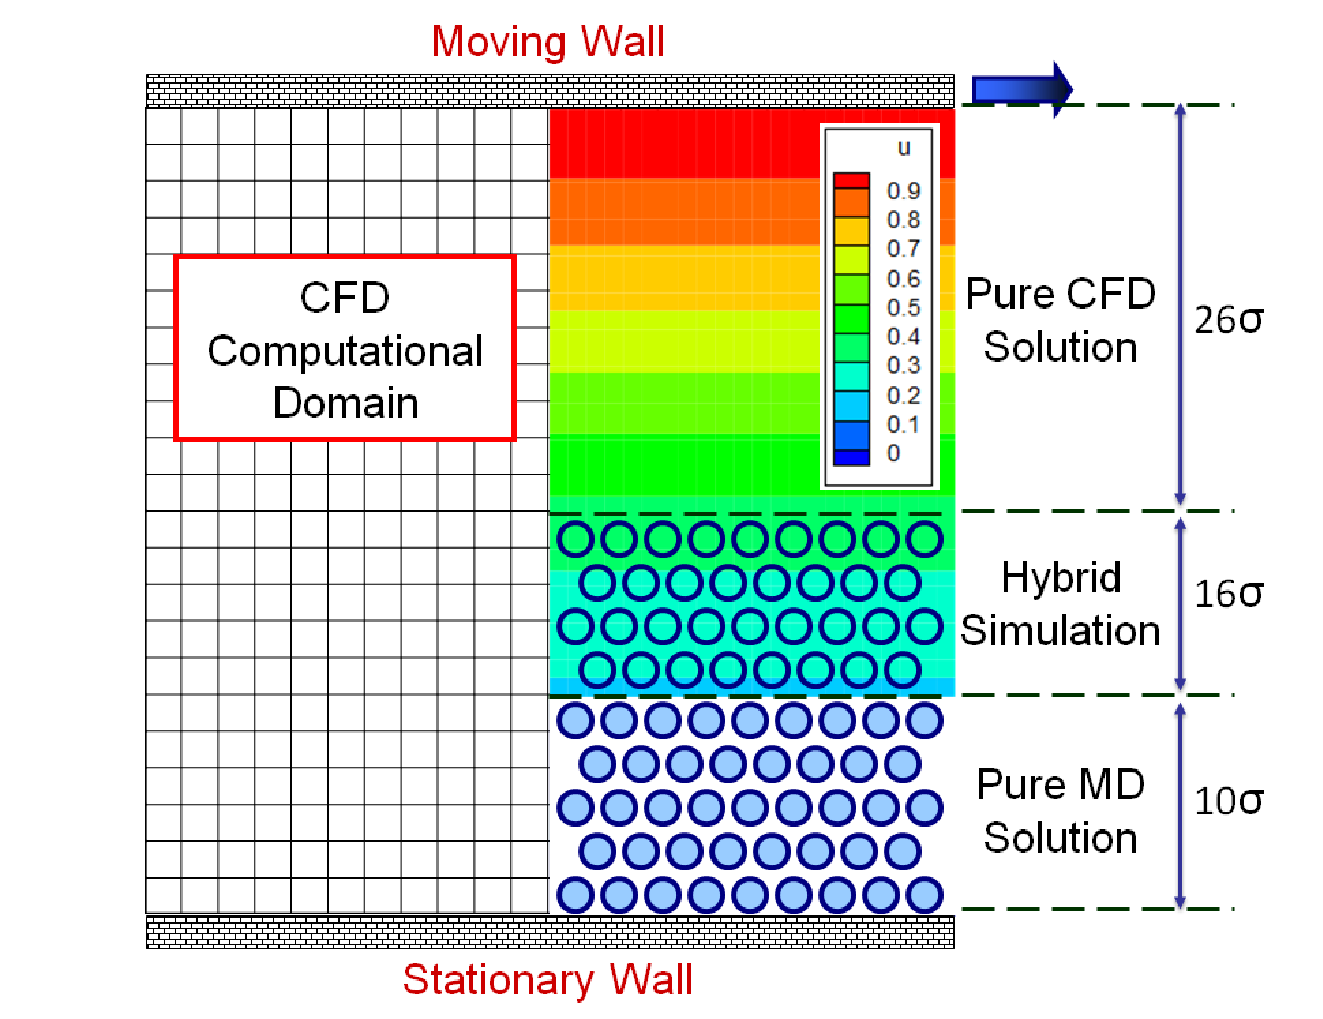
\includegraphics[width=0.8\linewidth]{Couette_Val_Domain.pdf}
\vskip-0.2cm
\caption{\small Computational Domain of Couette Flow Simulation; The height of the fluid domain is 52$\sigma$ ($\approx$177$\AA$). CFD mesh size is 71$\times$27 and CFD cells at the pure MD region are treated as holes. MD domain size is about 140$\sigma$ in the X-direction and around 26$\sigma$ in the Y-direction, including the bottom wall. Periodic boundary condition is applied on the principal flow direction.}
\label{Couette_Val_Domain}
\end{figure}


%The same measurement has been conducted on 10$^{-7}$ meter domain. Table~\ref{table:MD_Vel0_L} shows that the strength of statistical error with different layer height and sampling duration. The length of the system domain is fixed to be 140 $\sigma$ for the direct comparison with the last experiment in Table~\ref{table:MD_Vel0}.
%The strength of the noise in this large system is globally milder than the result in small system in Table~\ref{table:MD_Vel0}. Furthermore, the quantitative comparison between this result and the above solution at the same domain length (third table in Table~\ref{table:MD_Vel0}) proves that the noise in large system is always smaller at the same conditions, e.g., measured noise at 4$\sigma$-40$\tau$ condition in large system is smaller than the noise at 6.4$\sigma$-64$\tau$ condition in small system. However, more delicate selection of coupling conditions is highly required as system size increases, because the hydrodynamic characteristic time scale (or time for steadiness) is proportional to the square of system height.~\cite{Hadjicon3} In our simulation, we set the CFD cell size (the same as the height of individual layer) as 16$\sigma$, sampling duration as 100$\tau$. This force us to place the hybrid domain 80 $\sigma$ above the bottom wall, where the statistical error is about 2.5 percent of the steady-state velocity in Couette flow.


%% Table formats; h,t,b,p - here,top,bottom,page of floats
%%\begin{table}[t]
%\begin{table}
% \caption{\small Statistical Error Measurement on Large System Domain; System is bound by upper and lower walls and has the domain of 140 $\times$ 520 ${\sigma}^2$. Data from 1000 $\tau$ to 3560 $\tau$ are accumulated and post-processed to figure out the variation of statistical noise at different layer size and sampling duration conditions. The unit is 1/1000 of non-dimensional MD velocity (1$\sigma / \tau$).}
% \label{table:MD_Vel0_L}
% \centering
%  \resizebox{0.8\linewidth}{!} {
%  \begin{tabular}{c || c c c c c c c}
%\hline
%	&	10 $\tau$	&	20 $\tau$	&	40 $\tau$	&	80 $\tau$	&	160 $\tau$	&	320 $\tau$	&	640 $\tau$	\\
%\hline
%1 $\sigma$	&	11.711 	&	9.739 	&	8.287 	&	6.607 	&	5.284 	&	4.201 	 &	2.698 	\\
%2 $\sigma$	&	10.375 	&	9.116 	&	7.760 	&	6.271 	&	5.112 	&	3.802 	 &	2.760 	\\
%4 $\sigma$	&	8.362 	&	7.804 	&	6.870 	&	5.983 	&	5.236 	&	3.760 	 &	2.952 	\\
%8 $\sigma$	&	6.046 	&	5.763 	&	5.346 	&	4.826 	&	4.429 	&	3.674 	 &	3.056 	\\
%16 $\sigma$	&	4.424 	&	4.348 	&	4.272 	&	4.030 	&	3.941 	&	 3.629 	 &	2.850 	\\
%32 $\sigma$	&	2.706 	&	2.683 	&	2.639 	&	2.603 	&	2.481 	&	 2.277 	 &	1.981 	\\
%64 $\sigma$	&	1.757 	&	1.735 	&	1.714 	&	1.697 	&	1.642 	&	 1.535 	 &	1.505 	\\
%%128 $\sigma$	&	0.975 	&	0.970 	&	0.964 	&	0.958 	&	0.934 	&	 0.925 	&	0.925 	\\
%\hline
%%\hline
%%L=140,Vtot	&	10 $\tau$	&	20 $\tau$	&	40 $\tau$	&	80 $\tau$	&	 160 $\tau$	&	320 $\tau$	&	640 $\tau$	\\
%%\hline
%%1 $\sigma$	&	11.833 	&	9.914 	&	8.642 	&	7.527 	&	6.130 	&	 5.746 	 &	5.322 	\\
%%2 $\sigma$	&	10.585 	&	9.280 	&	8.611 	&	7.570 	&	6.630 	&	 6.103 	 &	5.694 	\\
%%4 $\sigma$	&	9.048 	&	8.498 	&	8.027 	&	7.422 	&	6.489 	&	 6.256 	 &	6.076 	\\
%%8 $\sigma$	&	7.391 	&	7.185 	&	6.957 	&	6.762 	&	6.392 	&	 6.248 	 &	6.189 	\\
%%16 $\sigma$	&	6.764 	&	6.719 	&	6.633 	&	6.588 	&	6.444 	&	 6.428 	&	6.428 	\\
%%32 $\sigma$	&	5.656 	&	5.648 	&	5.636 	&	5.631 	&	5.626 	&	 5.627 	&	5.627 	\\
%%64 $\sigma$	&	3.721 	&	3.717 	&	3.717 	&	3.717 	&	3.702 	&	 3.684 	&	3.684 	\\
%%%128 $\sigma$	&	1.802 	&	1.795 	&	1.790 	&	1.779 	&	1.761 	&	 1.743 	&	1.678 	\\
%%\hline
%\end{tabular} }
%\vspace{-1em}
%\end{table}



\subsection{A Sudden-start Couette Flow}
\label{sec:accuracy_couette}

%The first problem is the Couette flow simulation, which have been in wide use for the validation of a hybrid CFD-MD solver.~\cite{Nie},\cite{Yen} We start from the validation case, which has 52$\sigma$ distance between two parallel plates and upper wall velocity is ${\sigma}/{\tau}$. We assume liquid argon particles are filled in the domain and both walls have artificial properties which is the same as those of liquid argon. Characteristic length of liquid argon is ${\sigma}=3.405{\times}10^{-10}$ and time scale is $\tau=2.2{\times}10^{-12}$. Density is $0.81m{\sigma}^{-3}$, which means 0.81 atoms are included in the characteristic volume.

%Table \ref{table:MD_Vel0} shows the averaged velocity on different layer size and sampling duration. Experiments were conducted with different system width changing from 35 $\sigma$ to 70 and 140 $\sigma$. From the individual test, we can find that increasing sampling duration or height of averaged layer does not linearly decrease the statistical error. At the first test, increasing the height of averaged layer from 0.1 $\sigma$ to 6.4 $\sigma$ reduces the statistical error by 4 times when sampling duration is 1 $\tau$ and this ratio even gets worse as sampling duration increases. The same situation also happens on sampling duration. Next, by comparing the first and third experiments, we find that the statistical error in general becomes half when the system size is 4 times bigger. This does not support the conclusion of statistical error analyses~\cite{Hadjicon2},\cite{Time_Mechanism} where the strength of error is inversely proportional to the system size. We assume that the upper and lower walls hinder the noise from being damped out. Nevertheless, increasing the system domain is more effective than numerically increasing the size of averaged layer in reducing the statistical error. Lastly, though not included in this table, we also conducted numbers of experiments by changing time step in MD simulation, $\Delta t_{MD}$. We could not find much difference in the strength of statistical noise with different time step and this concludes us that this fluctuation and its scale is physically natural phenomenon. So, time step for MD simulation is fixed as $\Delta t_{MD}=5 \times 10^3 \tau$ on all simulations.

A sudden-start Couette flow is simulated to verify the accuracy of the current framework with multiple sampling approach for the moderate-speed flow simulation. This application has been in wide use for the validation of a hybrid CFD-MD solver.~\cite{Nie,Yen} The flow is initially set stationary and the upper wall starts moving by a constant velocity (1 $\sigma$/$\tau$). This physical boundary condition of the continuum domain governs the evolution of the whole flow field. Figure~\ref{Flat_Plate_Sol} presents a sudden-start Couette flow profile by CFD, MD and hybrid simulations.
% in 10$^{-8}$ meter system.
Pure CFD produces identically the same result as analytic solution and MD simulations also describes the same flow physics though the slight fluctuation of the solution is observed. This verifies the accuracy of the individual solver. The hybrid solution also shows the slight deviation from the analytic solution, which is the fluctuation of the sampled MD solution. Nevertheless, the hybrid simulation succeeds in demonstrating the same flow physics as the analytic solution. This variation can even be diminished if the solution is visualized over a longer temporal range, which is observed in many articles.
This proves that the current hybrid framework accurately analyzes the steady flow profile in nano-scaled systems.


%\begin{figure}[ht]
\begin{figure}
\centering
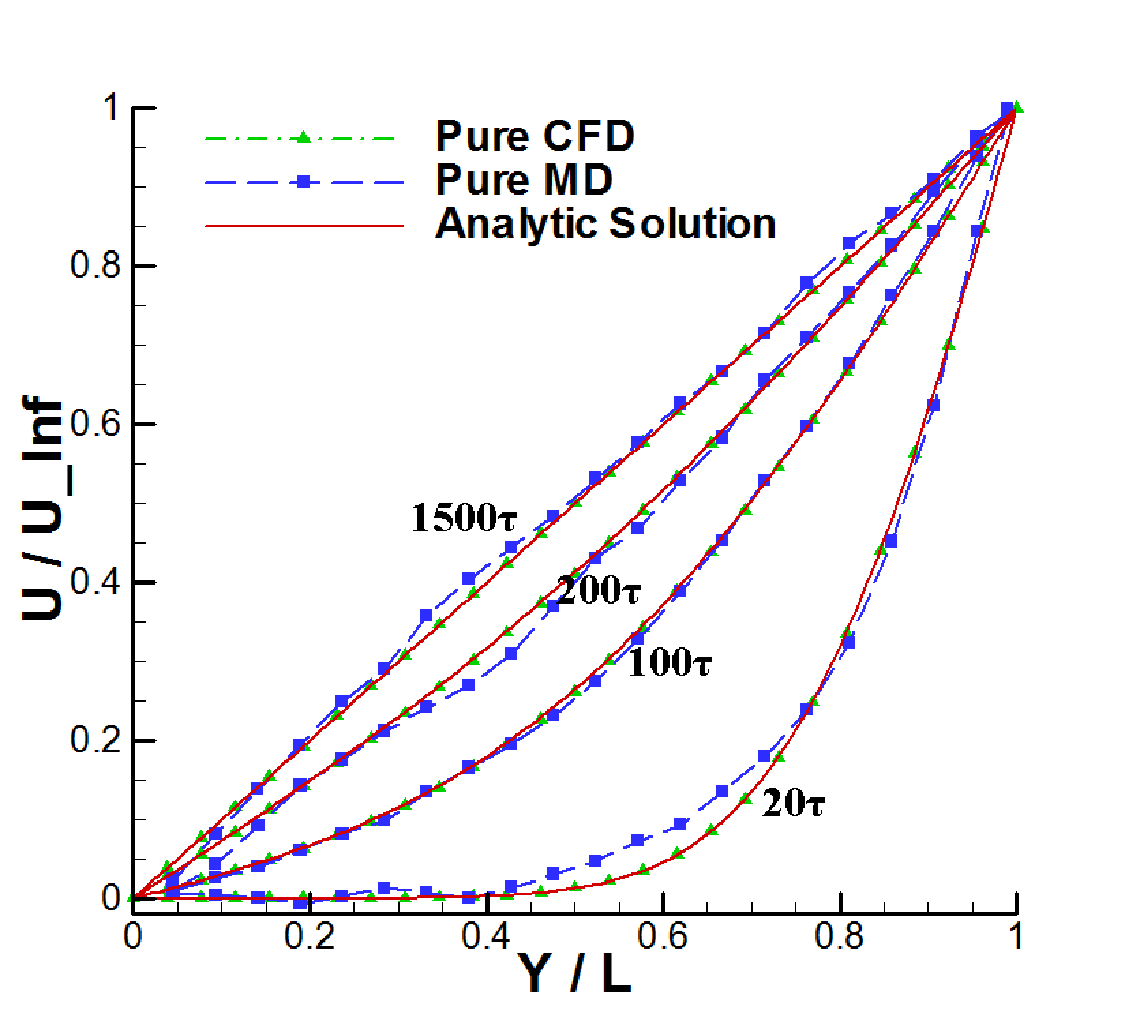
\includegraphics[width=0.6\linewidth]{Flat_Plate_Sol1.pdf}
\hskip 1cm
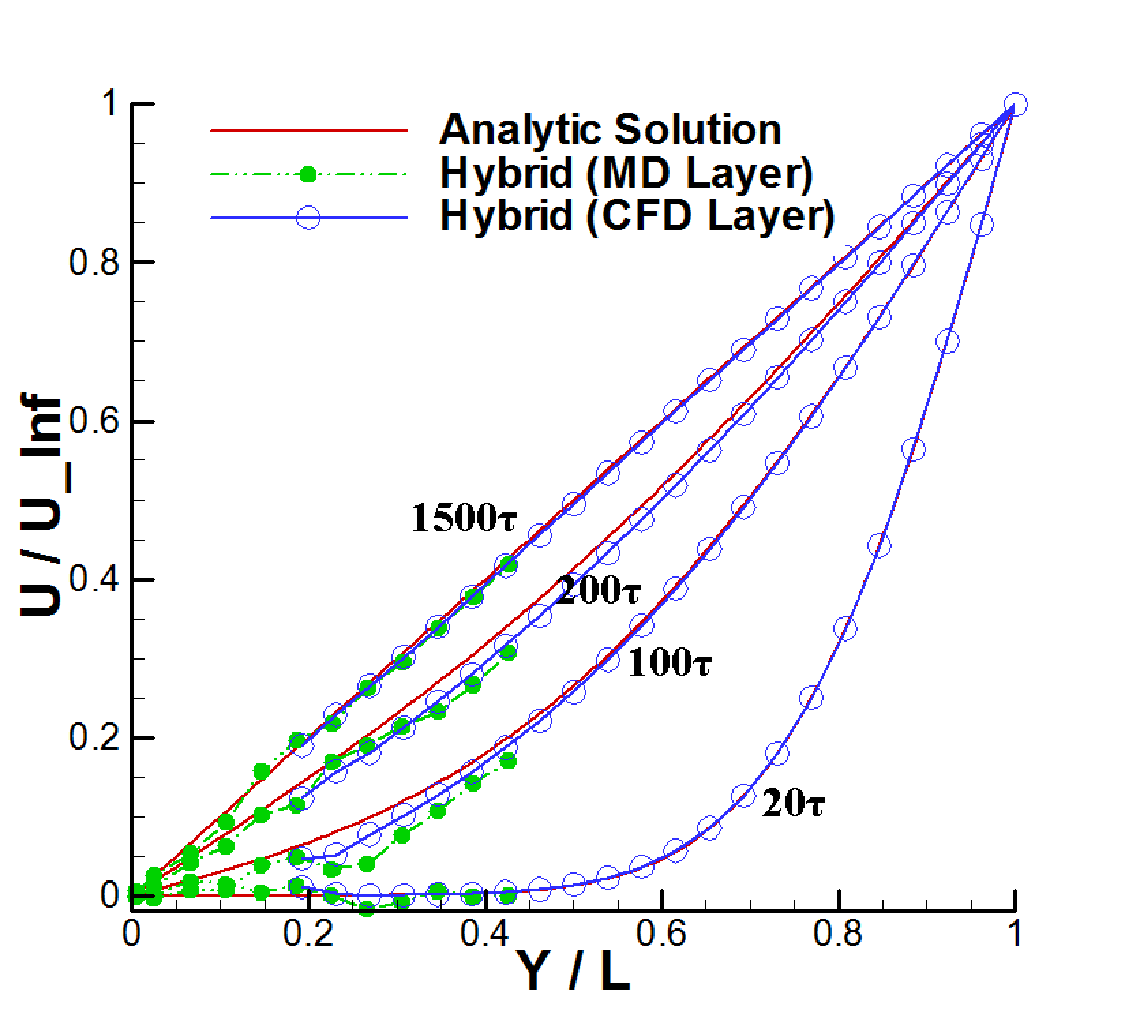
\includegraphics[width=0.6\linewidth]{Flat_Plate_Sol2.pdf}
\vskip-0.2cm
\caption{\small Unsteady Couette Flow Profile; The evolution of velocity field along the vertical direction is presented. CFD solution is the instantaneous profile at specified time and MD solution is spatially averaged over 2 $\sigma$ in height and temporally averaged for 1 sampling durations (=10$\tau$). (Left) Pure CFD solution is exactly the same as analytic solution. MD solution shows the same flow pattern as analytic solution, though some fluctuation is observed. This verifies that CFD and MD represents the same flow physics. (Right) The steady result by hybrid approach produces the same numerical result as analytic solution, though the slight time-lagging in the hybrid boundary is observed during the evolution.}
\label{Flat_Plate_Sol}
\end{figure}


%We now apply our framework on solving the flow field with 10$^{-7}$ meter scale. In this simulation, all conditions are identical to above simulation, except the height of the system becomes 10 times bigger (520$\sigma$) in height. As has been argued by Yen {\it{et al.}}~\cite{Yen}, the influence of thermal fluctuation becomes quite stronger in the simulation of the low shear rate flow, which can cause the unfavorable convergence characteristics. We believe that this numerical analysis at low shear rate condition evaluates the accuracy of our framework.

%Figure~\ref{Flat_Plate_Sol_L} shows the velocity profile of the Couette flow by a hybrid simulation compared with the analytic solution. Hybrid zone is composed of two layers for MDtoCFD boundary, one for buffer, two for CFDtoMD solution, another one buffer and one external force layer, starting from the bottom. The result by hybrid simulation is in good agreement with the analytic solution throughout the time domain, which evaluates the accuracy of our numerical implementation. Plotted results are instantaneous CFD solutions (MD solutions averaged over one sampling duration) without the filtering over a long physical time: this explains that the slight variation in steady-state solution is caused by the local fluctuation at that instance.


%%\begin{figure}[ht]
%\begin{figure}
%\centering
%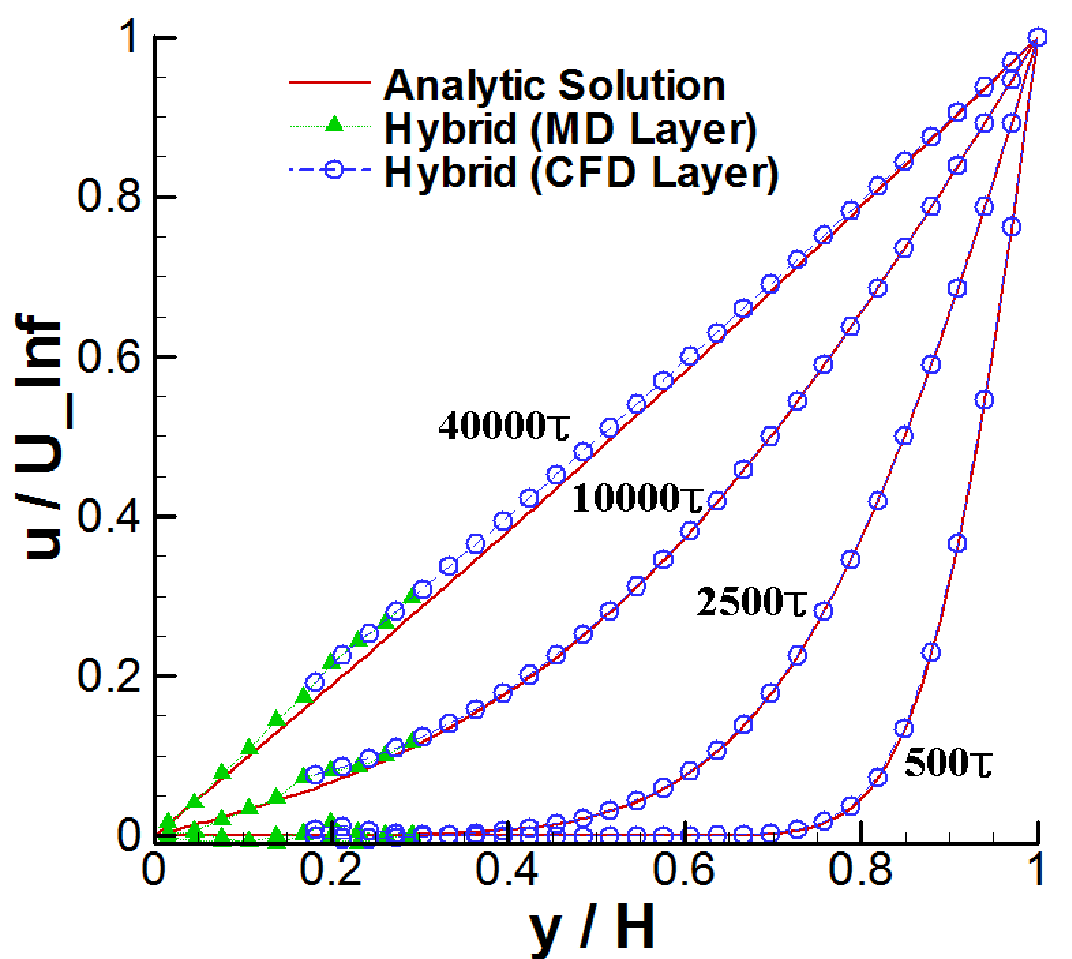
\includegraphics[width=0.6\linewidth]{Couette_Large.pdf}
%\vskip-0.2cm
%\caption{\small Couette Flow Profile in O(100) Nanometer Domain; The variation of non-dimensionalized horizontal velocity along the vertical direction is plotted . CFD solutions at each specified time and MD solutions averaged over 100 $\tau$ are compared with the analytic solution. Overall solutions match quite well with analytic solution.}
%\label{Flat_Plate_Sol_L}
%\end{figure}


The flow condition in above experiment is rather unrealistic, which motivates us to apply the hybrid scheme to the analysis of moderate velocity flow. As has been expressed in Sec.~\ref{sec:numerical_lowspeed}, hybrid simulation of the low-speed flow field is mathematically possible but technically bound by the computing capacity, since the computational domain becomes $u^2$ times bigger in solving $1/u$ velocity field. We instead run $u^2$ independent simulations with the initial system size and different random number seeds in LAMMPS package. %A BigJob framework helps in scheduling multiple job execution and data management.


The Couette flow profile with different numbers of samples are presented in Fig.~\ref{multiple_couette}. All configurations and parameters are identical to the above validation problem, except the upper plate velocity of 0.25 $\sigma/\tau$. Changing the velocity to 1/4 implies that averaging 16 samples are required to get the acceptable numerical solution. The result supports the above supposition. The solution becomes very accurate when 16 individual runs are sampled. The reduction of statistical noise by multiple samplings is clearly verified by the graph in Fig.~\ref{multiple_couette_temporal}. The noise is roughly seen to reduce by half with 4 times more samples and the solution of sampling 16 runs shows about 5 $\%$ of the noise compared to the analytic solution profile.


%\begin{figure}[ht]
\begin{figure}
\centering
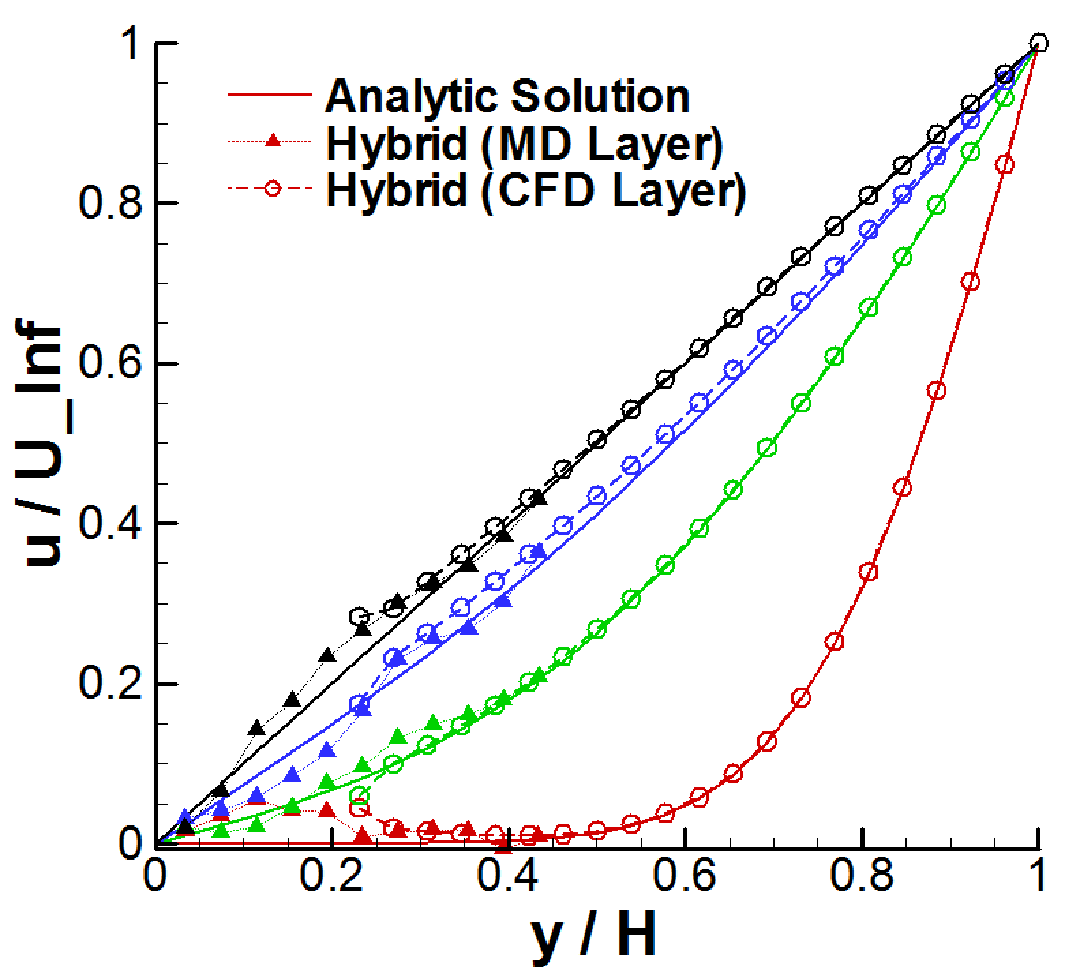
\includegraphics[width=0.6\linewidth]{Couette_025_Samp4.pdf}
\hskip 1cm
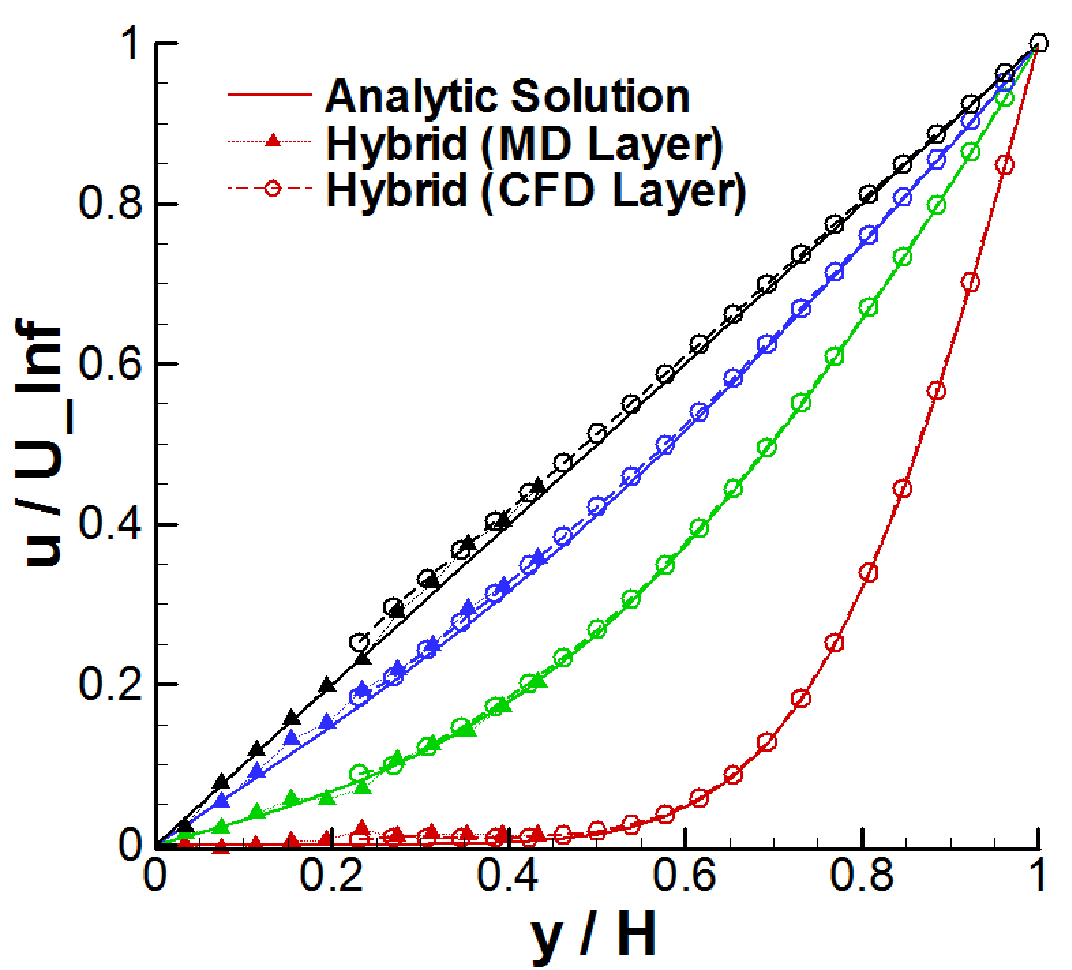
\includegraphics[width=0.6\linewidth]{Couette_025_Samp16.pdf}
\vskip-0.2cm
\caption{\small Couette Flow Profile with the Upper Plate Velocity of 0.25 $\sigma/\tau$; The noisy solution when 4 individual simulations are averaged (left) is resolved by sampling 16 independent runs (right). Red lines denote the solution at 20 $\tau$; Green, blue and black lines are solutions at 100, 200 and 1500 $\tau$, respectively.}
\label{multiple_couette}
\end{figure}

\begin{figure}
\centering
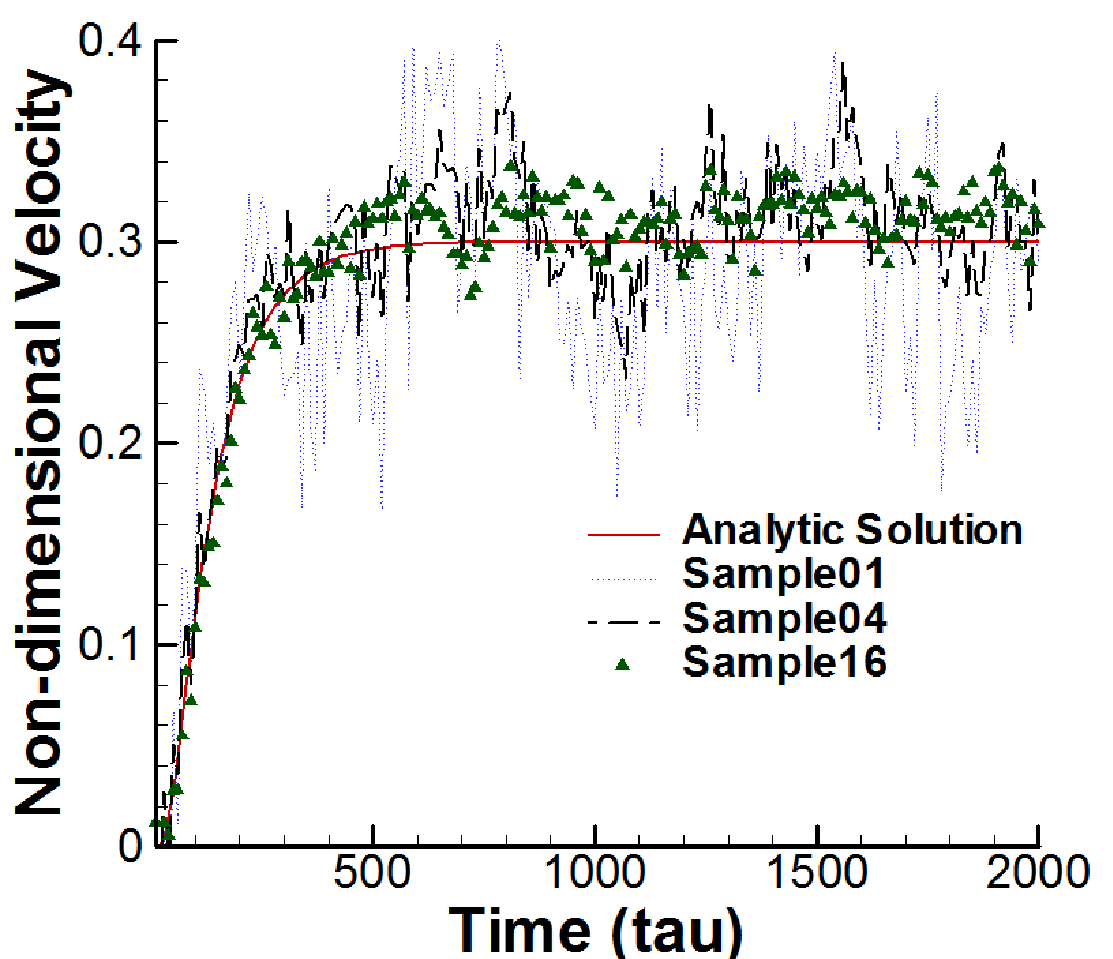
\includegraphics[width=0.6\linewidth]{Couette_025_Temporal_Multiset.pdf}
\vskip-0.2cm
\caption{\small Variation of Continuum Velocity at the Position of 0.3 Height from the Bottom Wall (Middle of the Overlapping Region); Velocity changes at various sampling runs are compared with the analytic solution. In case 16 simulations are averaged, the noise is about 5 $\%$ compared to the analytic solution.}
\label{multiple_couette_temporal}
\end{figure}


The solution by multiple sampling is compared with the solution in increased system domain. Figure~\ref{increase_system} shows the Couette flow profile with 16 times bigger system size in horizontal direction and the comparison of velocity variation in the middle of the overlapping region. From the result, both ways (multiple sampling and increasing system size) produce acceptable numerical solutions compared to the analytic solution. Interestingly, the scale of the noise compared to the analytic solution is very similar in both ways, which verifies that multiple sampling approach can replace the increase of system size to reduce the statistical error.

%\begin{figure}[ht]
\begin{figure}
\centering
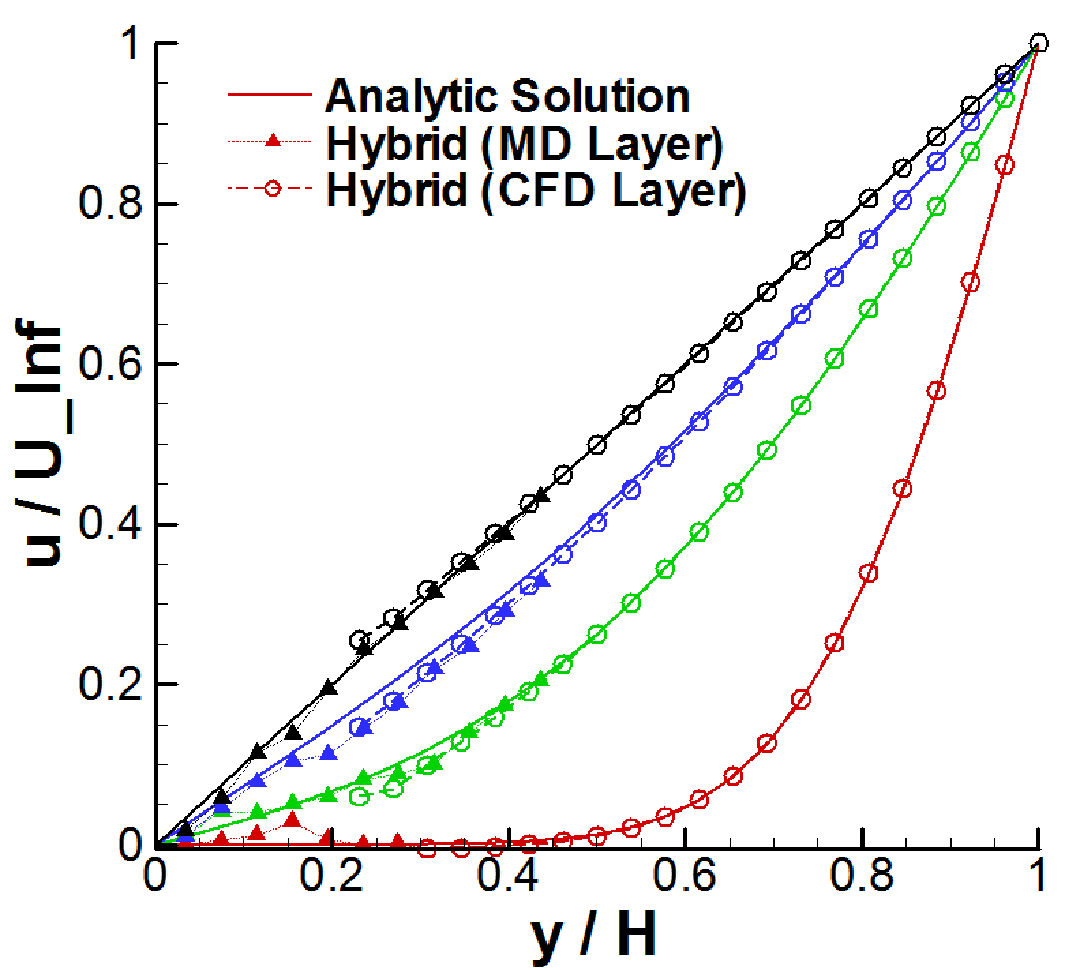
\includegraphics[width=0.6\linewidth]{Couette_025_Scale16.pdf}
\hskip 1cm
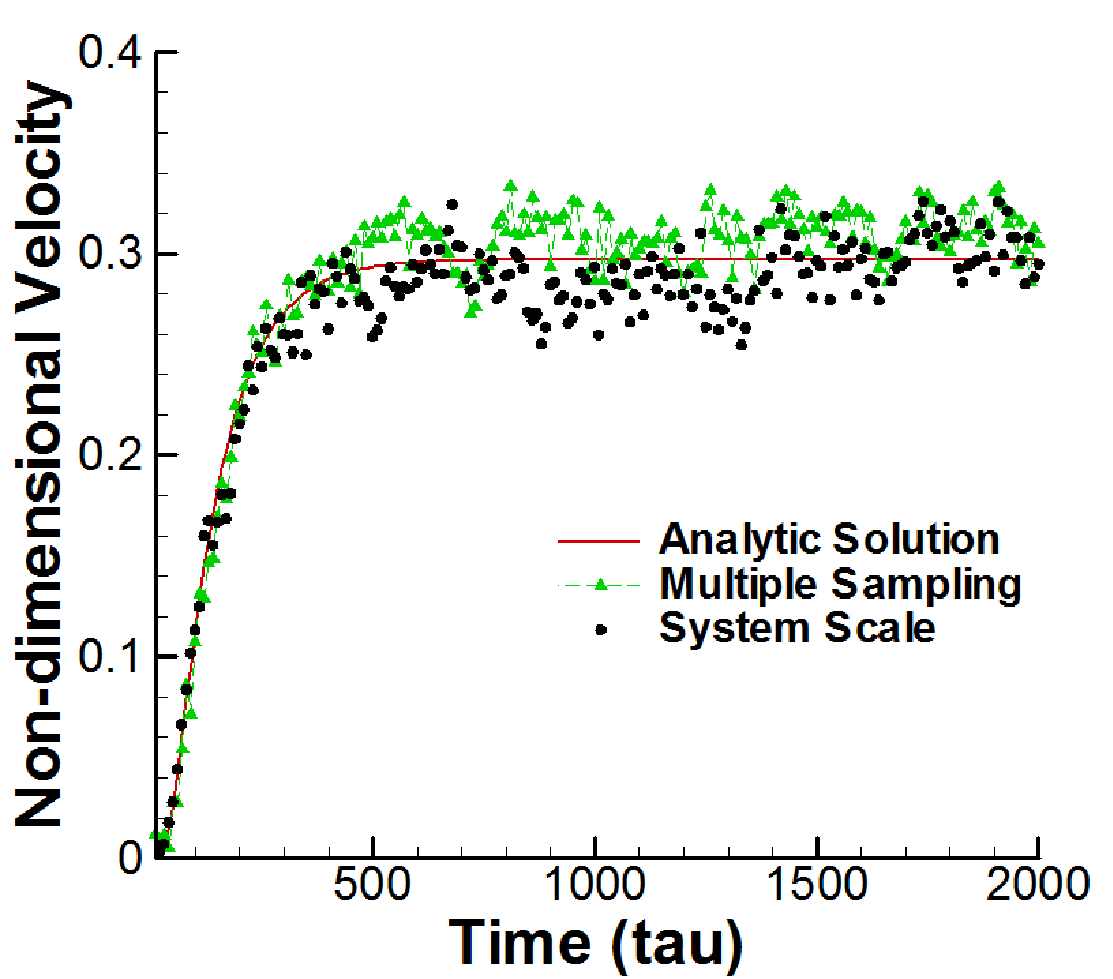
\includegraphics[width=0.6\linewidth]{Couette_025_Temporal_Multiset_VS_Scaleup.pdf}
\vskip-0.2cm
\caption{\small (Left) Couette Flow Profile in Increased System Size; Accurate flow profile can be obtained by increasing the system size 16 times larger when the velocity is reduced to 1/4. Red lines denote the solution at 20 $\tau$; Green, blue and black lines are solutions at 100, 200 and 1500 $\tau$, respectively. (Right) Variation of the Velocity in the Middle of Overlapping Region; Solutions by multiple sampling and increasing the system contain the similar strength of the noise in the solution, which is around 5 $\%$ of analytic velocity profile. This implies that multiple sampling approach can replace the increase of system size for solving moderate velocity flow.}
\label{increase_system}
\end{figure}


Collectively, results by multiple samples show the same order of accuracy compared to the increase of the system size. Especially in cases the physical system is large, multiple sampling is more effective than directly increasing the system size, because excessively large-scaled jobs (in view of wall-time limit or number of resources requested) are very hard to get allocated. In addition, the labor of manually submitting multiple independent runs and managing data sets can be relieved by adopting a BigJob framework.


\subsection{A Physically Unsteady Flow Field: Oscillating Boundary Problem}
\label{sec:accuracy_oscillation}

The accuracy of designed temporal coupling scheme is verified by solving an unsteady oscillating boundary problem. In Couette flow simulation, which converges to a steady-state flow profile, the minor inaccuracy during the flow evolution can be eventually recovered. On the other hand, the inaccurate solution at an one instance harms the flow field afterwards in this physically unsteady problem. Therefore, the accuracy of temporal coupling scheme becomes more important. Also, velocity in the hybrid region becomes far slower than the Couette flow profile, so that the influence of noise from MD side is concerned to be more critical in the current flow simulation. The computational domain and coupling conditions are the same as the above Couette flow simulation. In this case, the upper wall boundary condition changes from the fixed velocity to oscillatory wall, which is $u_{wall}(t)=({\sigma}/{\tau}){\times}sin(2{\pi}t/T)$. Period $T$ is set to be 200$\tau$.
% in 10$^{-8}$ meter system.


Figure~\ref{Stokes_Sol} shows the oscillatory velocity profile by pure CFD and hybrid simulations. From the left figure, velocity profiles at each time instance are roughly the same between the pure CFD and hybrid simulations in magnitude. This provides that the hybrid simulation approach is also applicable to time-varying flow simulations. Meanwhile, the temporal variation of the horizontal velocity in the middle of hybrid region expresses that the noise in hybrid solution is not negligible considering the ratio between continuum and hybrid velocities. We claim that this noisy solution is caused by the combination of sampling error and inaccurate temporal coupling scheme. To clearly examine the effect of temporal coupling scheme, we sampled multiple independent experiments and compared solutions by different temporal coupling schemes.

%In detail, fluctuation in MD domain is not so strong in hybrid region. Though minor time-lagging profile is seen from MD solution, this does not change the global flow profile dominantly because the driving force in this simulation is the oscillating velocity from CFD domain.

%\begin{figure}[ht]
\begin{figure}
\centering
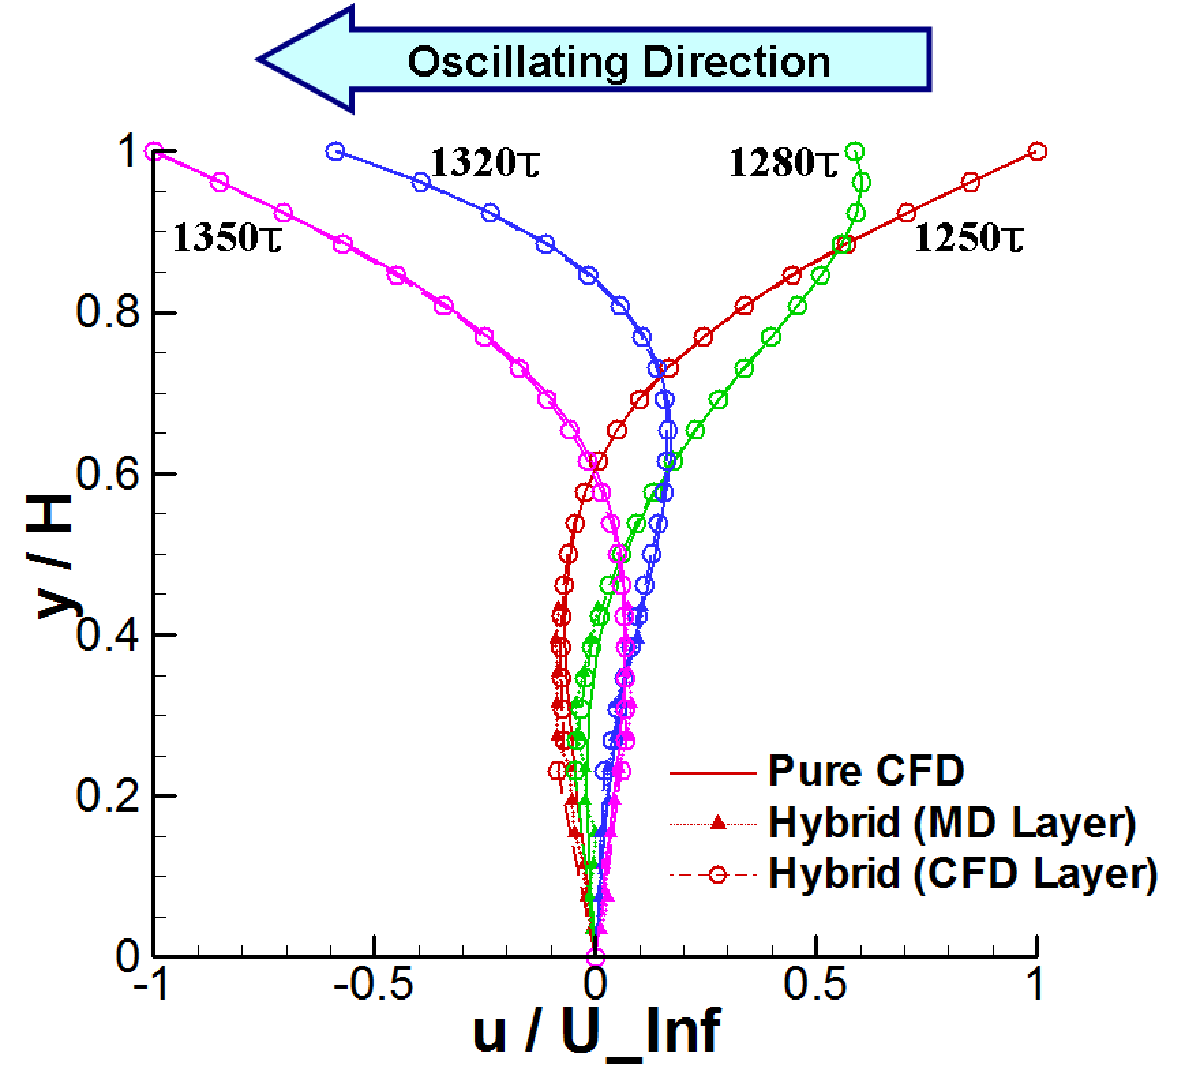
\includegraphics[width=0.6\linewidth]{Stokes_Sol_Profile.pdf}
\hskip 1cm
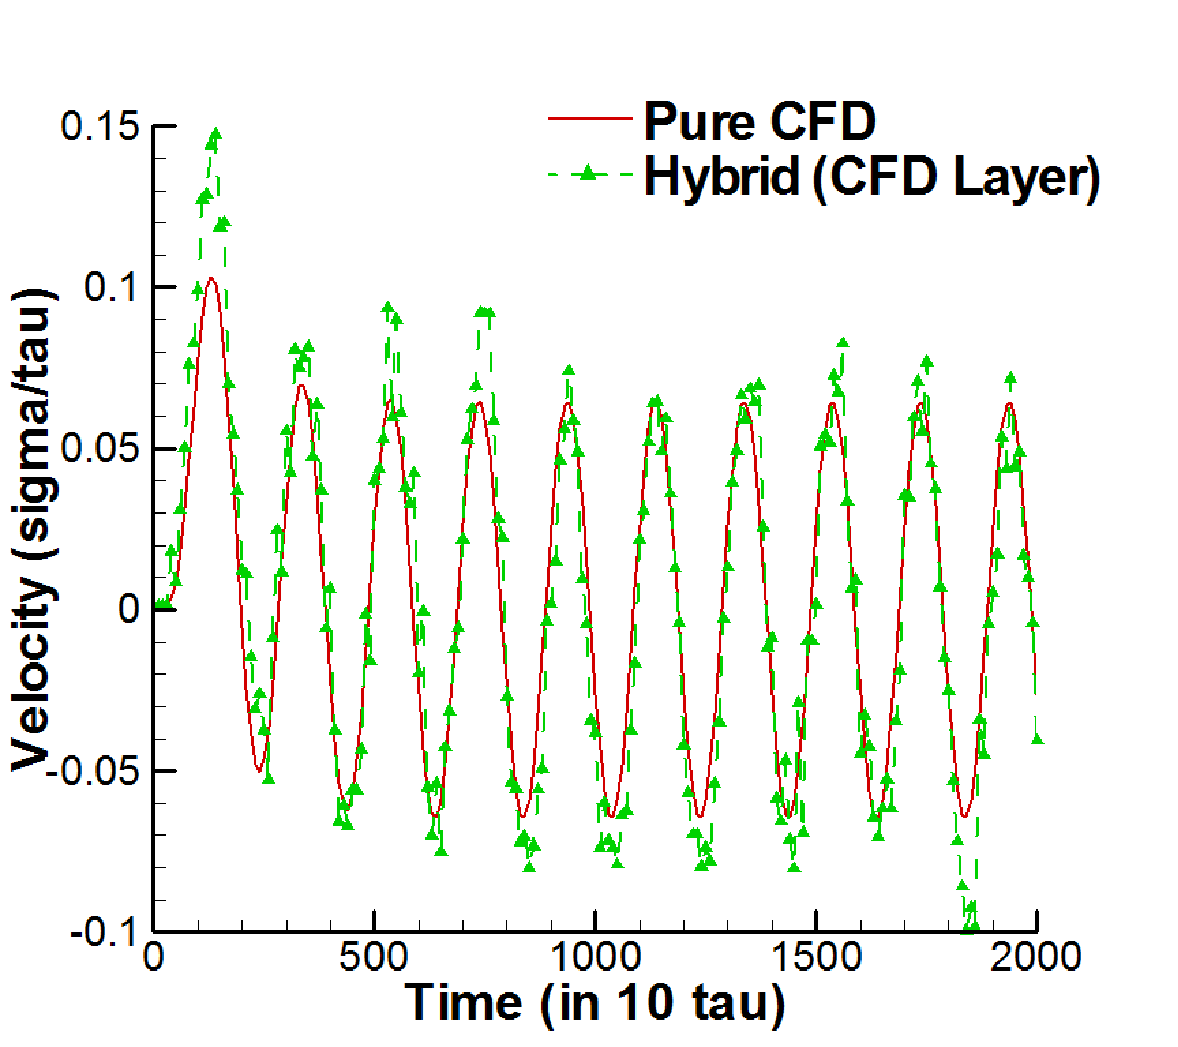
\includegraphics[width=0.6\linewidth]{Stokes_Temporal_Profile.pdf}
\vskip-0.2cm
\caption{\small Unsteady Flow Profile of Stokes Boundary Layer Problem; (Left) Velocity profiles by pure CFD and hybrid simulations at specified time instances. Difference between hybrid and pure CFD solutions in hybrid region shrinks in the continuum domain. Noise from the MD simulation does not affect the global velocity profile a lot, because the driving force in this simulation is the oscillating velocity from CFD domain. (Right) Temporal variation of the velocity in the middle of hybrid layer. History of the velocity field reveals that the hybrid solution contains much noise in this experiment.}
\label{Stokes_Sol}
\end{figure}


Comparing temporal evolutions of the velocity field by different coupling schemes in Fig.~\ref{Temporal1}, the clear difference is the resolution of the overshoot/undershoot phenomena by the prediction-correction approach. Sufficient numbers of independent experiments are sampled to reduce the statistical error and prediction time scale of 2.5 sampling intervals is chosen on prediction-correction approach to impose the interpolated boundary conditions on both domains. On conventional model, the maximal error is seen at peak points. This is a natural characteristics of the linear extrapolation that it fails to predict the correct values around the strong variation. This inaccuracy is resolved by using a prediction-correction approach and applying interpolated boundary condition from predicted flow properties. However, another numerical inaccuracy of time-lagging pattern in conventional model is also seen in the prediction-correction model. This necessitates the implementation of higher-order interpolation schemes.


%\begin{figure}[ht]
\begin{figure}
\centering
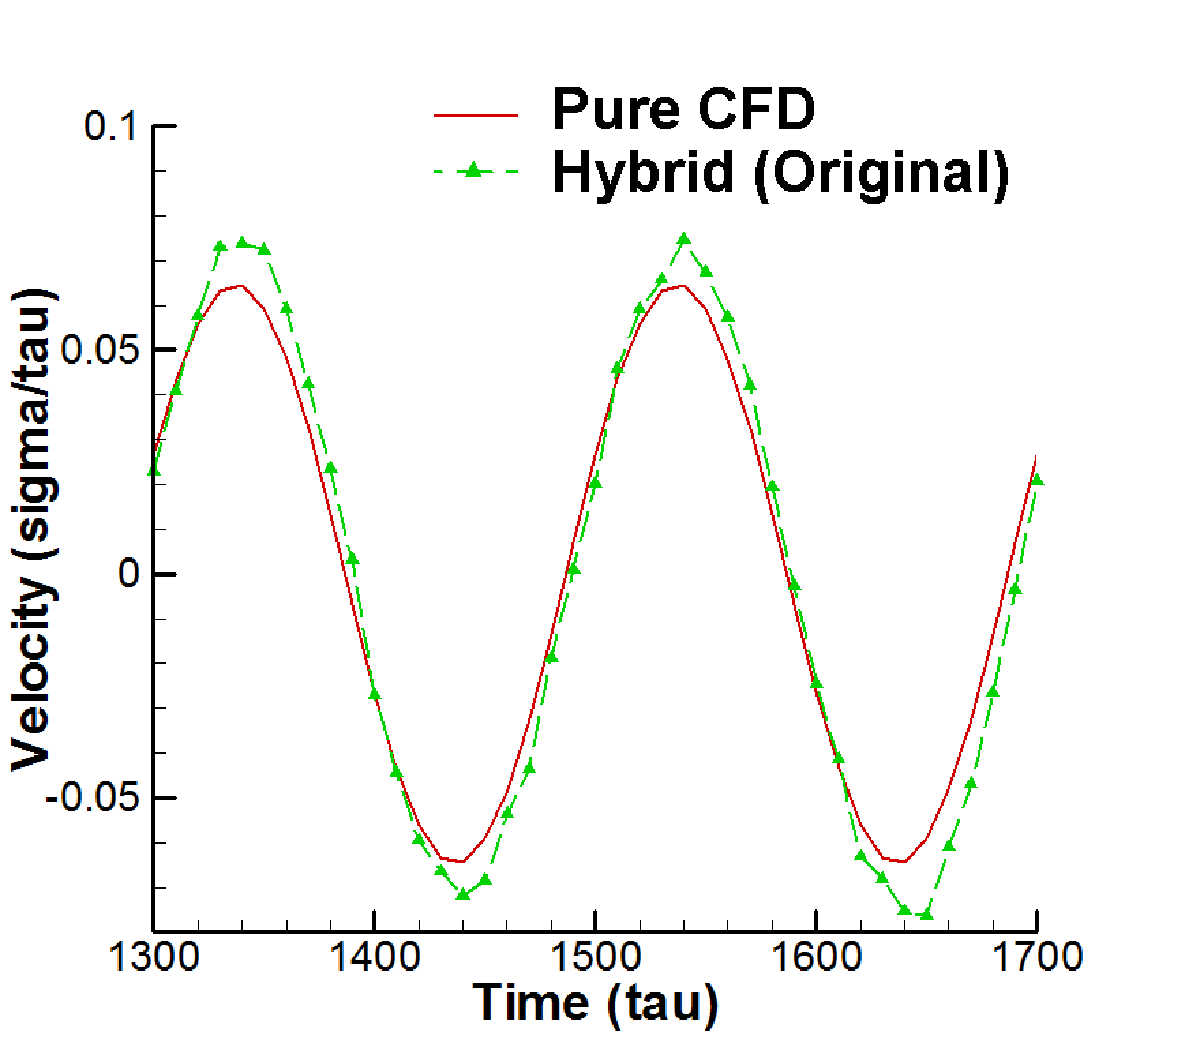
\includegraphics[width=0.6\linewidth]{Stokes_Org_Multi.pdf}
\hskip 1cm
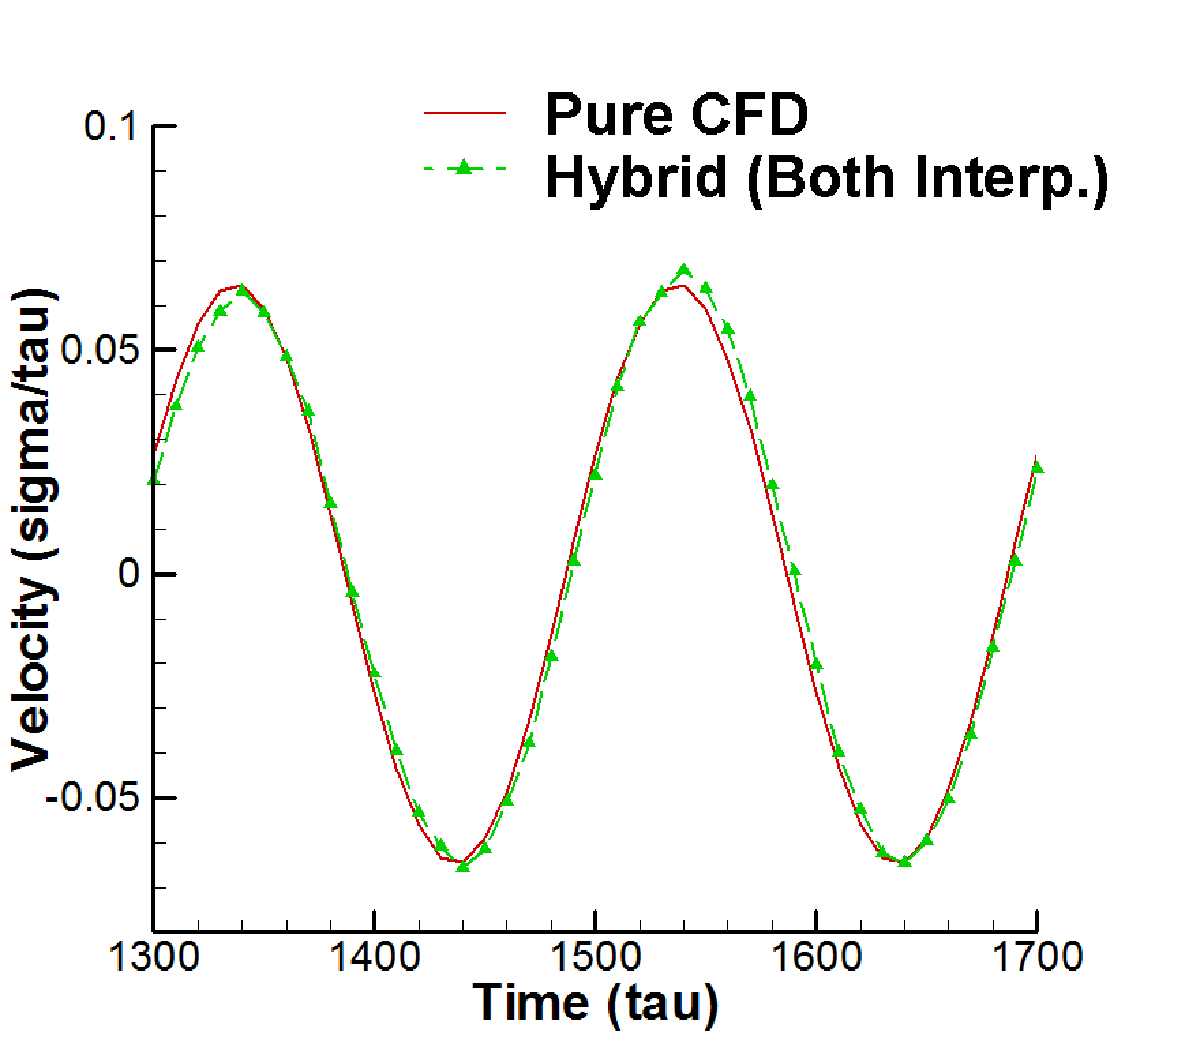
\includegraphics[width=0.6\linewidth]{Stokes_Both_Multi.pdf}
\vskip-0.2cm
\caption{\small Temporal Variation of the Velocity in the Middle of Hybrid Layer; (Left) With conventional model, large overshoot/undershoot phenomena are observed on the peak points: the statistical noise around 0.01 $\sigma/\tau$ is nearly 20 $\%$ of continuum velocity. The time-lagging effect is also captured. (Right) Overshoot/undershoot phenomena in the conventional approach is almost resolved by applying the prediction-correction approach. The interpolated hybrid boundary conditions are imposed on CFD and MD domains.}
\label{Temporal1}
\end{figure}


Plots in Fig.~\ref{Temporal2} quantifies the scale of inaccuracy according to the hybrid boundary condition imposition. In the conventional model, the velocity difference ranges from -0.017 to 0.015 $\sigma/\tau$. The magnitude of this error reduces as we apply the prediction-correction approach and increase the prediction time scale from 0.5 (corrected extrapolation) to 1.5 (MD interpolation) and 2.5 (both interpolation) sampling intervals. The clear difference between the conventional extrapolation model and corrected extrapolation in prediction-correction approach demonstrates that the extrapolation from two ''previous'' properties contains a lot more error compared to extrapolating from the current value. The similar variation between extrapolation and MD interpolation in prediction-correction approach emphasizes that the accuracy of boundary condition in CFD domain is as important as the boundary condition in MD domain. Lastly, the solution error form the conventional model is reduced by half with the imposition of interpolated boundary conditions on both domains.


%\begin{figure}[ht]
\begin{figure}
\centering
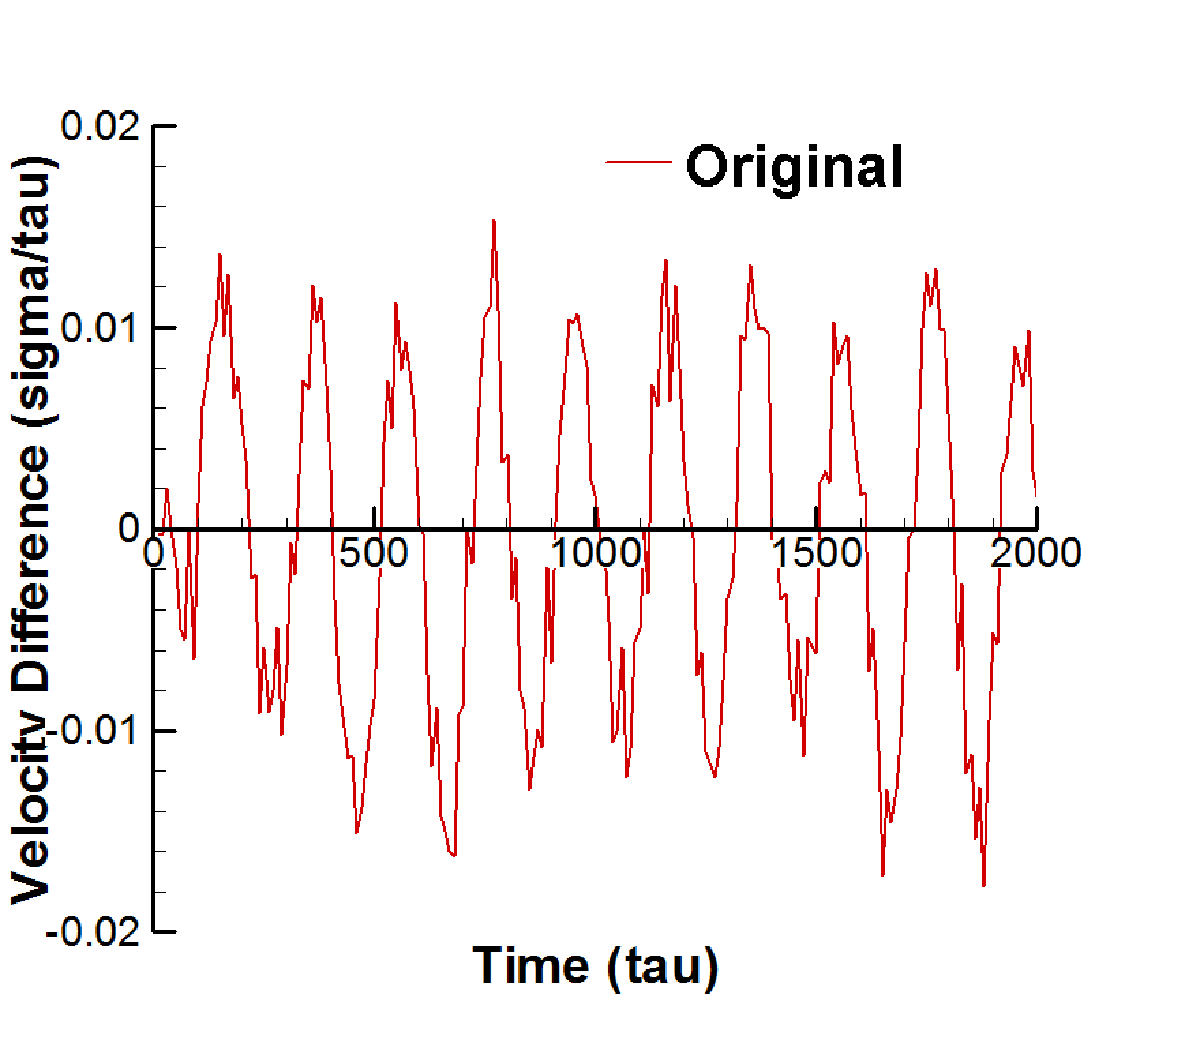
\includegraphics[width=0.45\linewidth]{Stokes_Org_Diff.pdf}
\hskip 1cm
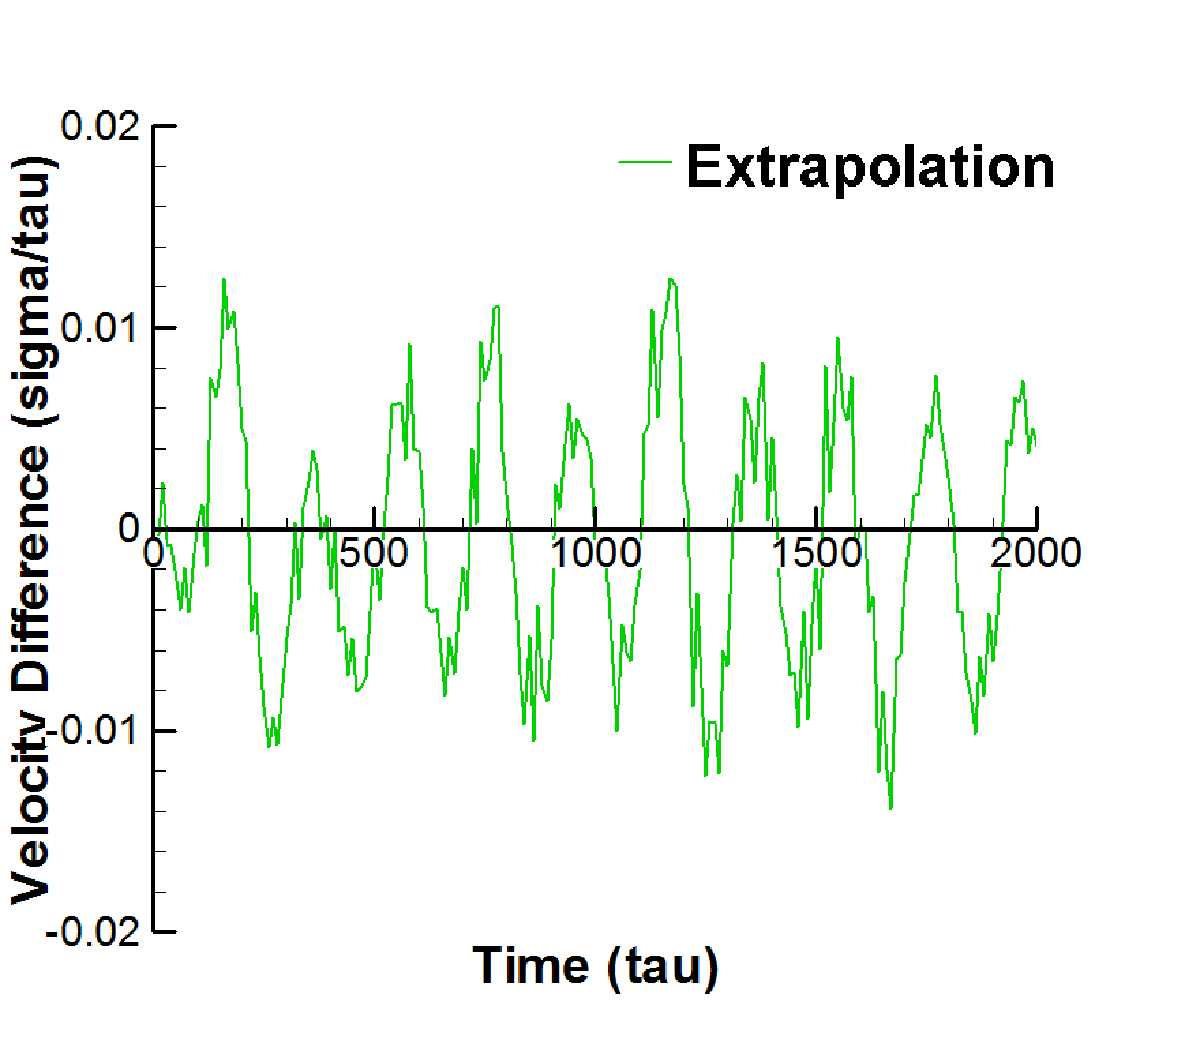
\includegraphics[width=0.45\linewidth]{Stokes_Exp_Diff.pdf}
\vskip-0.2cm
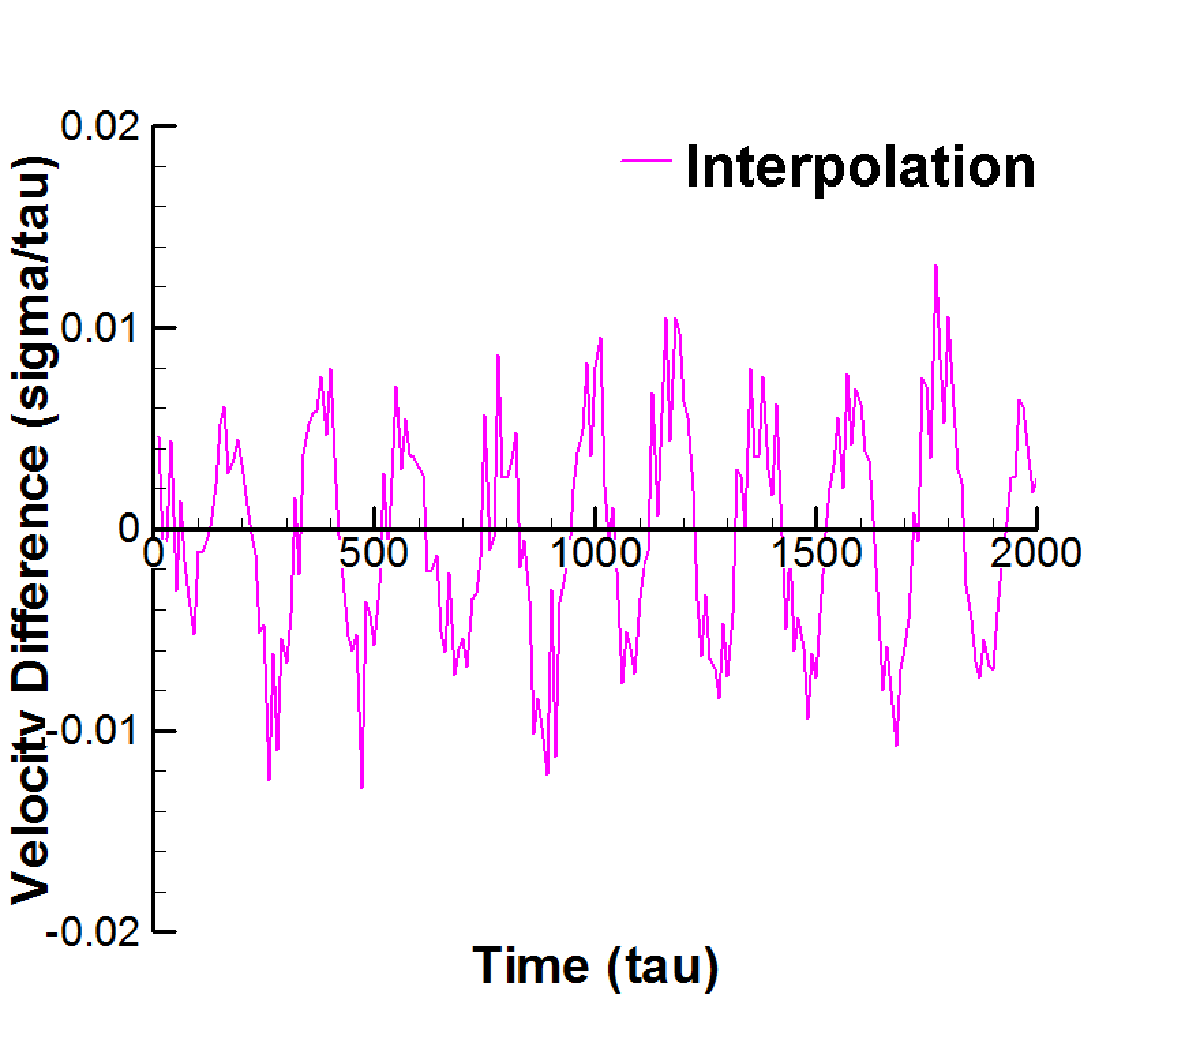
\includegraphics[width=0.45\linewidth]{Stokes_Imp_Diff.pdf}
\hskip 1cm
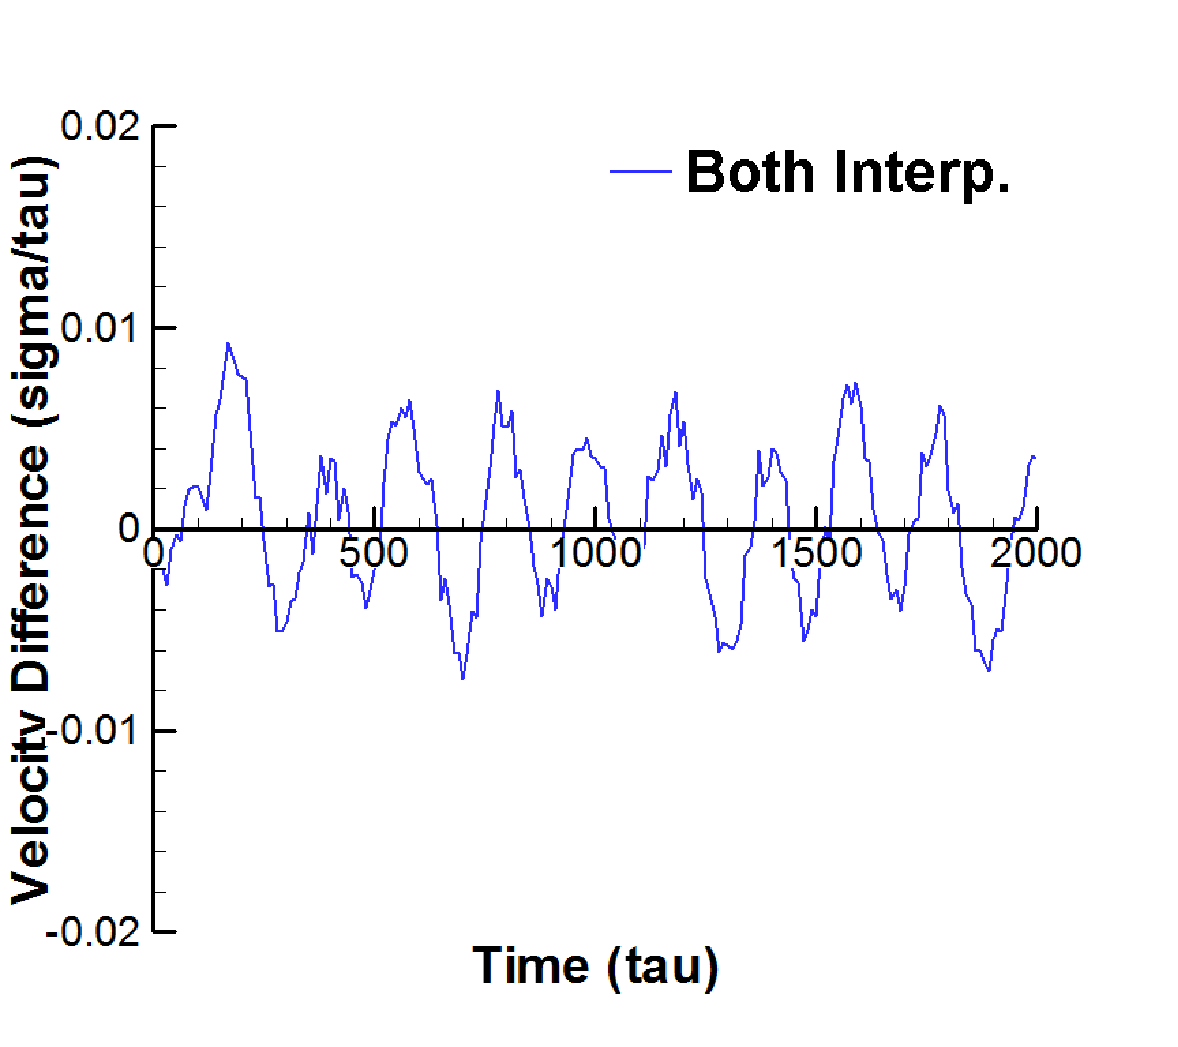
\includegraphics[width=0.45\linewidth]{Stokes_Both_Diff.pdf}
\caption{\small Reduction of Unsteady Error by Prediction-Correction Approach; Figures show the velocity difference between pure CFD and hybrid solutions in the middle of hybrid layer. Plotted data include the conventional extrapolation model and 3 different types of prediction-correction approaches, which are corrected extrapolation model, interpolated boundary model on MD domain and interpolated boundary condition on both domains. The velocity difference in the conventional model ranges from -0.017 to 0.015. This error reduces to be within -0.007 and 0.009 in refined model.}
\label{Temporal2}
\end{figure}


\section{Performance Analysis of a Multi-physics Simulation Framework}
\label{sec:performance}

The benefit of a BigJob as a way of reducing the waiting time on the local queueing system can be discussed from our preliminary test of the relationship between the requested number of processors and the waiting time.

%We designed experiments to determine if running larger and/or longer simulations effects the actual waiting time on the queue. We performed our experiments on machines spanning two orders of magnitude in size (and peak performance)-- from approximately 500 px to 65000 px, and for a range of load-factors.  We submitted jobs of different sizes, requiring different wall-time limits. Each time we submitted a job, we gathered the load-factor and the actual waiting time on the queue. Many factors effect the waiting times, arguably the most important of them are the load-factor at the instant of submission, requested wall-time limit and also the number of processors requested. Two other factors that effect this are the backfilling that occurs when some other unrelated job finishes and the changes in the priority of the test job when a particular higher priority job joins the queue; however, unlike the first three factors, the last two are somewhat random and it is difficult to systematically account for them. Also, the internal queueing policy of supercomputing centers may effect the waiting time on the queue based on their queueing priority including credential, fairshare, resource and service priority.  As can be seen from Table~\ref{table:waitingtime}, the waiting time tends to decrease as the number of processors requested in a job increases.

%Results for machines with more than 5000 px, Ranger and Queenbee are presented in Table~\ref{table:waitingtime}, and as can be seen, jobs with larger processor counts have typically lower wait times. The observation holds true for a range of values of requested wall-times over a range of ``high'' load-factors.


%\begin{table}
%  \caption{\small  Effect of various configurations on waiting time. The tables show the queue waiting times on Ranger and QueenBee with a changing number of processors and different requested resource wall-time limits. Analyzing the actual waiting time as a function of the number of processors at different wall-time limits, it can be said that better more often than not, the waiting time decrease as the requested number of processors increases. The relationship between the waiting time and wall-time limit is harder to quantify. However, obtained numbers provide a good case study for showing the variance of actual queue waiting times.}
%\label{table:waitingtime}
%\centering
%\footnotesize
% \begin{tabular} {c || p{0.1\linewidth} p{0.1\linewidth} p{0.1\linewidth} p{0.1\linewidth} p{0.1\linewidth} }
% \multicolumn{6}{c}{\phantom{\tiny 100}}\\
%\hline
% \multirow{3}{0.15\linewidth}{Number of processors}&
% \multicolumn{5}{c}{Requested wall-time at 92$\pm$6\% load (Ranger)} \\
%\cline{2-6}
% & \nyc 2hr & \nyc 3hr & \nyc 4hr & \nyc 6hr & \multicolumn{1}{c}{12hr} \\
%\cline{2-6}
% &\multicolumn{5}{c}{Waiting time on the queue [sec]} \\
%\cline{1-1}
%\nyc 16 & \nyc 9989 & \nyc 15984 & \nyc 39151 & \nyc 65 & \multicolumn{1}{c}{66} \\
%\nyc 32 & \nyc 15371 & \nyc	4106 & \nyc 11376 & \nyc 54 & \multicolumn{1}{c}{55} \\
%\nyc 48 & \nyc 13264 & 4392 \nyc  & \nyc 37780 &\nyc 43 & \multicolumn{1}{c}{44} \\
%\nyc 64 & \nyc 9944 &	\nyc 1975	 & \nyc 39855 & \nyc 31 & \multicolumn{1}{c}{32} \\
%\hline

%\multicolumn{6}{c}{\phantom{100}}\\
%\hline
% \multirow{3}{0.15\linewidth}{Number of processors}&
% \multicolumn{5}{c}{Requested wall-time at 95$\pm$4\% load (Queenbee)}\\
%\cline{2-6}
% &\nyc 2hr &\nyc 3hr &\nyc 4hr &\nyc 6hr &\multicolumn{1}{c}{12hr}\\
%\cline{2-6}
% &\multicolumn{5}{c}{Waiting time on the queue [sec]}\\
%\cline{1-1}
%\nyc 16 & \nyc 14339 & \nyc 3578  & \nyc 39113 & \nyc 6 & \multicolumn{1}{c}{940}\\
%\nyc 32 & \nyc 14312 & \nyc 3550 & \nyc 39238 & \nyc 5 &\multicolumn{1}{c}{6344}\\
%\nyc 48 & \nyc 21555 & \nyc 3517 & \nyc 39207 & \nyc 4 & \multicolumn{1}{c}{6353}\\
%\nyc 64 & \nyc 21541 & \nyc 3489 & \nyc 39179 & \nyc 3 & \multicolumn{1}{c}{6329}\\
%\hline
%\end{tabular} %}
%\vspace{-1em}
%\end{table}


%It is however, difficult to discern a relationship between waiting time with the requested wall-time limit of jobs; from experience there is greater variation in backfilling probability with varying wall-time requests.  However, as we are able to establish that a single large job on average has to wait less at the queue than a smaller job does, most definitely the maximum wait time of two small jobs will be even greater. In other words the sum total of the waiting time (of the first-to-run job) and the inactive time (defined as the difference between the waiting time of the two jobs) will be larger than the wait time of a single large job.



We designed experiments to determine if running larger and/or longer simulations effects the actual waiting time on the queue. We performed our experiments on a sufficiently large system in size -- around 65000 px. We submitted jobs of different sizes, requiring different wall-time limits. Each time we submitted a job, we gathered the actual waiting time on the queue. Many factors effect the waiting times, arguably the most important of them are the existing job requests on the resource at the instant of submission, requested wall-time limit and also the number of processors requested. Two other factors that effect this are the backfilling that occurs when some other unrelated job finishes and the changes in the priority of the test job when a particular higher priority job joins the queue. Of these factors, number of requested resources and wall time limits are what can be handled by users and can be systematically accounted for. Also, the internal queueing policy of supercomputing centers may effect the waiting time on the queue based on their queueing priority including credential, fairshare, resource and service priority. As can be seen from Table~\ref{table:WaitTime}, jobs with larger processor counts have typically lower wait times. The observation holds true for a range of values of requested wall-times.

\begin{table}
  \caption{\small Effect of Various Configurations on Waiting Time; The tables show the queue waiting times on Ranger depending on the number of processors and requested wall-time limits. Analyzing the actual waiting time as a function of the number of processors at different wall-time limits, it can be said that better more often than not, the waiting time decrease as the requested number of processors increases. The relationship between the waiting time and wall-time limit is harder to quantify. However, obtained numbers provide a good case study for showing the variance of actual queue waiting times. 10 independent experiments are sampled and expressed in seconds as "mean$\pm$SD".}
  \label{table:WaitTime}
  \centering
%  \resizebox{0.8\linewidth}{!} {
\footnotesize
  \begin{tabular}{c || c c c}
 \multicolumn{4}{c}{\phantom{\tiny 100}}\\
\hline
 \multirow{2}{0.15\linewidth}{Number of Processors} &
 \multicolumn{3}{c}{Requested Walltime on Ranger} \\
\cline{2-4}
& 6 Hrs & 24 Hrs & 48 Hrs\\
\hline			
128  &  24287.14\scriptsize{$\pm$15724.91}  &  25941.71\scriptsize{$\pm$13878.78}  &  44012.14\scriptsize{$\pm$44537.75} \\
256  &  27606.57\scriptsize{$\pm$19207.95}  &  26878.86\scriptsize{$\pm$15108.29}  &  67876.29\scriptsize{$\pm$70713.95} \\
512  &  27930.43\scriptsize{$\pm$18496.98}  &  24361.43\scriptsize{$\pm$14849.23}  &  32097.14\scriptsize{$\pm$27617.86} \\
1024  &  13514.57\scriptsize{$\pm$11373.68}  &  16372.43\scriptsize{$\pm$10857.48}  &  22134.71\scriptsize{$\pm$11089.26} \\

\hline
\end{tabular} %}
\vspace{-1em}
\end{table}

It is however, difficult to discern a relationship between waiting time with the requested wall-time limit of jobs; from experience there is greater variation in backfilling probability with varying wall-time requests. However, as we are able to establish that a single large job on average has to wait less at the queue than a smaller job does, most definitely the maximum wait time of two small jobs will be even greater. In other words the sum total of the waiting time (of the first-to-run job) and the inactive time (defined as the difference between the waiting time of the two jobs) will be larger than the wait time of a single large job.



\skonote{Queue Wait Time Analysis: Waiting time of a BigJob and two conventional jobs. Emphasize the inactive time as well - it makes the conventional job submission to have longer wall time limit and it will even reduce the possibility of getting the backfilling capability. Include Table 2 here.}

A BigJob submission shows the saving of waiting time on the queue, not only the bigger job size has the higher priority in the queueing system but also one BigJob submission eliminates the inactive idling time of first allocated job in conventional job submission.

\skonote{More test conducted on Ranger. Table needs replacement.}

\begin{table}
  \caption{\small Waiting and inactive time for conventional job submissions, and a single BigJob submission. All measured times are in seconds. In the first two cases, conventional job is submitted to use 2$\times$128 px and a BigJob requests 256 px: latter two cases use 2$\times$256 and 512 px, respectively. Conventional job submission mode showed faster time-to-start (i.e., waiting time of the first job + inactive mode) on small problem size with 6 hr of wall-time limit, while a BigJob gets allocated faster with longer wall-time limit. Conventional job submission showed 3 failures during the test due to the timeover of wall-time limit in the first-started job.}
\label{table:BJwaiting}
\centering
\footnotesize
 \begin{tabular}{c | c | c | c }
 \multicolumn{4}{c}{\phantom{\tiny 100}}\\
\hline
px & Wall-time & Scenario & Time-to-start\\
\hline
\hline
\multirow{4}{0.1\linewidth}{256} & \multirow{2}{0.1\linewidth}{6 Hrs} & S0 & 15770.8 + 1085.9\\
\cline{3-4}
&  & S1 & 15200.2\\
\cline{2-4}
& \multirow{2}{0.1\linewidth}{24 Hrs} & S0 & 4797.7 + 10363.5\\
\cline{3-4}
&  & S1 & 11455.3\\
\hline
 \multirow{4}{0.1\linewidth}{512}& \multirow{2}{0.1\linewidth}{6 Hrs} & S0 & 15514.0 + 449.4\\
\cline{3-4}
&  & S1 & 15825.4\\
\cline{2-4}
& \multirow{2}{0.1\linewidth}{24 Hrs} & S0 & 4181.5 + 11098.5\\
\cline{3-4}
&  & S1 & 13627.9\\
\hline
\end{tabular} %}
%\begin{tabular}{c | c | c | c c}
% \multicolumn{5}{c}{\phantom{\tiny 100}}\\
%\hline
%px & wall-time & scenario & queue waiting & inactive mode\\
%\hline
%\hline
%\multirow{4}{0.1\linewidth}{256} & \multirow{2}{0.1\linewidth}{6 Hrs} & S0 & 15770.8 & 1085.9\\
%\cline{3-5}
%&  & S1 & \multicolumn {2}{c}{15200.2}\\
%\cline{2-5}
%& \multirow{2}{0.1\linewidth}{24 Hrs} & S0 & 4797.7 & 10363.5\\
%\cline{3-5}
%&  & S1 & \multicolumn {2}{c}{11455.3}\\
%\hline
% \multirow{4}{0.1\linewidth}{512}& \multirow{2}{0.1\linewidth}{6 Hrs} & S0 & 15514.0 & 449.4\\
%\cline{3-5}
%&  & S1 & \multicolumn {2}{c}{15825.4}\\
%\cline{2-5}
%& \multirow{2}{0.1\linewidth}{24 Hrs} & S0 & 4181.5 & 11098.5\\
%\cline{3-5}
%&  & S1 & \multicolumn {2}{c}{13627.9}\\
%\hline
%\end{tabular} %}
\vspace{-1em}
\end{table}

Controlling runtime in these two scenarios, i.e., we take a BigJob of size 2X and 2 conventional jobs of size X each, we compare the waiting time of a 64 px BigJob (with wall-clock limits of 2, 3, and 4hrs) which is smaller than the wait for a 32 px conventional job for the same values of wall-clock limits. As the individual simulations are assigned the same number of processors, the runtime performance will be similar in the two scenarios, and thus the total time-to-solution will determined by the wait-times on queues -- which we show statistically to be lower for the larger BigJob submission mode.

%\begin{table}
%  \caption{\small  Waiting and inactive time for conventional job submissions, and a single BigJob submission. All measured times are in seconds and expressed as 'mean$\pm$SD'. In both cases, conventional job is submitted to use 2$\times$32 px and a BigJob requests 64 px on small and less crowded LONI clusters. Conventional job submission mode showed faster time-to-start (i.e., the sum of waiting time and inactive mode) on small problem size with 6 hr of wall-time limit, while a BigJob gets allocated faster with longer wall-time limit. Conventional job submission showed 3 failures during the test due to the timeover of wall-time limit in the first-started job.}
%\label{table:BJwaiting}
%\centering
%\footnotesize
% \begin{tabular}
% {>{\centering}p{0.15\linewidth} || p{0.2\linewidth} p{0.2\linewidth} p{0.2\linewidth} }
%\multicolumn{4}{c}{\phantom{\tiny 100}}\\
%\hline
% \multirow{2}{0.55in}{}& \multicolumn{3}{c}{Small simulation with 6 hr wall-time limit}\\
%\cline{2-4}
% & \nyc Waiting time & \nyc Inactive mode & \multicolumn {1}{c}{Failed runs}\\
% \hline
%   \nyc Conventional & \nyc 12318$\pm$15649 & \nyc 7407$\pm$11375 & \multicolumn {1}{c}{2} \\
%  \nyc 1 BigJob & \nyc 29452$\pm$31946 & \nyc 0 & \multicolumn {1}{c}{0} \\
% \hline
%\multicolumn{4}{c}{\phantom{100}}\\
%\hline
% \multirow{2}{0.55in}{}& \multicolumn{3}{c}{Large simulation with 24 hr wall-time limit}\\
%\cline{2-4}
% & \nyc Waiting time & \nyc Inactive mode & \multicolumn {1}{c}{Failed runs}\\
%\hline
% \nyc Conventional & \nyc 83102$\pm$77134 & \nyc 47488$\pm$55647 & \multicolumn{1}{c}{1}\\
% \nyc 1 BigJob & \nyc 76645$\pm$55474 & \nyc 0 & \multicolumn{1}{c}{0}\\
%\hline
%\end{tabular} %}
%\vspace{-1em}
%\end{table}


Results for smaller systems ($\approx$ 500 px) are presented in a different fashion in Table~\ref{table:BJwaiting}. In addition to the fact that a 64 px BigJob is now around 16\% of the machine resources, the load-factors of the smaller machines fluctuated much more than those of the larger machines. Consequently the data obtained for smaller resources is far more noisier and than the ``clean'' data for the larger machines -- Ranger and QueenBee. As can be seen from Table~\ref{table:BJwaiting} although the waiting time for the first-to-start job was smaller in the conventional job submission mode than the BigJob (S1), the second job (convention job) had a large subsequent wait time; thus for conventional job submission mode there is a non-negligible inactive mode (defined as the time difference between queue wait times between the two simulations). There is no inactive mode for BigJob submission as by defintion both simulations begin concurrently. Interestingly, the situation is somewhat worse for the conventional job submission; although the average wait time is lower than the BigJob, there exist 2 (out of 6) cases (for 6hr wall-clock limit), when the wait time of the second job is greater than the wall-clock limit for the first-to-start job. In other words, the second job fails to start in the duration that the first-to-start job is in active/run mode, but can't do anything useful as the second job is still waiting on the queue. This is typically alleviated with co-allocation of resources; however the number of production grid infrastucture that provide co-allocation (and co-scheduling) as a production service is very limited. This leads us to the heart of the advantage of the BigJob submission mode: circumventing the requirements of co-scheduling by providing an application level solution that preserves performance and guarantees non-failure due to large-fluctuations (see data for 24hr wall-time limit) in queue waiting times.



\skonote{Runtime Analysis: Comparison of LB with conventional simulation time: different system size (with different ratio between CFD and MD), different number of simulation loop and different interval of simulation loop. Table 3 with 2 graphs - change of CPU allocation to each subjob with iteration time in 2 simulation cases. Mention the problem size and setting a little more detail.}

Runtimes of the coupled simulation with a single BigJob is given on Table~\ref{table:oneBJ_Test}. For both small and large simulations, a default BigJob task takes about 1 percent longer than the conventional test. This is reasonable because a default BigJob has the same processor distribution between sub-jobs as the conventional job, while BigJob has the minor overhead of sub-jobs' status monitoring and communication with advert server. In cases of load-balanced BigJob simulations, there is a significant reduction in the runtime compared to successful conventional jobs -- 13\% and greater. For larger problem set, a load-balanced BigJob simulation relatively shows higher standard deviation (SD) due to the unexpected instability of a computing resource during one experiment, to be discussed in detail below.

\begin{table}
  \caption{\small Results of runtime for S1, $S1_{LB}$ and conventional submission. All measured times are in seconds and expressed as 'mean$\pm$SD'. 6 distinct experiments were accomplished for each simulation, all with 64 px. In both cases, S1 shows about 1\% overhead due to the communication with advert server. On the other hand, $S1_{LB}$ tests show about 13\% runtime save compared to conventional submission.}
\label{table:oneBJ_Test}
\centering
\footnotesize
\begin{tabular} {>{\centering}p{0.15\linewidth} || p{0.15\linewidth} p{0.15\linewidth} p{0.15\linewidth} }
  \multicolumn{4}{c}{\phantom{\tiny 100}}\\
  \hline
  & \nyc Conventional  & \nyc S1  & \multicolumn{1}{c}{$S1_{LB}$}  \\
  \hline
  \nyc Small sim. & \nyc 757$\pm$1.89 & \nyc 764$\pm$1.41 & \multicolumn{1}{c}{661$\pm$4.41} \\
  \nyc Large sim. & \nyc 39595$\pm$119.2 & \nyc 39906$\pm$206.3 & \multicolumn{1}{c}{34350$\pm$1302.7} \\
  \hline
\end{tabular} %}
\vspace{-1em}
\end{table}

The validity of a load-balancing function can be discussed by the change of processor distribution between subtasks throughout the simulation. For the result of a small simulation in Fig.~\ref{Fig:LBSmall}, both CFD and MD subtasks are assigned with 32 px initially. After two simulation loops, a load balancer converges to the processor distribution of 12 to 52 px between CFD and MD respectively; this processor distribution remains the same until the simulation completes. Runtime per loop is reduced from 153 sec for the first loop to 107 sec after the convergence. Total computation time is 596.19 sec, which is different from 663 sec counted from BigJob application manager. This time difference implies that the BigJob application manager spends about 13 sec per stage in executing its internal commands including the run of a load-balancing function and sub-job re-launch.


%%%%% FIGURE %%%%%
\begin{figure}
%\vspace{-1em}
\centering
%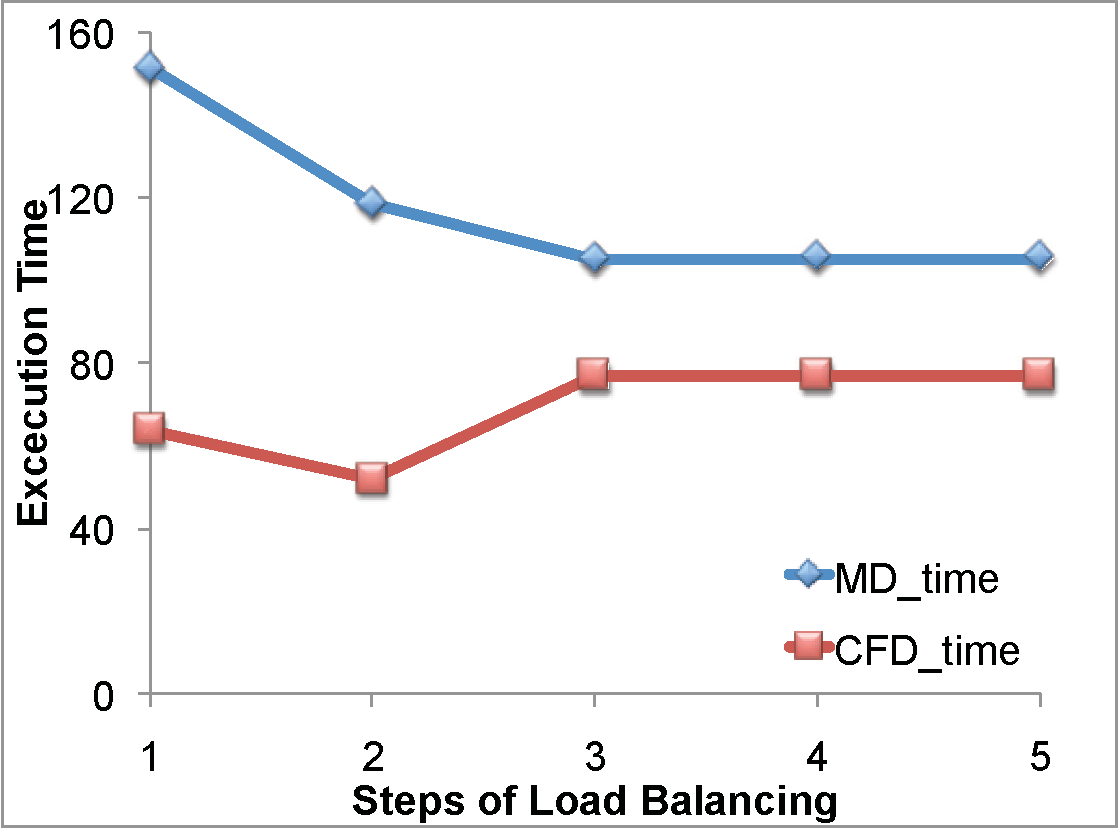
\includegraphics[scale=0.3]{fig6_1.pdf}
\includegraphics[width=0.4\linewidth]{BJ_Small_Cost.eps}
%\linebreak
%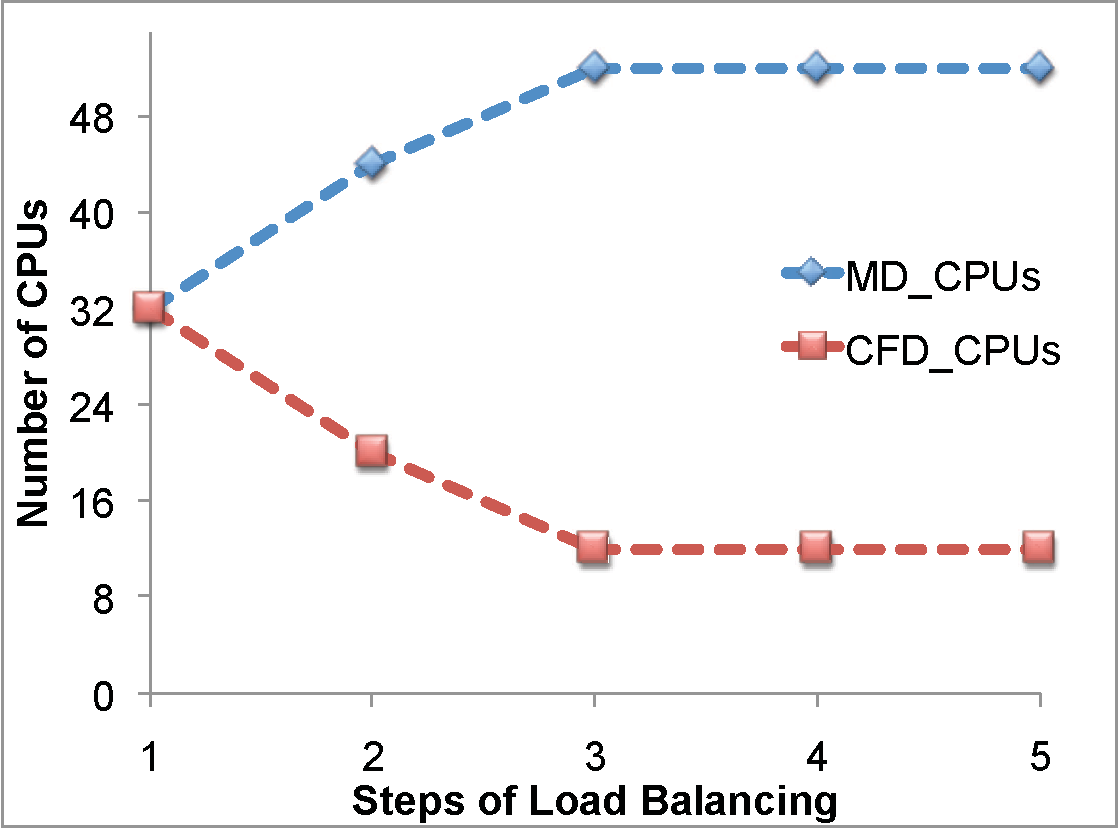
\includegraphics[scale=0.3]{fig6_2.pdf}
\includegraphics[width=0.4\linewidth]{BJ_Small_Proc.eps}
\caption{\small Change of processor distribution between CFD and MD
  jobs and resultant computation time in the small simulation. A load
  balancer starts from the same number of processors assigned to both
  sub-jobs and detects 20 to 44 px between each sub-job as the optimal
  solution. The poor scalability of CFD job makes the load balancer to
  search for the optimal condition once again and the processor
  assignment finally reaches to a steady solution of 12 to 52 between
  two sub-jobs. Computation time for every simulation loop reduces
  from 153 sec to 107 sec after the balancing.}
\label{Fig:LBSmall}
\vspace{-1em}
\end{figure}
%%%%% FIGURE %%%%%


The result of computation time evolution for a large simulation is seen in Fig.~\ref{Fig:LBLarge}. For most experiments, which is given in the left side of Fig.~\ref{Fig:LBLarge}, a load balancer directly goes to a converged solution of processor distribution, which is 24 to 40 between CFD and MD jobs. On the other, in one experiment, computing nodes assigned to MD simulation seem to have temporarily experienced the internal overhead as shown from the right side of Fig.~\ref{Fig:LBLarge}. This overhead temporarily increased MD computation time a lot and a load balancer shows the fluctuating pattern of processor distribution in response to this temporary instability. A load balancer goes to a different steady solution after the system settled down, which is the processor distribution of 20 to 44 between two sub-jobs. Compared to the steady solution in stable cases, computation time for one simulation loop increases in this processor distribution increases from 1320 sec to 1380 sec.

Plots on the right side of Fig.~\ref{Fig:LBLarge} show a non-monotonically changing resource assignment by the LB, and thus demonstrating how the load balancer can be self-correcting and adapt to changing performance; after increasing the number of processors assigned to the MD, the load-balancer unassigns the additional processors.


% %%%%% FIGURE %%%%%
\begin{figure}
%\vspace{-1em}
\centering
%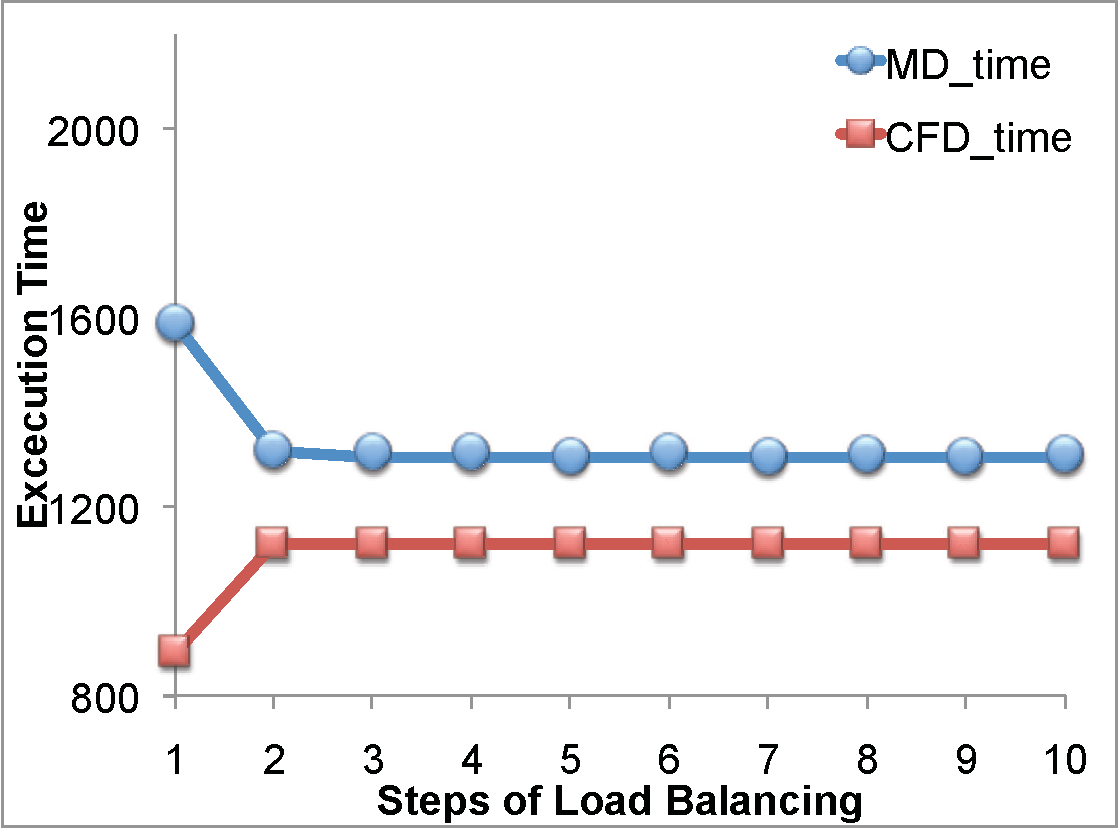
\includegraphics[scale=0.21]{fig7_11.pdf}
\includegraphics[width=0.4\linewidth]{BJ_Large_Cost_Normal.eps}
%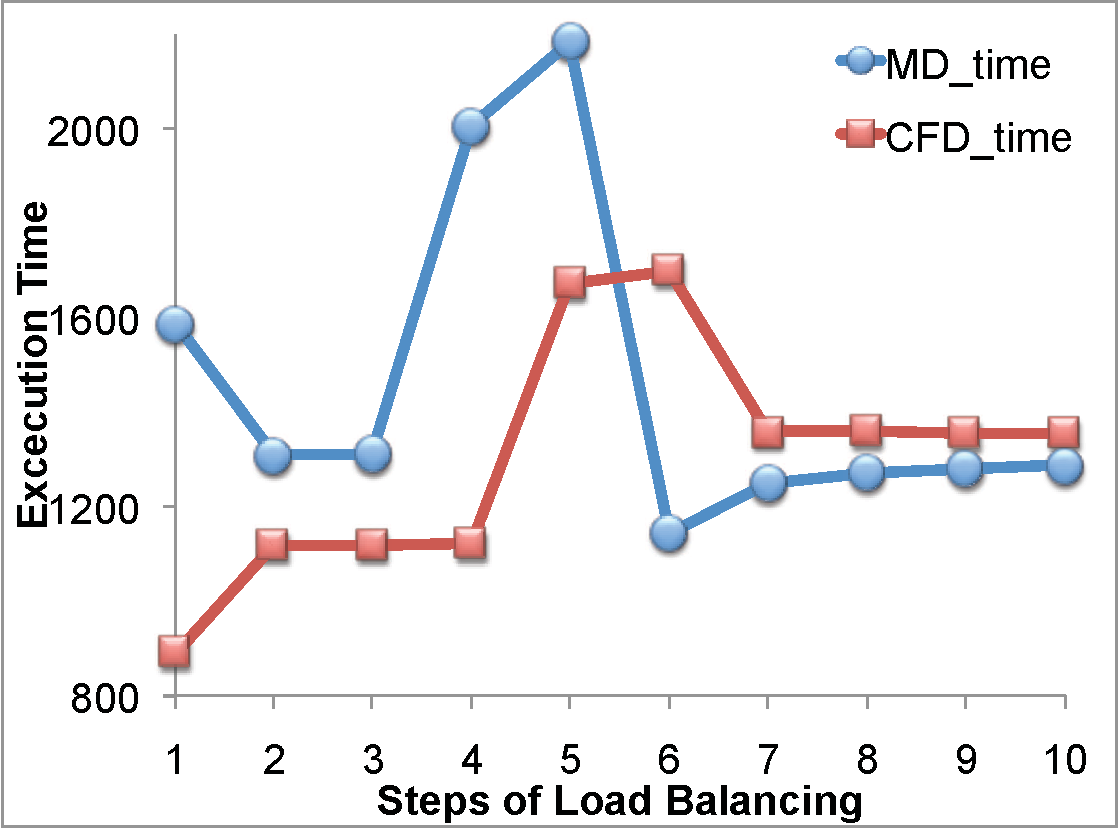
\includegraphics[scale=0.21]{fig7_21.pdf}
\includegraphics[width=0.4\linewidth]{BJ_Large_Cost_Abnormal.eps}
\linebreak
%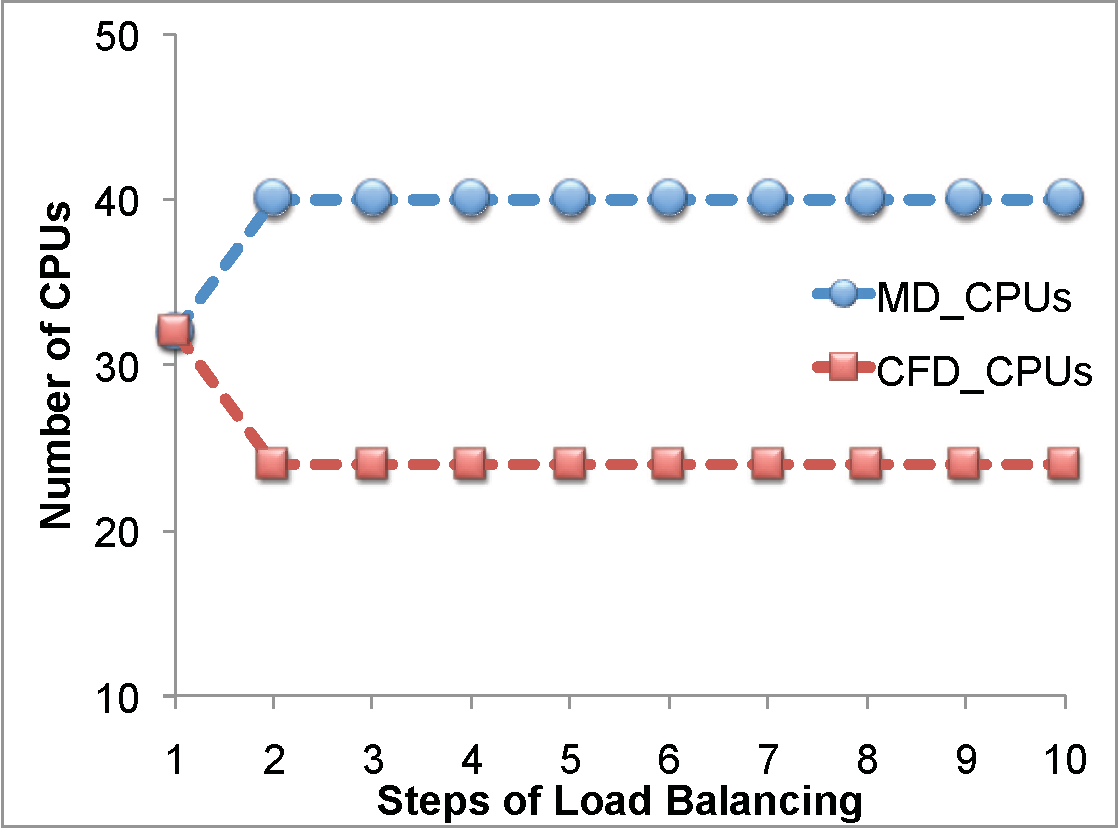
\includegraphics[scale=0.21]{fig7_12.pdf}
\includegraphics[width=0.4\linewidth]{BJ_Large_Proc_Normal.eps}
%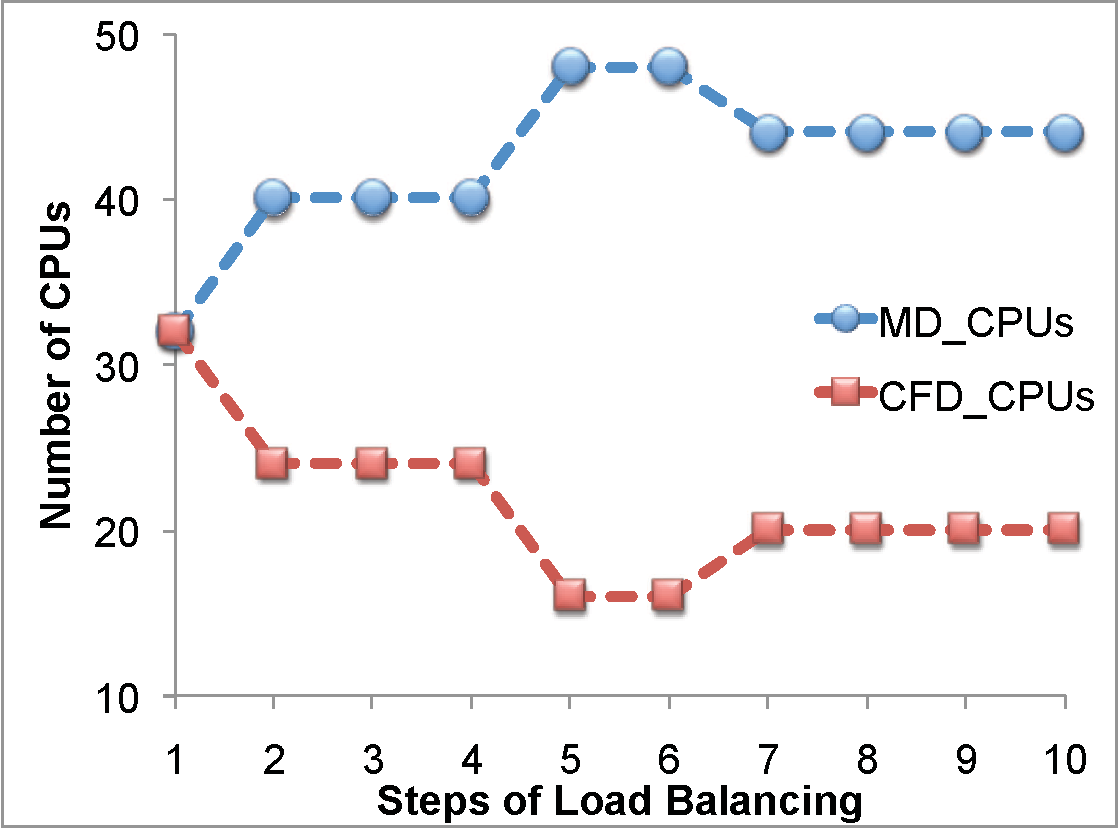
\includegraphics[scale=0.21]{fig7_22.pdf}
\includegraphics[width=0.4\linewidth]{BJ_Large_Proc_Abnormal.eps}
\caption{\small (Left Column) Change of processor distribution between
  CFD and MD jobs and resultant computation time in the large
  simulation. A load balancer directly finds the processor
  distribution of 24 to 40 between CFD and MD jobs and remains the
  steady state until it completes after 25 simulation loops. Initial
  computation time of 1605 sec reduces to 1320 sec after the
  convergence. (Right Column) Plots showing non-monotonic resource
  assignment by the LB, and thus demonstrating how the load balancer
  can be self-correcting and adapt to changing performance; after
  increasing the number of processors assigned to the MD, the
  load-balancer unassigns the additional processors.}
\label{Fig:LBLarge}
\vspace{-1em}
\end{figure}
%%%%% FIGURE %%%%%



%-------------------------------------------------------------------------
\section{Next Step: Further Refinement}
\label{sec:futureworks}

The empirical mathematical equation on sampling noise has been presented in Sec.~\ref{sec:accuracy_conditions}. We argue that this is a refined model compared to previous mathematical expressions. However, the formulation has not been verified by various systems and conditions: coefficients will be changing according to the distance from the wall, characteristics of fluid and solid elements, etc. More rigorous research is required to address a globally acceptable equation of sampling noise.

Unsteady flow simulation in Sec.~\ref{sec:accuracy_oscillation} verifies that the prediction-correction approach provides more accurate solution than conventional temporal coupling scheme. The new approach is especially powerful in resolving the unfavorable overshoot/undershoot phenomena. On the other hand, the slight time-lagging effect in the conventional model has not been improved by the prediction-correction approach. We expect that this phenomenon can be resolved by applying higher-order extrapolation/interpolation on hybrid boundary regions.

%The unstable solution at Fig.~\ref{Couette_Noisy} represents the result of Couette flow simulation with 0.1 $\sigma / \tau$ upper plate velocity in O(100) nanometer system. The diverging solution is intuitively natural, according to the statistical noise measurement in Table~\ref{table:MD_Vel0_L}: the amount of statistical error is 25 percent of the steady-state velocity in MDtoCFD layer. For the worse, the signal-to-noise ratio is even larger at early stage. Thus the strong initial instability makes it harder for the solver to reach the steady-state solution. Increasing the sampling duration to 1000 $\tau$ did not help; increasing the height of layers implies the abandonment of hybrid method's merit over pure MD method.
%Clearly, this is one of the most important issues to make the family of hybrid methods a powerful tool which describes the detailed phenomena between solid obstacles and surrounding fluids more accurately. So far, two possible ways are observed at the first glance. First, setting the initial MD condition the same as steady-state CFD profile and starting hybrid simulation will, at least, alleviate the influence of noise at early stage. However, time-accurate unsteady solution can not be gained by this approach. Second, \skonote{check the clear term of zeta at Nie's formulation!} increasing $\zeta$ looks helpful in alleviating the noise in system level. However, this is worried whether excessive suppress of particles' vibration results in the breakup of fluid physics, i.e., breakup of energy conservation. A thorough investigation on the characteristics of statistical noise and design of numerical algorithm for acquiring the accurate solution without numerical damping are highly required.

%%\begin{figure}[ht!]
%\begin{figure}
%\centering
%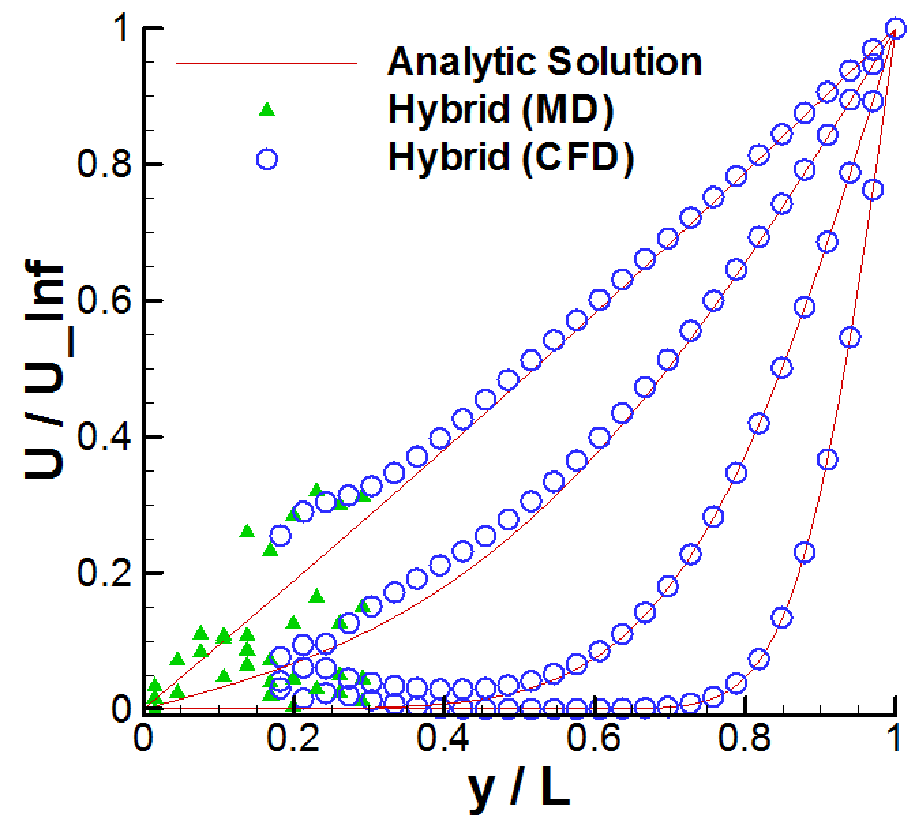
\includegraphics[width=0.6\linewidth]{Couette_Noisy.pdf}
%\vskip-0.2cm
%\caption{\small Unstable Solution at Low Shear Rate; Velocity of the upper plate is 0.1 $\sigma / \tau$ and all other conditions are identical to the Couette flow simulation in large domain. The solution diverges at early stage, since the statistical error is very large compared to the hydrodynamic velocity.}
%\label{Stokes_Sol}
%\end{figure}



%-------------------------------------------------------------------------
\section{Conclusions}
\label{sec:conclusion}

Accurate and efficient multi-scale flow simulations by a hybrid CFD-MD simulation framework have been presented in this paper. Constrained Lagrangian dynamics equations of motion and file-based hybrid interfaces are implemented on a highly-reliable LAMMPS molecular dynamics package and a verified in-house incompressible CFD code. They are virtually integrated as a single BigJob framework.

A number of numerical issues which harm the accuracy of a hybrid solution have been explored. First, quantifying the sampling noise from a stationary flow has been proposed as a way of determining coupling parameters. We argue that our simple and intuitive idea unveils the influence of individual coupling parameter on the magnitude of statistical error and is very cost-effective in contrast to traditional trial-and-error approach.
%until getting a stable solution.
Moreover, the empirical equation derived from the stationary flow simulation describes that well-know mathematical expressions on statistical error are not accurate on nano-scale wall-bounded systems.
Second, sampling multiple independent replicas has been introduced to refine the sampling noise of an individual solution and to explore to the low-speed flow regimes. This approach is superior to simulating a single large-scale problem set which is technically bound by computing capacity. The application to a Couette flow simulation in O(10) m/s velocity field is the first successful report of a moderate-speed flow simulation using a hybrid CFD-MD approach.
Last, a prediction-correction approach has been designed for the accurate unsteady simulation. This approach acquires better solution by enabling the imposition of interpolated hybrid boundary conditions. The application to the oscillating boundary problem expresses that the current approach diminishes the overshoot/undershoot phenomena in the conventional methods.

Along with numerical issues, computational issues for the efficient coupled simulations have been also discussed. We introduced a BigJob framework and this directly solves the co-scheduling problem among logically separated sub-tasks. A simple load balancing function is also implemented on a BigJob framework, to achieve the load balancing among those separated-yet-coupled codes. From numerical experiments, we evaluate that a BigJob is very powerful in reducing the waiting time of the coupled simulation. Also, a simple load balancing function employed in a BigJob is effective in reducing the simulation runtime.

We emphasize that above numerical investigations ease the challenge to the hybrid simulation and broaden the application area. Also, our computational experiments contribute on how to efficiently conduct coupled simulations.
\skonote{Plz fill this last paragraph!}

\section*{Acknowledgements}
This work is part of the Cybertools (http://cybertools .loni.org)
project and primarily funded by NSF/LEQSF (2007-10)-CyberRII-01.
Important funding for SAGA has been provided by the UK EPSRC grant
number GR/D0766171/1 (via OMII-UK) and HPCOPS NSF-OCI 0710874. This
work has also been made possible thanks to computer resources provided
by TeraGrid TRAC TG-MCB090174 and LONI resources.

%% The Appendices part is started with the command \appendix;
%% appendix sections are then done as normal sections
%% \appendix

%% \section{}
%% \label{}

%% References
%%
%% Following citation commands can be used in the body text:
%% Usage of \cite is as follows:
%%   \cite{key}         ==>>  [#]
%%   \cite[chap. 2]{key} ==>> [#, chap. 2]
%%

%% References with bibTeX database:

\bibliographystyle{elsarticle-num}
\bibliography{saga_tg08}

%% Authors are advised to submit their bibtex database files. They are
%% requested to list a bibtex style file in the manuscript if they do
%% not want to use elsarticle-num.bst.

%% References without bibTeX database:

% \begin{thebibliography}{00}

%% \bibitem must have the following form:
%%   \bibitem{key}...
%%

% \bibitem{}

% \end{thebibliography}


\end{document}

%%
%% End of file `elsarticle-template-num.tex'.
